%
%  --- USU thesis and dissertation template ---
%
% Time-stamp: "[thesis.tex] last modified by Scott Budge (scott) on 2019-05-08 (Wednesday, 8 May 2019) at 19:28:11 on goga.ece.usu.edu"
%
%  Modified to use the new usuthesis.cls by Allan McInnes
%
%  Specify department ('ee' or 'ce' or 'me' or 'ae' or 'cee') and document type ('msthesis',
%  'msreport', or 'dissertation') in the documentclass options. 
%
%  Including the 'proposal' option will generate a proposal for a thesis
%  or dissertation, rather than a final document (this mostly just 
%  alters the cover page).
%
%  See the opening comments of usuthesis.cls for more information on 
%  available options
%
%  To create finished document run:
%    latex thesis.tex
%    bibtex thesis (or sample-chapter1, etc., if using multiple-paper format)
%    latex thesis.tex
%    latex thesis.tex
%
%  Info: $Id: thesis.tex 1142 2019-05-09 01:41:53Z scott $   USU
%  Revision: $Rev: 1142 $
% $LastChangedDate: 2019-05-08 19:41:53 -0600 (Wed, 08 May 2019) $
% $LastChangedBy: scott $
%

% For the ECE Department:
%\documentclass[ee,msthesis]{usuthesis}
%\documentclass[ce,msthesis]{usuthesis}
%\documentclass[ee,dissertation]{usuthesis}
%\documentclass[ce,dissertation]{usuthesis}


% For the MAE Department:
\documentclass[me,msthesis]{usuthesis}  % Unfortunately, this template was made before we became MAE. So sorry.
%\documentclass[ae,msthesis]{usuthesis} %.        DON"T FORGET TO ALSO CHANGE LINE 90-110 appropriately          %%
%\documentclass[me,dissertation]{usuthesis} % Unfortunately, this template was made before we became MAE. So sorry.
%\documentclass[ae,dissertation]{usuthesis}
% For the CEE Department:
%\documentclass[cee,msthesis]{usuthesis}
%\documentclass[cee,dissertation]{usuthesis}


%{{{ Packages
\usepackage{amssymb}           % add ams symbols stuff
\usepackage{graphicx}          % add graphics
\usepackage{subcaption}
\usepackage{url}
\usepackage[nobottomtitles*]{titlesec}
\usepackage[all]{nowidow}
\usepackage{mathtools} 
\usepackage{epstopdf, epsfig}
%\usepackage{flafter}           % Cause floats to appear after
                               % environment.
%\usepackage{siunitx}           % Provides standard formatting of SI units.

% Include TikZ and PGF packages for high-quality graphics, schematics
% and plots. This is optional; at the current time, when run with
% latex to create a .dvi file, the xdvi viewer will produce incorrect
% formatting for the TikZ figures.  If the .dvi file is converted to
% pdf using "dvipdf" the resulting pdf file is correct.  If this
% example is used with  pdflatex, the resulting TikZ figures in the
% output look fine.
\usepackage{tikz}       		% The base tikz+pgf package
\usetikzlibrary{arrows,shapes}	% Optional tikz extensions
\usepackage[american]{circuitikz}	% TikZ-based package for schematic drawings
\usepackage{pgfplots}			% Tikz-based package for making plots 
\pgfplotsset{compat=1.6}        % This *might* be necessary for your
                                % version of pgfplots.
\graphicspath{{images/}}                                


\usepackage{hyperref} % Creates hyperlinks within document
\hypersetup{colorlinks=true, linkcolor=blue,
  citecolor=blue,urlcolor=blue} % Use when compiling the digital copy
% \hypersetup{colorlinks=true, linkcolor=black,
% citecolor=black,urlcolor=black} % Use when compiling the printed copy

% The following allows for hyperlinked DOIs to be inserted in the
% manuscript by using \doi{}.
\usepackage{doi}

% Set spacing around figures and tables to triple space
\setlength{\intextsep}{2em} % Vertical space above & below [h] floats
\setlength{\textfloatsep}{2em} % Vertical space below (above) [t] ([b]) floats

% The following is added if you are using the multiple-paper format to
% add references after each chapter:
%\usepackage[sectionbib]{chapterbib}

%}}}

% Creating Anton's own symbols
\newcommand\Rey{\mathit{Re}}
\newcommand\Pran{\mathit{Pr}}

% Author and Title Information
\author{Anton G. Kadomtsev}
\title{A Complicated and Impressive Sounding Title that is Too Long
  For a Single Line While Including Everything}

% The Committee
\majorprof{Som Dutta, Ph.D.}
\firstreader{Robert L. Forward, Ph.D.}
\secondreader{Albert Einstein, Ph.D.}
\thirdreader{Gottfried Liebniz, Ph.D.}
\fourthreader{Isaac Newton, Ph.D.}	

% Graduate Dean
\graddean{Richard Cutler, Ph.D.}
\deantitle{Vice Provost for Graduate Studies}

% Degree Information
%\degree{Master of Science}
\degree{Master of Science}
\month{August}
\gradyear{2023}

\begin{document}
    %{{{ Frontmatter
    \preliminaries   % set frontmatter style
    
    \maketitle
    \makecopyright        % optional
    
    %
%  Time-stamp: "[abstract.tex] last modified by Scott Budge (scott) on 2017-01-10 (Tuesday, 10 January 2017) at 16:54:14 on goga.ece.usu.edu"
%
%  Info: $Id: abstract.tex 998 2017-03-21 16:44:33Z scott $   USU
%  Revision: $Rev: 998 $
% $LastChangedDate: 2017-03-21 10:44:33 -0600 (Tue, 21 Mar 2017) $
% $LastChangedBy: scott $
%

\begin{abstract}
% A space is needed before the text starts so that the first paragraph
% is indented properly.

Direct Numerical Simulations (DNS) are performed on rotating 2D bodies in incompressible stratified flow. The effects of rotation, shape, and stratification on drag, lift, and flow structures such as internal gravity waves (IGW) are investigated. The Schwarz-spectral element method (Schwarz-SEM) is utilized through the use of a static background mesh and a rotating, conforming mesh to account for rotation and noncircular shapes; the meshes overlap for data exchange. The Boussinesq approximation is utilized to account for the effects of stratification in the Navier-Stokes equations. This Schwarz-SEM framework in stratification is validated against literature and established methods. We conduct cycle-averaging and phase-averaging of the drag and lift on the ellipses to isolate the different ways in which drag and lift are affected by the parameters of interest. We conduct a Hilbert transformation of the fields of the results to investigate directionality of the IGW by extracting the wave numbers in each direction. We run static and rotating circular cylinder simulation cases, along rotating ellipse cases of two different noncircular aspect ratios. We run simulations at different stratification levels, along with simulations in homogeneous flows. 

\end{abstract}


% Local Variables:
% TeX-master: "newhead"
% End:

    %
%  Time-stamp: "[publicabstract.tex] last modified by Scott Budge (scott) on 2011-08-09 (Tuesday, 9 August 2011) at 09:17:43 on goga"
%
%  Info: $Id$   USU
%  Revision: $Rev$
% $LastChangedDate$
% $LastChangedBy$
%

\begin{publicabstract}
% A space is needed before the text starts so that the first paragraph
% is indented properly.

The public abstract is to convey the purpose of the research to the
PUBLIC, so layman's terms should be used.


\end{publicabstract}


% Local Variables:
% TeX-master: "newhead"
% End:

    %
% This is an example of an dedication page.  This is optional,
% and can contain anything you want to say.
%
%  Time-stamp: "[dedication.tex] last modified by Scott Budge (scott) on 2011-08-08 (Monday, 8 August 2011) at 15:46:26 on goga"
%
%  Info: $Id$   USU
%  Revision: $Rev$
% $LastChangedDate$
% $LastChangedBy$
%

\begin{dedication}
\begin{center} 
To all the little people....
\end{center}
% 
% If you intend to have a dedication longer than one line, do not put
% it in a centering environment.  It will look better.
\end{dedication}
  % This is optional 
    %
% This is an example of an acknowledgements page.  This is optional,
% and can contain anything you want to say.
%
%
%  Time-stamp: "[acknowl.tex] last modified by Scott Budge (scott) on 2011-08-08 (Monday, 8 August 2011) at 15:45:15 on goga"
%
%  Info: $Id$   USU
%  Revision: $Rev$
% $LastChangedDate$
% $LastChangedBy$
%

\begin{acknowledgments} 
I am so happy that my advisor helped me. I would also like to thank my lab partner Aditya Parik for helping me learn and understand Linux and its tools. I would like to thank Holland Kartchner for his help in helping me learn Nek5000 tools. I also appreciate his help from when we took a graduate level fluid dynamics course as undergrads and when we took high-performance computing. I would like to thank Ketan Mittal for building the meshes that I used for the simulations, and also for the matlab script he provided for phase-averaging. 
\\
\begin{flushright} 
Anton G. Kadomtsev 
\end{flushright}
\end{acknowledgments}

     % This is optional
    
    \tableofcontents 
    \listoftables 
    \listoffigures
    
    %%
%  Time-stamp: "[notation.tex] last modified by Scott Budge (scott) on 2011-08-08 (Monday, 8 August 2011) at 15:48:03 on goga"
%
%
% This is an example of a notations page.  
% The publication guide does not specify a format.
% The example here is in tabular format.
%
% Please note that the symbols in this example are defined
% in a separate include file.
%  Info: $Id$   USU
%  Revision: $Rev$
% $LastChangedDate$
% $LastChangedBy$
%

\begin{notation}

\setlength{\tabcolsep}{3mm}
{\begin {tabular}{ll}
\multicolumn{2}{l}{\textbf{Events}}\\
$\Sigma$ & set of all events (universal alphabet)\\
$\tick$   & successful termination signal\\
$\tau$ & invisible (internal) event\\
$a.b.c$    & compound event\\
$c ? x$   &input on channel $c$\\
$c ! x$   &output on channel $c$\\
$\lchan c \rchan$   &set of all events associated with channel $c$\\
\multicolumn{2}{l}{\textbf{Traces}}\\
$\nil$ &empty sequence\\
$\lseq a_1, \ldots , a_n \rseq$ & sequence $a_1, \ldots , a_n$, in that order\\
$s_1 \cat s_2$ &$s_1$ concatenated with $s_2$, e.g. $\lseq a \rseq \cat \lseq b \rseq = \lseq a, b \rseq$\\
$s_1 \leq s_2$ &$s_1$ is a prefix of $s_2$, e.g.  $\lseq a \rseq \leq \lseq a, b \rseq$ \\
$s \hide X$ &hiding - all members of $X$ removed from $s$\\
$s \restrict X$ &restriction - hide all but members of $X$\\
$s \crestrict c$ &sequence of values in $s$ communicated over channel $c$\\
$s \seqcount a$ &number of $a$ events in $s$\\
\multicolumn{2}{l}{\textbf{Processes}}\\
$a \then P$ &prefixing\\
$P \interleave Q$ &interleaved parallel\\
$P \parallel[A][B] Q$ &alphabetized parallel\\
$P \parallel[X] Q$ &interface parallel\\
$P \extchoice Q$ &external choice\\
$P \intchoice Q$ &nondeterministic choice\\
$P \comp Q$ &sequential composition\\
$P \hide X$ &hiding\\
\end {tabular}}

% The table as defined above will fill one page. If you need more room to list
% notation you will need to create a second table, and place it below this 
% comment. This new table will appear one a new page.

\end{notation}

  % optional
    %
% This is an example of an acronyms page.  
% Acronyms are laid out in tabular format.
%
%  Time-stamp: "[acronyms.tex] last modified by Scott Budge (scott) on 2011-08-08 (Monday, 8 August 2011) at 15:45:41 on goga"
%
%  Info: $Id$   USU
%  Revision: $Rev$
% $LastChangedDate$
% $LastChangedBy$
%

\begin{acronyms}

\renewcommand{\arraystretch}{1.5}
\setlength{\tabcolsep}{3mm}
{\begin {tabular}{ll}
BFCS & body-fixed coordinate system\\
CEF   &composite energy function (related to ILC)\\
CSOIS &Center for Self-Organizing and Intelligent Systems\\
CV    &certainty value (related to HIMM)\\
DOF   &degree of freedom\\
EKF   &extended Kalman filter\\
FOG   &fiber optic gyro\\
FOV &field of view of a camera\\
GAIC &geometric Akaike information criterion\\
GMDL &geometric minimum description length criterion\\
GRO &growth rate operator (related to HIMM)\\
HIMM &histogram in-motion mapping\\
HOSA &higher-order spectral analysis (related to Matlab toolbox)\\
IBO &identifier-based observer (related to PDS)\\
IIC &identical initial condition (related to ILC)\\
ILC &iterative learning control\\
ICS &inertial coordinate system\\
LAO &linear approximation-based observer (related to PDS)\\
LQG &linear quadratic Gaussian\\
LS &least squares\\
LTV &linear time-varying\\
NN &neural network\\
OCS &obstacle cluster strength (related to HIMM)\\
ODIS &omni-directional inspection system, a robot at the CSOIS center\\
ODV &omni-directional vehicle\\
\end {tabular}}

\end{acronyms}
  % This is optional  
    %}}}
    %{{{ The main body of the thesis
    \body  % set main body style
    % Chapters
    \include{sample-chapter1}
    \include{sample-chapter2}
    %
%  This is an example of how a LaTeX thesis should be formatted.  This
%  document contains chapter 1 of the thesis.
%
%  Time-stamp: "[sample-chapter1.tex] last modified by Scott Budge (scott) on 2017-01-12 (Thursday, 12 January 2017) at 10:20:50 on goga.ece.usu.edu"
%
%  Info: $Id: sample-chapter1.tex 998 2017-03-21 16:44:33Z scott $   USU
%  Revision: $Rev: 998 $
% $LastChangedDate: 2017-03-21 10:44:33 -0600 (Tue, 21 Mar 2017) $
% $LastChangedBy: scott $
%

\chapter{INTRODUCTION}
%%%%%%%% This line gets rid of page number on first page of text
\thispagestyle{empty}
%%%%%%%%%%%%%

\section{Background}
Noncircular spheroids can be used to approximate the shape of submersible vehicles traveling in ocean environments where density varies in the water column. This density stratification is generally a result of salt content and temperature variation from uneven heating. A simple crossflow past a slender body for an approximation is not satisfactory, because the vehicle undergoes solid-body rotation as it pitches to change directions. The addition of pitching affects the forces of the fluid acting on the body in part through an effect known as added mass. Added mass effect is a phenomenon in which fluid is carried with the rotation of a body, creating a zone of fluid mass that behaves as a part of the body, as Fig. \ref{fig:ams} shows. Along with spin, stratification is an important feature as it is the cause of vertical confinement where fluid is restricted from traveling vertically across isopycnals. This is due to fluid particles remaining in their lowest potential energy positions where the surrounding medium is of similar density. This creates a buildup of pressure in front of the body, increasing drag in a phenomenon known as upstream blocking. Vertical confinement also suppresses vortex-shedding. Another significant feature of stratified flows is internal gravity waves (IGW). When fluid particles of a given density are disturbed from their equilibrium positions, they are subjected to a restoring force, creating a spring-like system of oscillation. Understanding how rotation and stratification affect the flow when combined motivates this computational study. In this study we look at full rotation rather than pitching because we want to first develop an understanding of how basic rotation interacts with stratification. We define stratification by the densimetric \textit{Froude} number squared $Fr^2$; $Fr^2$ decreases with increasing stratification.  

\begin{figure}[htbp]
\centering
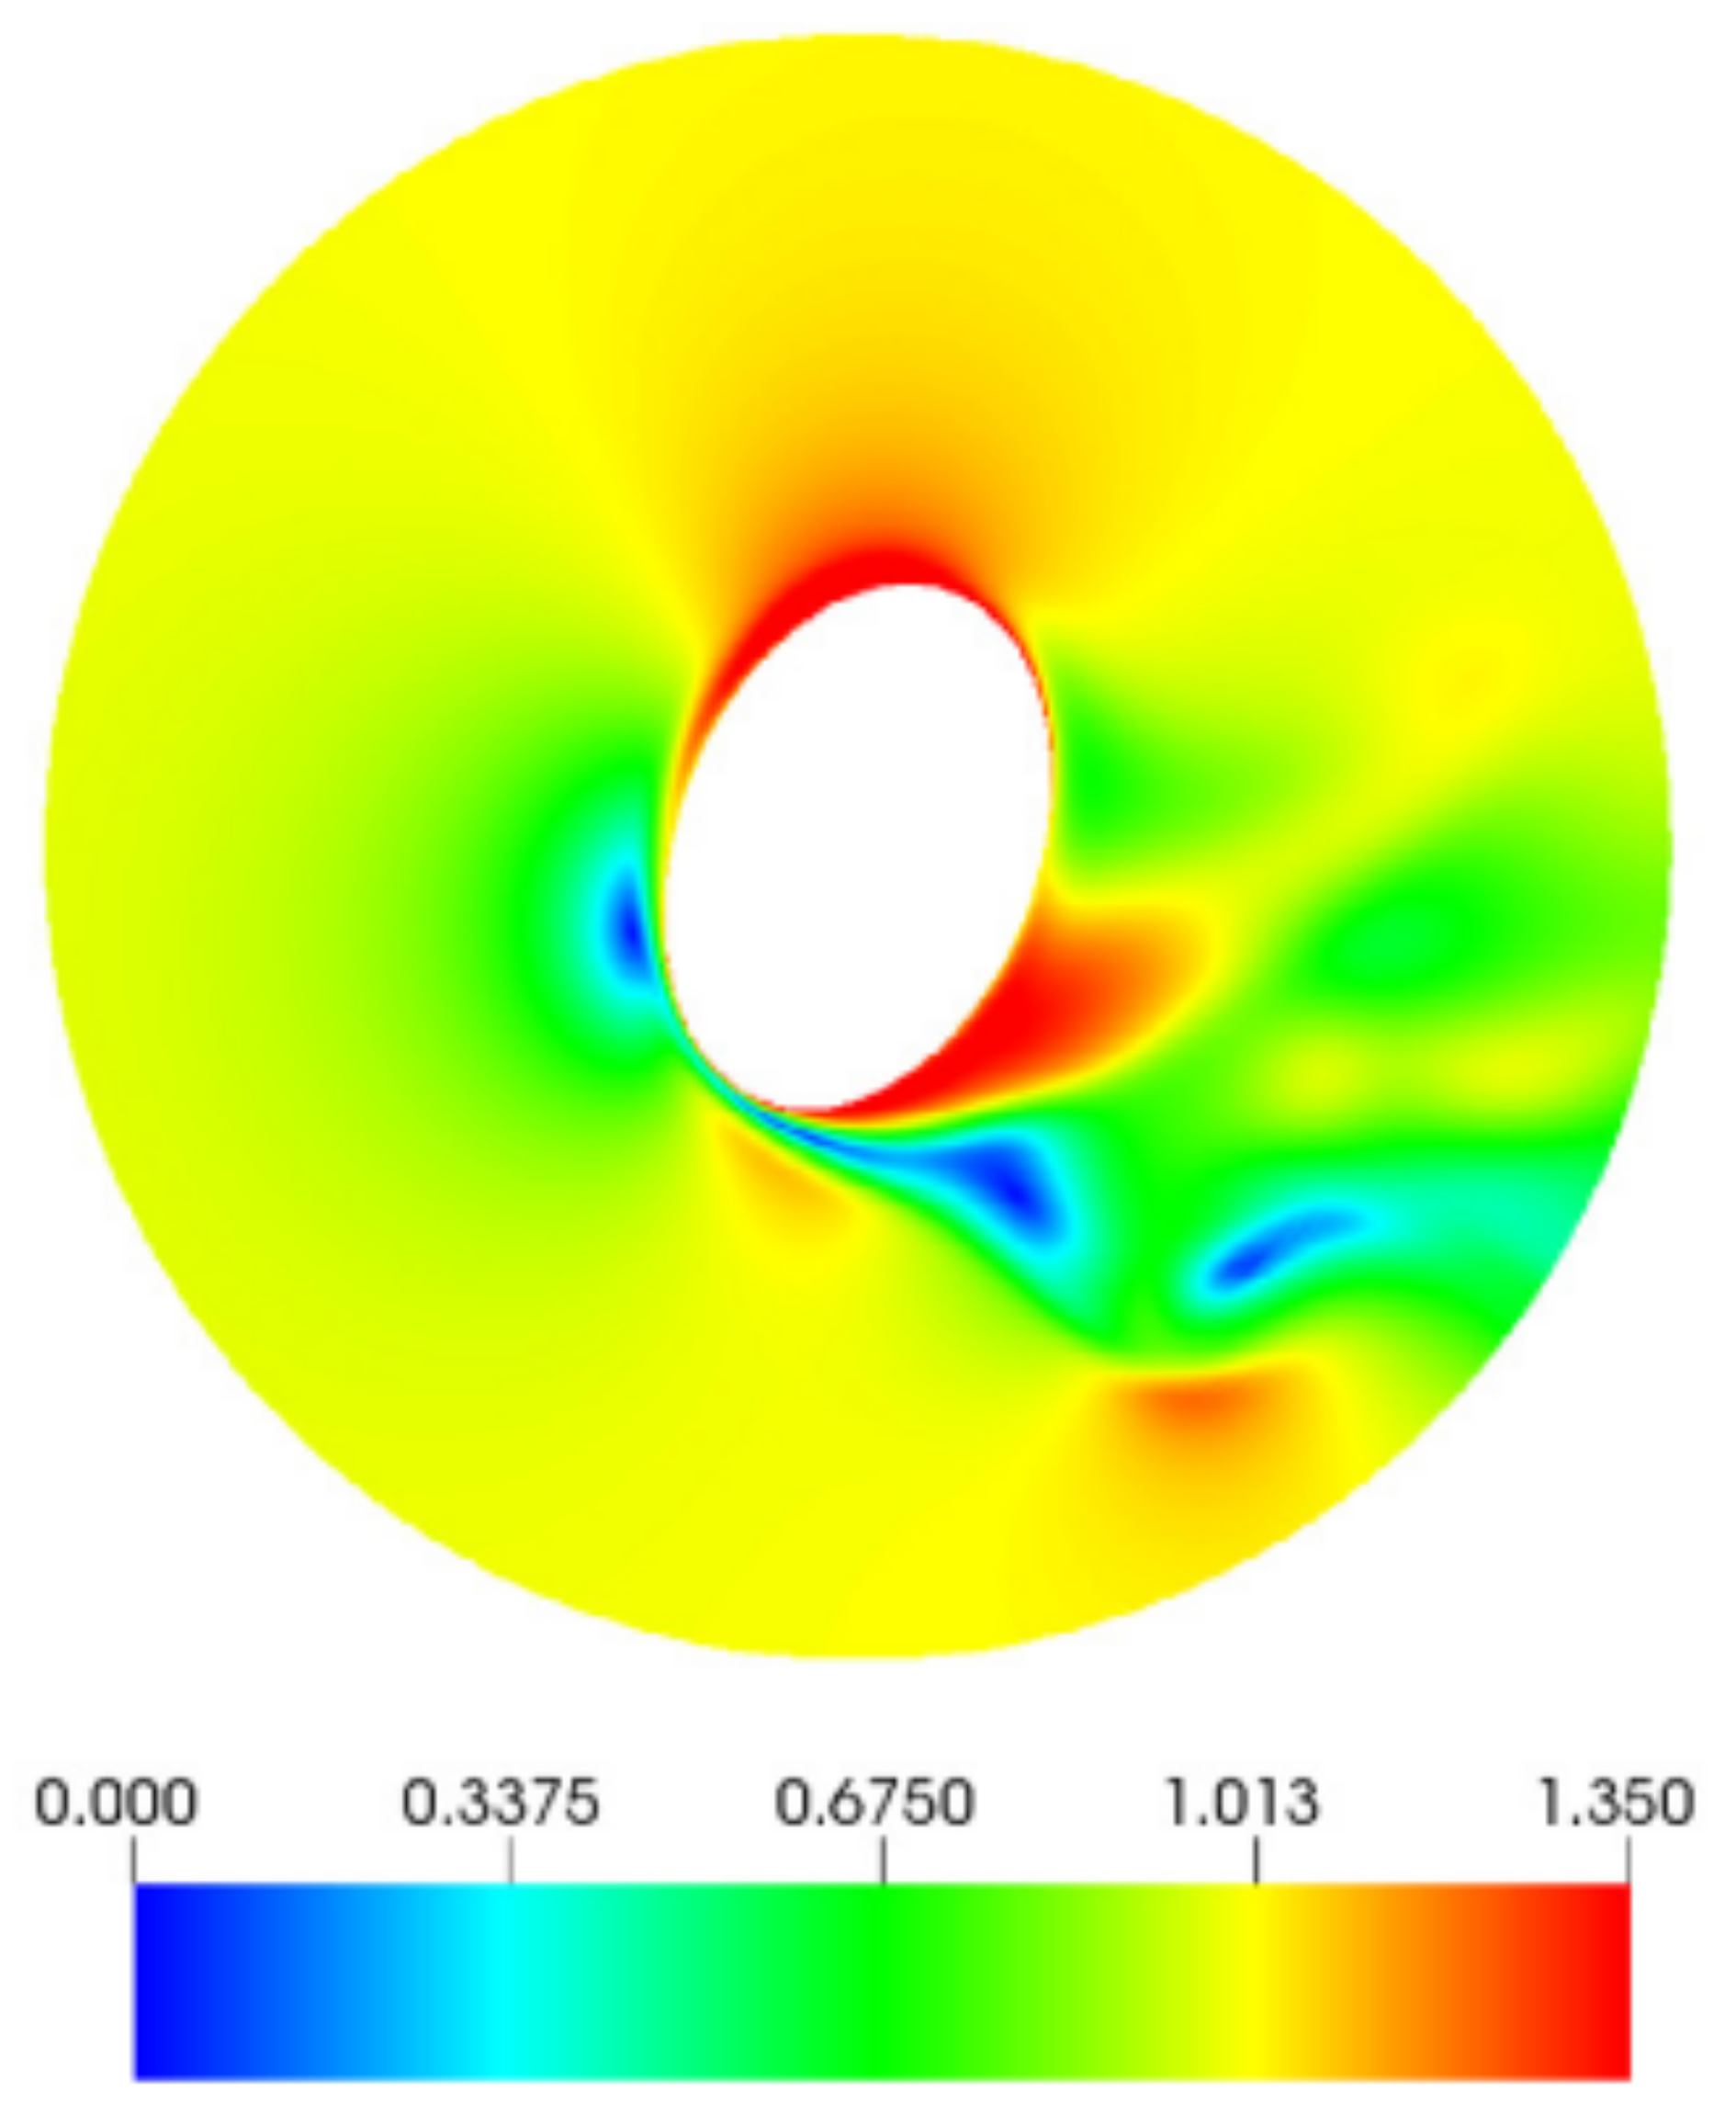
\includegraphics[width=.4\textwidth]{ams.png}
\caption{Velocity magnitude plot showing fluid being "dragged" along with clockwise rotation of body \cite{mittal_direct_2020}}
\label{fig:ams}
\end{figure}

Mercier et al. \cite{mercier_reflection_2008} perform an in-depth analysis solely dedicated to IGW. They transform the field data of a stratified medium by performing a Hilbert transformation. This consists of taking Fourier transforms, appling band-pass filtering, and then applying inverse Fourier transforms to 2D fields. They are able to obtain amplitude fields and frequency fields. They also obtain wavenumber fields in both directions. They are able to look at the behavior of the waves in the two different directions through the two waves numbers the transformation produces. They demonstrate the utility of this transformation by showing images in which different spatial wave numbers are filtered. The analysis they perform is used to deduce that backreflection of IGW off boundaries does not exist, which had originally been an assumption. Linear viscous theory of internal waves is also in good agreement with their results. In this study, an oscillating cylinder and a novel internal wave generator are utilized for IGW generation. These methods for generating IGW are substantially different from our spheriods of interest. 

Work by Fernando et al. is considered foundational in the field of bluff-bodies submerged in stratified flow. They run experiments of a nonrotating, horizontal cylinder in a stratified flow inside a tank. They ran experiments in the parameter space of $\{2000 \leq \Rey \leq 6000, 0.81 \leq Fr^2 \leq  169.0\}$. They investigate the effects these two parameters have on turbulent wake size and other structures. A paper that draws on the work of Fernando et al. is that of Deng et al. \cite{deng_drag_2022} who conducted numerical simulations of setups similar to Fernando et al. This study is one of the few to look at drag of bodies in stratified flows. They applied the Bousinesq approximation in their simulations, in which effects of stratification are only considered in the forcing portion of the Navier-Stokes equations. They show how high stratification ($Fr^2 \approx 0.02$) substantially increases drag, as Fig. \ref{fig:deng} shows. This is a result of the upstream blocking that occurs. This study also looks at the empirical stability parameter, $k$. This parameter is a function of $Fr^2$ and $\Rey$, and it estimates if there will be vortex-shedding. They found that $k$ behaves similarly to the drag coefficient at $Fr^2 \in (.25, 1)$.

\begin{figure}[htbp]
\centering
\includegraphics[width=0.7\textwidth]{deng.png}
\caption{Pressure distribution around cylinder at $Fr^2 = .0196$, $Re = 76$ \cite{deng_drag_2022}}
\label{fig:deng}
\end{figure}

Research by Ortiz et al. \cite{ortiz-tarin_stratified_2019} is among the first to look at translating nonrotating spheroids in stratified mediums by conducting 3D simulations using the finite-difference method . Their research looks at bodies of an aspect ratio ($AR$) of 4 at $\Rey = 10^4$. They compare a homogeneous case and three cases in the range $Fr^2 \in \{9, 1, 0.25\}$. Their analysis scrutinizes the effect of $Fr^2$ on IGW by observing y-velocity plots and showing stratification creates periodic semi-circular patters in the flow, which Fig. \ref{fig:sarkar} shows. They state that IGW are primarily caused by interactions with body itself, wake turbulence, and the coherent structures the body releases. A dominating effect they identify is the 3D horizontal movement of fluid around the body due to vertical confinement. They show some interesting plots of the lines of flow separation behind the body. At $Fr^2 = \infty$, the line is just a circle. As stratification increases, the separation line becomes elliptical, and then becomes more complicated. This analysis does not incorporate the effects of rotation.

\begin{figure}[htbp]
\centering
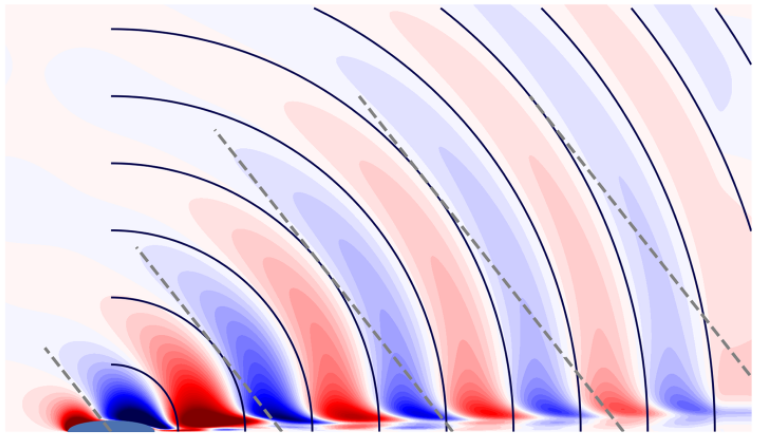
\includegraphics[width=0.7\textwidth]{sarkar.png}
\caption{Periodic semi-circular IGW patterns in vertical velocity at $Fr^2 = 1$ \cite{ortiz-tarin_stratified_2019}}
\label{fig:sarkar}
\end{figure}

Lu et al. \cite{lu_flow_2018} and Lua et al. \cite{lua_rotating_2018} conduct a parameter sweep of 2D spinning ellipses at $\Rey = 200$ in a homogeneous flow across different rotation rates. They vary their aspect ratios from 0.0625 to 1.0, find that at $AR \approx 0.5$, $\Omega^{\ast} > 2.0$, the body produces a thrust larger than the drag it experiences. Overall, they find that higher angular velocity $\Omega^{\ast}$ results in higher lift magnitude and lower drag. They attribute this thrust to a flow feature they call a "hovering vortex" with a center of low pressure. The hovering vortex exerts a force that pulls the body towards it. If the hovering vortex is in front of the body, it generates thrust. If the hovering vortex is behind the body, it generates drag.  

There has been a recent study conducted by Wang et al. \cite{wang_numerical_2023} looking at the behavior of a nonspherical, rotating body in stratified cross-flow. They conduct numerical simulations at $\Rey = 1000$ of a pitching airfoil, with the objective to fill the gap in knowledge in the field of flapping-foil flow energy harvester performance in stratified flows. They imposed the heaving (vertical translation) and pitching (rotation) motions of the airfoil. They simulated scenarios in the range of $Fr^2 \in [1, 100]$, along with some very high $Fr^2$ cases and $Fr^2 = \infty$ cases. They find that maximum energy extraction efficiency $\eta$ occurred in homogeneous flows. The value of $\eta$ has a decreasing trend as $Fr^2$ decreases until $Fr^2 = 16$. At that point, $\eta$ decreases substantially to an overall minimum at $Fr^2 = 4$. The value of $\eta$ increased through $Fr^2 = 1$. The power generation is dominated by the heaving motion at $Fr^2 > 2$, and by the pitching motion at $Fr^2 < 2$. The phenomenon behind the decrease in heaving power with decrease in $Fr^2$ is the disappearance of the leading-edge vortex (LEV), which can be attributed vertical confinement. This LEV plays a significant role in synchronicity between the heaving motion and heaving velocity; synchronicity is key to energy extraction efficiency. In the regime where pitching motion dominates energy extraction, the flow is dominated by IGW which create favorable conditions for increasing torque. The IGW dominate other features at high stratification. 

These studies have utilized lower-fidelity methods. Mittal et al. have developed and utilized an novel method known as the Schwarz-spectral element method (Schwarz-SEM) in the code Nek5000. This method was first validated in their 2019 \textit{Computers and Fluids} paper \cite{mittal_nonconforming_2019} where they show you can simulate flow around complex geometries with multiple overlapping meshes that exchange data. In their 2020 paper in the same journal, Mittal et al. applied this same method to 3D spinning spheroids in homogeneous flows \cite{mittal_direct_2020}. They validated their spinning sphere cases with results of spinning spheres in literature. They found that rotation angles of maximum drag and lift did not coincide with rotation angles of maximum frontal area and lateral area, as Fig. \ref{fig:mittal2020} shows. They also found that changing the aspect ratio of a spinning spheroid also changes the drag and lift forces acting on the body. They concluded that it is not possible to fully capture the flow features around a rotating body without explicitly modeling the solid-body rotation of the body.  

\begin{figure}[htbp]
\centering
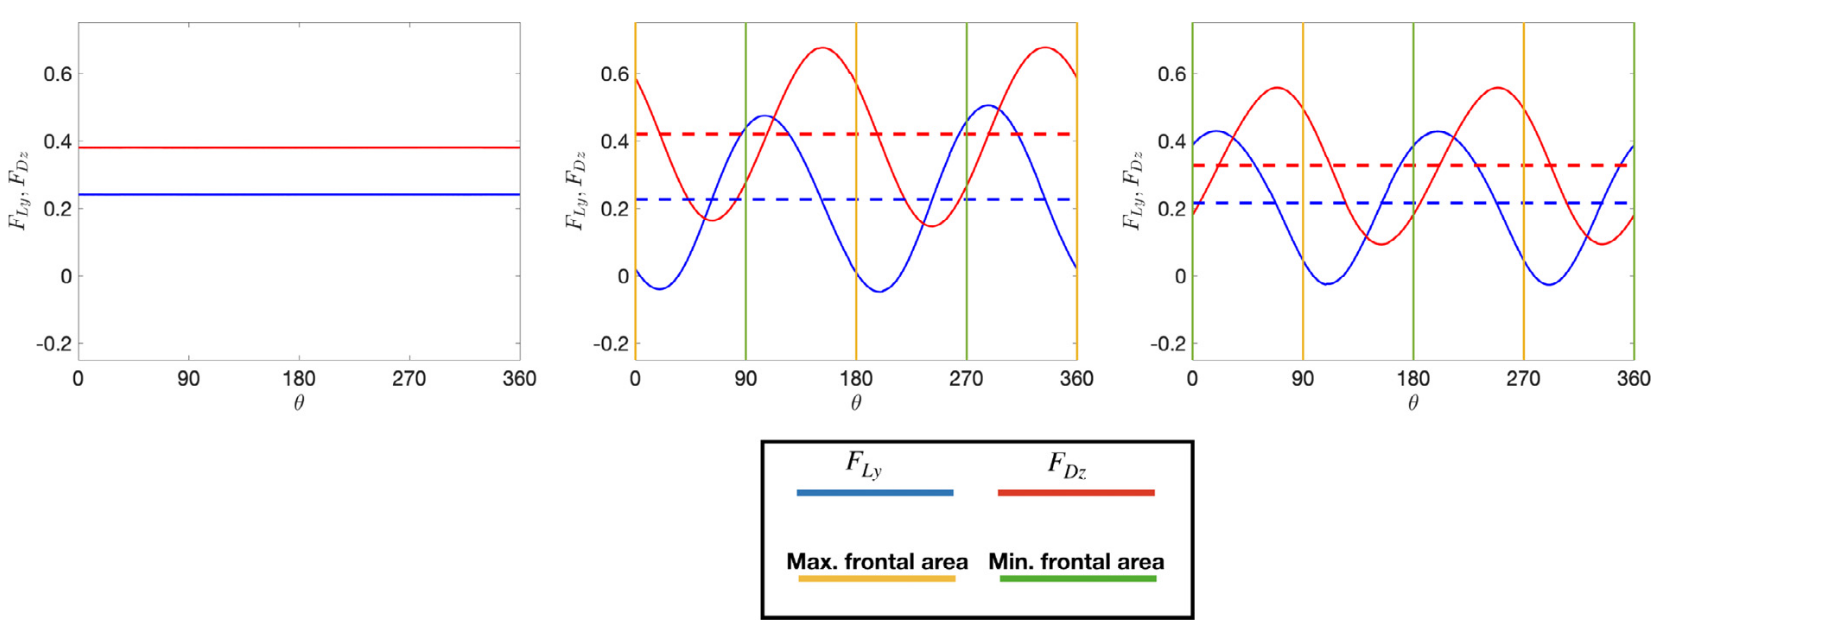
\includegraphics[width=\textwidth]{mittal2020.png}
\caption{Rotation phase difference in drag and lift \cite{mittal_direct_2020}}
\label{fig:mittal2020}
\end{figure}

The rest of this paper is divided into three chapters. In \hyperref[chp:Objectives]{Chapter 2} we discuss the goals for this research project, and in \hyperref[chp:Approach]{Chapter 3} we discuss the approach for meeting the goals we set in \hyperref[chp:Objectives]{Chapter 2}. In \hyperref[chp:Results]{Chapter 4} we show the results we have so far. 
\\

%\begin{figure}[htbp]
%\centering
%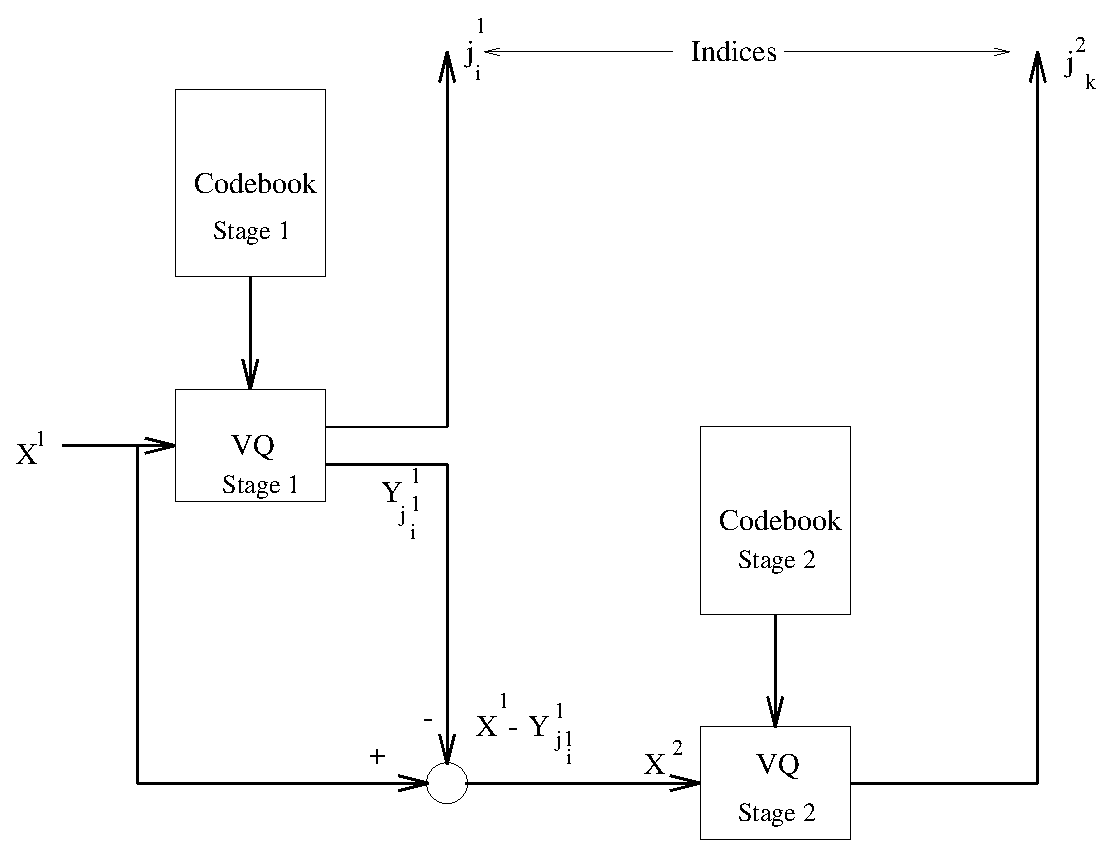
\includegraphics[width=0.7\textwidth]{samplefig}
%\caption{Binary splitting.}
%\label{fig:split}
%\end{figure}
%This figure is generated using an open-source figure drawing package
%(called {\tt fig}).  Any figure drawing package can be used to
%generate figures.  The easiest format for output is to output the
%figures in {\tt .pdf} format for inclusion in the {\tt .tex} file.
%
%% For the following three examples, note the problems with the xdvi
%% viewer described in the thesis.tex and the README.txt files.
%
%%%%%%%%%%%%%%%%%%%%%%%%%%%%%%%%%%%%%%%%%%%%%%%%%%%%%%%%%%%%%%%%%%%
%% TikZ example:  This is the same as the above figure, except done
%% using TikZ.
%%%%%%%%%%%%%%%%%%%%%%%%%%%%%%%%%%%%%%%%%%%%%%%%%%%%%%%%%%%%%%%%%%%
%\begin{figure}[!t]
%	\begin{center}
%		\begin{tikzpicture}[every text node part/.style={align=center}]
%			% Place nodes:
%			\draw (0,0) node[draw] (book1) {{\em Codebook}\\ {\small Stage 1}};
%			\draw ($(book1) + (0,-2)$) node[draw] (vq1) {{\em VQ}\\ {\small Stage 1}};
%			\draw ($(vq1) + (3,-3)$) node[circle,draw,minimum height=1cm] (adder) {$\Sigma$};
%			\draw ($(adder) + (5,0)$) node[draw] (vq2) {{\em VQ}\\ {\small Stage 2}};
%			\draw ($(vq2) + (0,2)$) node[draw] (book2) {{\em Codebook}\\ {\small Stage 2}};
%			
%			% Draw arrows:
%			\draw [-latex] (book1.south) -- (vq1.north);
%			\draw [-latex] (book2.south) -- (vq2.north);
%			\draw [-latex] ($(vq1.north east)+(0,-.25)$) node(vqout1) {} -| ($(adder.north)+(0,6)$) node[anchor=south west] (ji) {$j_i$};
%			\draw [-latex] ($(vq1.south east)+(0,.25)$) node(vqout2) {} -| (adder.north);
%			\draw [-latex] (vq1.west) -- ($(vq1.west)+(-1,0)$) node (in) {} |- (adder.west);
%			\draw [-latex] (vq2.east) -| ($(ji.south west) + (7,0)$) node[anchor=south west] (jk2) {$j_k^2$};
%			\draw ($(vq1.west)+(-2,0)$) node[anchor=east] {$X^1$} to[short,o-*] (in);
%			\draw [-latex] (in) -- (vq1.west);
%			\draw [-latex] (adder.east) -- (vq2.west);
%			
%			% Draw remaining labels:
%			\draw (vqout2) node[anchor=north west] {$Y_{j_i^1}^1$};
%			\draw (adder.north) node[anchor=south east] {$-$};
%			\draw (adder.west) node[anchor=south east] {$+$};
%			\draw (adder.east) node[anchor=south west] {$X^1-Y_{j_i^1}^1$};
%			\draw (vq2.west) node[anchor=south east] {$X^2$};
%			
%			% Draw annotation:
%			\draw ($(ji)!0.5!(jk2) + (0,1)$) node (indices) {\Large Indices};
%			\draw[thick,-triangle 45] (indices.west) to [out=180,in=45] (ji.north east);
%			\draw[thick,-triangle 45] (indices.east) to [out=0,in=135] (jk2.north west);
%		\end{tikzpicture}
%		\caption{Binary splitting (drawn with TikZ).}
%		\label{fig:split_tikz}
%	\end{center}
%\end{figure}
%
%%%%%%%%%%%%%%%%%%
%% CircuiTikZ example:
%%%%%%%%%%%%%%%%%%
%\begin{figure}[!t]
%	\begin{center}
%		\begin{tikzpicture}
%			\draw (0,0) node[op amp,scale=0.75] (oa){};
%			\draw (oa.out) to[short, -*] ++(1,0) node (n1) {};
%			\draw (n1.base) -- ++(1,0) to[C,l^=$C_S$,v_=$V_{\textrm{\small out,ofs}}$] ++(3,0) 	node[anchor=west] (n4) {$V_{\textrm{\small out}}$};
%			\draw (oa.-) to[short,-*] ++(-1,0) node (n2) {};
%			\draw (n2.base) |- ++(1,2) to[C] ++(2,0) -| (n1.base);
%			\draw ($(oa.+)+(0,-3)$) node[ground] {}  to[vsource=$V_{\textrm{\small in,ofs}}$] (oa.+);
%			\draw (n2.base) to[C] ++(-2,0) node[anchor=east] (n3) {$V_{\textrm{\small in}}$};
%		\end{tikzpicture}
%		\caption{Circuit example drawn using circuitikz.}
%		\label{fig:circuitikz_exmple}
%	\end{center}
%\end{figure}
%
%There are many other ways to create figures.  One package compatible
%with \LaTeX\ is TikZ.  An example is given in
%Fig.~\ref{fig:split_tikz}. This is identical to Fig.~\ref{fig:split},
%except that it is done within the compiling process of \LaTeX.
%Another example of a third-party figure package is given in
%Fig.~\ref{fig:circuitikz_exmple}.  This circuit was generated using
%the {\tt circuitikz} package.
%
%It is important that there is no text between figures when they are
%referenced close together in the text.  They should be ``stacked''
%without text in between as seen above.
%
%A final way of creating graphs is to use a open-sourse package called
%{\tt PGFPlots}.  An example of a good-looking graph generated using
%this package is given in Fig~\ref{fig:pgfplots_example}.  Note that
%this figure is large enough that it is pushed by \LaTeX\ to another
%page by itself and nicely centered.
%%%%%%%%%%%%%%%%%%
%% PGFplots example:
%%%%%%%%%%%%%%%%%%
%\begin{figure}[tbh]
%\begin{center}
%\begin{tikzpicture}
%\begin{semilogyaxis}
%[% 
%scale only axis, 
%width=5in, 
%height=5in, 
%xmin=0, 
%xmax=0.21, 
%xtick={0, 0.04, ..., 0.2},
%ymin=1e-006, 
%ymax=1, 
%yminorticks=true, 
%%xlabel={$\text{Tx Pulse amplitude }(\si{\volt})$},
%xlabel={Tx Pulse amplitude (V)},
%ylabel={Bit Error Probability}, 
%xmajorgrids, 
%ymajorgrids, 
%yminorgrids,
%legend columns=3,
%legend style={at={(0.5,-0.1)},anchor=north},%{at={(0.5,-0.5)},anchor=south},
%cycle multi list={%
%   color list\nextlist
%   [3 of]mark list}
%]
%
%%%%%%%%%%%%%%%%%%%%%%%%%%%%%%%%%%%%%%%%%%%%%%%%%%%%%%%%%%%%%%%%%%%
%%8p_NF4_uncoded
%\addplot [ color=blue, solid, mark=*, mark options={fill=blue} ] 
%coordinates{  
%(0.001,0.478052)(0.011,0.272706)(0.021,0.124776)(0.031,0.045402)(0.041,0.013449)(0.051,0.003469)(0.061,0.00094)(0.071,0.000328)(0.081,0.00017)(0.091,0.000108)(0.101,7.9e-005)(0.111,6e-005)(0.121,5.4e-005)(0.131,4.4e-005)(0.141,3.7e-005)(0.151,3.6e-005)(0.161,3.2e-005)(0.171,3.1e-005)(0.181,2.7e-005)(0.191,2.6e-005)(0.201,2.5e-005)  
%    };
%\addlegendentry{Uncoded}
%
%%8p_NF4_hard
%\addplot [ color=red, line width=1pt,dashed, mark=*,  mark options={fill=red},]
%coordinates{  
%(0.001,0.499268)(0.011,0.377753)(0.021,0.122226)(0.031,0.01535)(0.041,0.001172)(0.051,7.3e-005)(0.061,5e-006)(0.071,0)  
%};
%\addlegendentry{Hard decoded}
%
%%8p_NF4_soft
%\addplot [ color=black, dotted, line width=1.25pt,mark=*, mark options={fill=black} ] 
%coordinates{  (0.001,0.49911)(0.011,0.352208)(0.021,0.065849)(0.031,0.002668)(0.041,6e-005)(0.051,1e-006)  
%};
%\addlegendentry{Soft decoded}
%
%%%%%%%%%%%%%%%%%%%%%%%%%%%%%%%%%%%%%%%%%%%%%%%%%%%%%%%%%%%%%%%%
%
%%%%%%%%%%%%%%%%%%%%%%%%%%%%%%%%%%%%%%%%%%%%%%%%%%%%%%%%%%%%%%%%%%%
%%8p_NF5_uncoded
%\addplot [ color=blue, solid, mark=diamond*, mark options={fill=blue} ]
%coordinates{  (0.001,0.480507)(0.011,0.294723)(0.021,0.1521)(0.031,0.065413)(0.041,0.023695)(0.051,0.007415)(0.061,0.002195)(0.071,0.000714)(0.081,0.000305)(0.091,0.000167)(0.101,0.000109)(0.111,8.4e-005)(0.121,6.8e-005)(0.131,5.6e-005)(0.141,4.7e-005)(0.151,4.2e-005)(0.161,3.8e-005)(0.171,3.4e-005)(0.181,3.2e-005)(0.191,3.1e-005)(0.201,2.9e-005)      };
%\addlegendentry{Uncoded}
%
%%8p_NF5_hard
%\addplot [ color=red, dashed, mark=diamond*, mark options={fill=red} ]
%coordinates{  (0.001,0.499279)(0.011,0.403647)(0.021,0.17325)(0.031,0.033326)(0.041,0.003852)(0.051,0.000361)(0.061,2.9e-005)(0.071,3e-006)(0.081,1e-006)        
%};
%\addlegendentry{Hard decoded}
%
%%8p_NF5_soft
%\addplot [ color=black, dotted, line width=1.25pt,mark=diamond*, mark options={fill=black} ]
%coordinates{  (0.001,0.499265)(0.011,0.385162)(0.021,0.113072)(0.031,0.008749)(0.041,0.000313)(0.051,1e-005)(0.061,0)  
%};
%\addlegendentry{Soft decoded}
%%%%%%%%%%%%%%%%%%%%%%%%%%%%%%%%%%%%%%%%%%%%%%%%%%%%%%%%%%%%%%%%
%
%%%%%%%%%%%%%%%%%%%%%%%%%%%%%%%%%%%%%%%%%%%%%%%%%%%%%%%%%%%%%%%%%%%
%%8p_NF6_uncoded
%\addplot [ color=blue, solid, mark=square*, mark options={fill=blue} ]
%coordinates{  (0.001,0.482503)(0.011,0.315407)(0.021,0.179759)(0.031,0.088806)(0.041,0.038068)(0.051,0.014303)(0.061,0.004914)(0.071,0.001661)(0.081,0.000644)(0.091,0.000297)(0.101,0.000177)(0.111,0.000122)(0.121,9.5e-005)(0.131,7.1e-005)(0.141,5.8e-005)(0.151,5.3e-005)(0.161,4.6e-005)(0.171,4.2e-005)(0.181,3.6e-005)(0.191,3.4e-005)(0.201,3.3e-005)       };
%\addlegendentry{Uncoded}
%
%%8p_NF6_hard
%\addplot [ color=red, dashed, mark=square*, mark options={fill=red} ]
%coordinates{
%(0.001,0.499326)(0.011,0.424875)(0.021,0.22663)(0.031,0.062807)(0.041,0.010536)(0.051,0.001333)(0.061,0.000145)(0.071,1.6e-005)(0.081,4e-006)(0.091,0)  
%};
%\addlegendentry{Hard decoded}
%
%%8p_NF6_soft
%\addplot [ color=black, dotted, line width=1.25pt,mark=square*, mark options={fill=black} ] 
%coordinates{  (0.001,0.499363)(0.011,0.411563)(0.021,0.169253)(0.031,0.02352)(0.041,0.001472)(0.051,7.3e-005)(0.061,3e-006)(0.071,0)      
%};
%\addlegendentry{Soft decoded}
%
%%%%%%%%%%%%%%%%%%%%%%%%%%%%%%%%%%%%%%%%%%%%%%%%%%%%%%%%%%%%%%%%
%
%\end{semilogyaxis}
%
%\end{tikzpicture}
%
%\caption{Example figure made with PGFplots. Originally created in Matlab, then exported using the Matlab2TikZ script (available from Matlab Central). Then pasted into the \LaTeX\ document and edited for style. \label{fig:pgfplots_example} }
%\end{center}
%\end{figure}



% For use with multiple-paper format, uncomment the fillowing:
% \pagebreak
% \bibliographystyle{IEEEtran}
% \bibliography{IEEEabrv,BibFile1}  % uses the references stored in BibFile1.bib for this chapter

% Local Variables:
% TeX-master: "newhead"
% End:

    %
%  This is an example of how a LaTeX thesis should be formatted.  This
%  document contains chapter 2 of the thesis.
%
%  Time-stamp: "[sample-chapter2.tex] last modified by Scott Budge (scott) on 2016-07-28 (Thursday, 28 July 2016) at 08:40:50 on goga.ece.usu.edu"
%
%  Info: $Id: sample-chapter2.tex 967 2016-07-28 15:33:29Z scott $   USU
%  Revision: $Rev: 967 $
% $LastChangedDate: 2016-07-28 09:33:29 -0600 (Thu, 28 Jul 2016) $
% $LastChangedBy: scott $
%

\chapter{Objectives}
\label{chp:Objectives}

\begin{enumerate}
	\item I will identify the physical effects that causes differences in drag, and use this knowledge to identify good lateral boundary conditions and domain height.
	\begin{enumerate}
		\item I will identify why drag results are different when the lateral boundary condition are symmetric versus periodic. 
		\item I will identify why drag results are different when the height of the domain changes. 
	\end{enumerate}
	\item I will validate Neknek and Schwarz-SEM framework for spinning ellipses in stratified flows.
	\begin{enumerate}
		\item I will validate framework for spinning ellipses in homogeneous flows with existing literature.
		\item I will validate this framework for static circles in stratified flows using a mono-domain simulation based on an well-know Nek5000 example.  		
	\end{enumerate}
	\item I will find the effect of stratification on flow around spinning bodies.
	\begin{enumerate}
		\item I will compare drag and lift values for bodies across different $Fr^2$.
		\item I will compare schlerien and y-velocity field plots of flow around bodies for different $Fr^2$.
	\end{enumerate}
	\item I will find the effect of spin on flow around circular cylinders in stratified flow.
	\begin{enumerate}
		\item I will compare drag and lift values for cylinders of $\Omega^{\ast} = 0, 1$ 
		\item I will compare schlerien and y-velocity field plots of flow around cylinders of $\Omega^{\ast} = 0, 1$ 
	\end{enumerate}
\end{enumerate}

    \chapter{Approach}
\label{chp:3_Approach}
To identify the right domain size and boundary conditions, I will conduct 2D spinning circle simulations at $\Omega^{\ast} = 1, 3$ with periodic and symmetric boundary conditions. The three different domain heights that will be tested are $40D, 80D, 120D$. The main purpose of the $\Omega^{\ast}=1$ cases is to find which boundary conditions and domain size satisfy our needs, since our parameter sweep will occur at $\Omega^{\ast}=1$. We will see at what domain size are the values of drag insensitive to changes in boundary conditions and domains height. The main purpose of the $\Omega^{\ast}=3$ cases is to identify the physics, since the effects will be obvious. We will plot the surface pressure distribution of the circles to see how the pressure distribution shifts. 

To validate the Schwarz-SEM (Neknek) framework for spinning ellipses, I will run simulations at $\Rey = 200$ of spinning ellipses of aspect ratios 0.5 and 1.0 at $\Omega^{\ast} = 1,2,3$ in homogeneous flow. I will compare the drag and lift values to those of \cite{lu_flow_2018} and \cite{lua_rotating_2018}.
\section{Governing equations {\&} problem setup}
\label{section:governing_equations_and_setup}
We want to ascertain the effect shape, spin, and stratification have on flow. We start by discussing how we account for stratification. We use the same setup used by \cite{fischer_nek5000_nodate} in the Nek5000 user guide. We relate the density $\rho$ at a given height $\mathbf{x}$ to the constant background density $\rho_0$, $\rho = \rho_0 + \rho ' (\mathbf{x},t)$. The term $\rho'$ is the perturbation density, which we will assume to have a linear profile. This means the overall density $\rho$ has a linear profile. To account for the buoyancy forces from stratification, we utilize the Boussinesq approximation. The Boussinesq approximation is where effects of density stratification are only applied to the forcing term, or terms multiplied by gravity forces in this case, in the governing equations. The Boussinesq approximation also assumes $\rho_0 \gg \rho '$.
We apply the Boussinesq approximation to the nondimensional Incompressible Navier-Stokes Equations (INSE) shown in Equations \ref{eq:INSE} and \ref{eq:cont}:

\begin{equation}
    \label{eq:INSE}
    \frac{\partial\mathbf{u}}{\partial t}+\mathbf{u}\cdot\nabla\mathbf{u}=-\nabla p+\frac{1}{\Rey}\nabla^2\mathbf{u}-\frac{1}{{Fr}^2} (\rho^\prime\ -\ y )\hat{y}
\end{equation}

\begin{equation}
    \label{eq:cont}
    \nabla \cdot \textbf{u} = 0
\end{equation}
We also solve the transport equation in \ref{eq:density transport}, which is the material derivative of the perturbation density set equal to a diffusion operator.  
\begin{equation}
    \label{eq:density transport}
    \frac{\partial\rho '}{\partial t}+\mathbf{u}\cdot\nabla\rho'=\frac{1}{\Pran \Rey}\nabla^2\rho '
\end{equation}
The three nondimensional numbers that appear in the equations above are defined as such:
\begin{equation}
    \Rey = \rho_0 \frac{U D}{\mu}, \Pran = \rho_0 \frac{\kappa}{\mu}, Fr^{-2}=\frac{gD^2}{\rho_0 U^2}|\rho^{\prime}_{y,0}|
\end{equation}
where $\rho^{\prime}_{y,0}$ is the density gradient, which in this case is constant. The term $U$ is the velocity scale, $D$ is the length scale, which will be discussed more later. Dynamic viscosity, also known as momentum diffusivity, is represented by $\mu$, and $\kappa$ is the diffusivity of the property that is causing the stratification, which in this case is thermal diffusivity. Because the densimetric Froude term $Fr^{-2}$ is slightly clunky, often it is substituted with the Richardson number $Ri \coloneqq Fr^{-2}$. We are able to extract the physical quantity called the Brunt–Väisälä frequency defined as
\begin{equation}
    \label{eq:NBV}
    N_{BV} \coloneqq \bigg( \frac{g}{\rho_0} \rho^{\prime}_{y,0} \bigg)^{1/2}    
\end{equation}
With nondimensionality and setting $U = 1$ and $D = 1$, the Brunt–Väisälä frequency can be redefined in terms of nondimensional parameters to yield
\begin{equation}
    \label{eq:nondim NBV}
    N_{BV} = Ri^{1/2} = Fr^{-1}
\end{equation}
We observe that with higher stratification, we get higher frequencies of oscillation. 
To understand the effect of shape, we look at three different aspect ratios. A circle is included to allow for benchmarking purposes with literature since a sufficient number of studies have looked at spinning circles. It is shown that the horizontal dimension, $a_x$ of the body is held constant, and this dimension is what is used for the length scale used in the Reynolds number $\Rey = \rho_0 \frac{U D}{\mu}$ , where $D = 2a_x$. The other dimension $a_y$ is varied to achieve the different aspect ratios. The aspect ratio is defined as $AR = a_y/a_x$. Figure \ref{fig:flow setup} show the aspect ratios of interest for this study. 
Now we introduce spin into our setup. We follow the conventions of \cite{mittal_direct_2020} and define our nondimensional rotational velocity as $\Omega^{\ast} = \tilde{\Omega}D/2 U_{\infty}$, where $\tilde{\Omega}$ is the rotational velocity in radians per unit time. Figure \ref{fig:flow setup} shows how the ambient flow, rotation, and axes are related. The axis of rotation, which in this case is the out-of-plane z-axis, is normal to the flow. The flow occurs in the x-direction. 
\begin{figure}
    \centerline{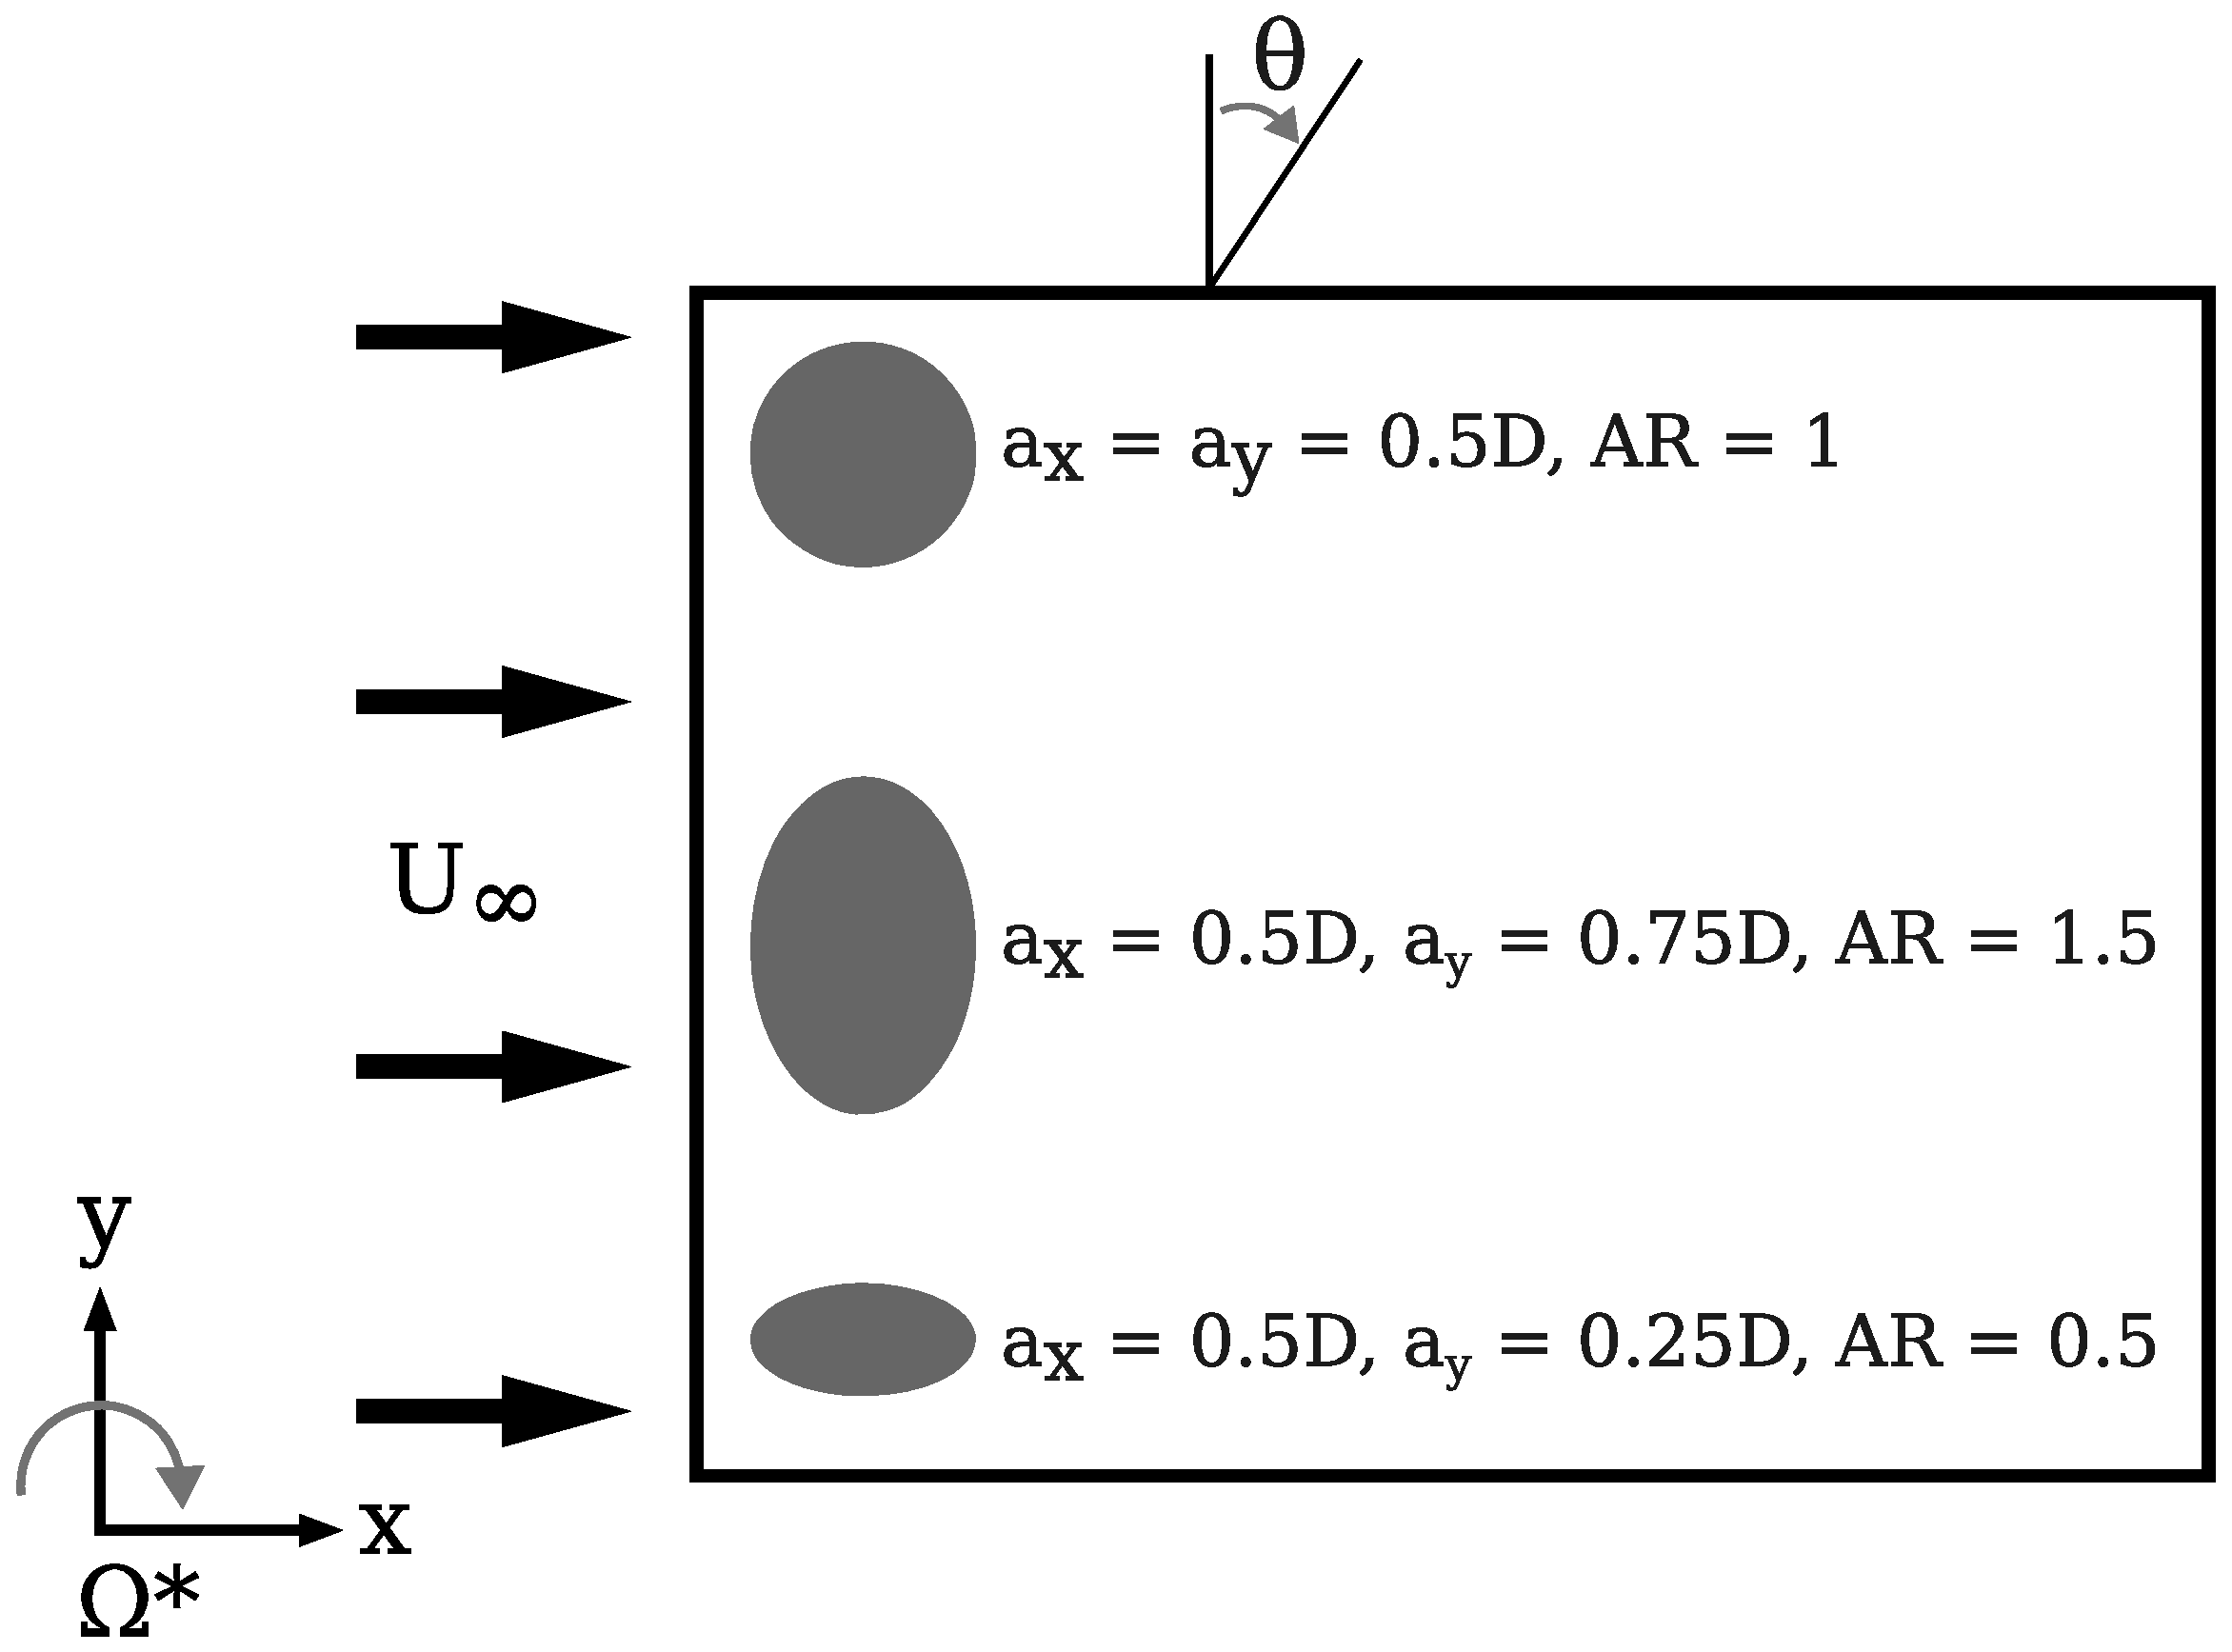
\includegraphics[width=.6\textwidth]{flow_setup.eps}}
    \caption{Schematic showing aspect ratios of interest}
    \label{fig:flow setup}
\end{figure}

This study utilizes Spectral Element Methods to perform DNS. These methods allow for higher-order accuracy than methods used in past studies. Lagrange interpolants with Gauss-Lobatto-Legendre (GLL) quadrature are utilized. 
We consider cases at $\Rey = 120$. We do not go much higher than $\Rey = 120$ because at $\Rey >190$ flow regimes, 2D simulations do not sufficiently capture the flow features observed in 3D simulations as stated by \cite{deng_drag_2022}. We do not want to go to smaller $\Rey$ because the flows of interest occur at $\Rey > 100$. We run simulations where the stratification is a result of a linear temperature distribution, and we run simulations at a constant $\Pran = 1$. The rates of rotation of interest we will consider are $\Omega^{\ast} = 0, 1$. We compare cases with spin and no spin to observe what effect introduction of spin has on the flow. Table \ref{table:parameter_space} give the values of our parameter sweep. A few simulations will be run outside this parameter space to explore transitional flow regimes. 
\begin{table}
  \centering
  \begin{tabular}{cc}
    Parameters      & Values   \\ \hline
    $AR$   & $0.5, 1.0, 1.5$ \\
    $Fr^2$ & $0.01, 0.1, 1.0, 10.0, 100.0, \infty$     \\
    $\Rey$ & $120$  \\
    $\Omega^{\ast}$ & $0.0$ (AR = 1 \text{only}), $1.0$  \\
  \end{tabular}
  \caption{The values of interest for our parameter sweep}
  \label{table:parameter_space}
\end{table}
 \clearpage

\section{Schwarz-SEM framework}
\label{section:schwarz-SEM_framework}
Because we intend to simulate nonspherical spinning bodies, it becomes necessary to create two different meshes. We create one circular mesh which conforms to the shape of the body and rotates with the body. We utilize another static, background mesh with a circular cavity where the circular mesh is placed. There is an overlap between the two meshes to allow for data exchange. We utilize the Schwarz-SEM framework, which allows us to run simulations with multiple meshes. The Schwarz-SEM framework has its roots in the Overlapping-Schwarz (OS) methods developed by Schwarz in 1870 \cite{mittal_nonconforming_2019}. Laplace's equation was solved on two overlapping domains by interpolating interdomain boundary conditions.  

\begin{figure}\centerline{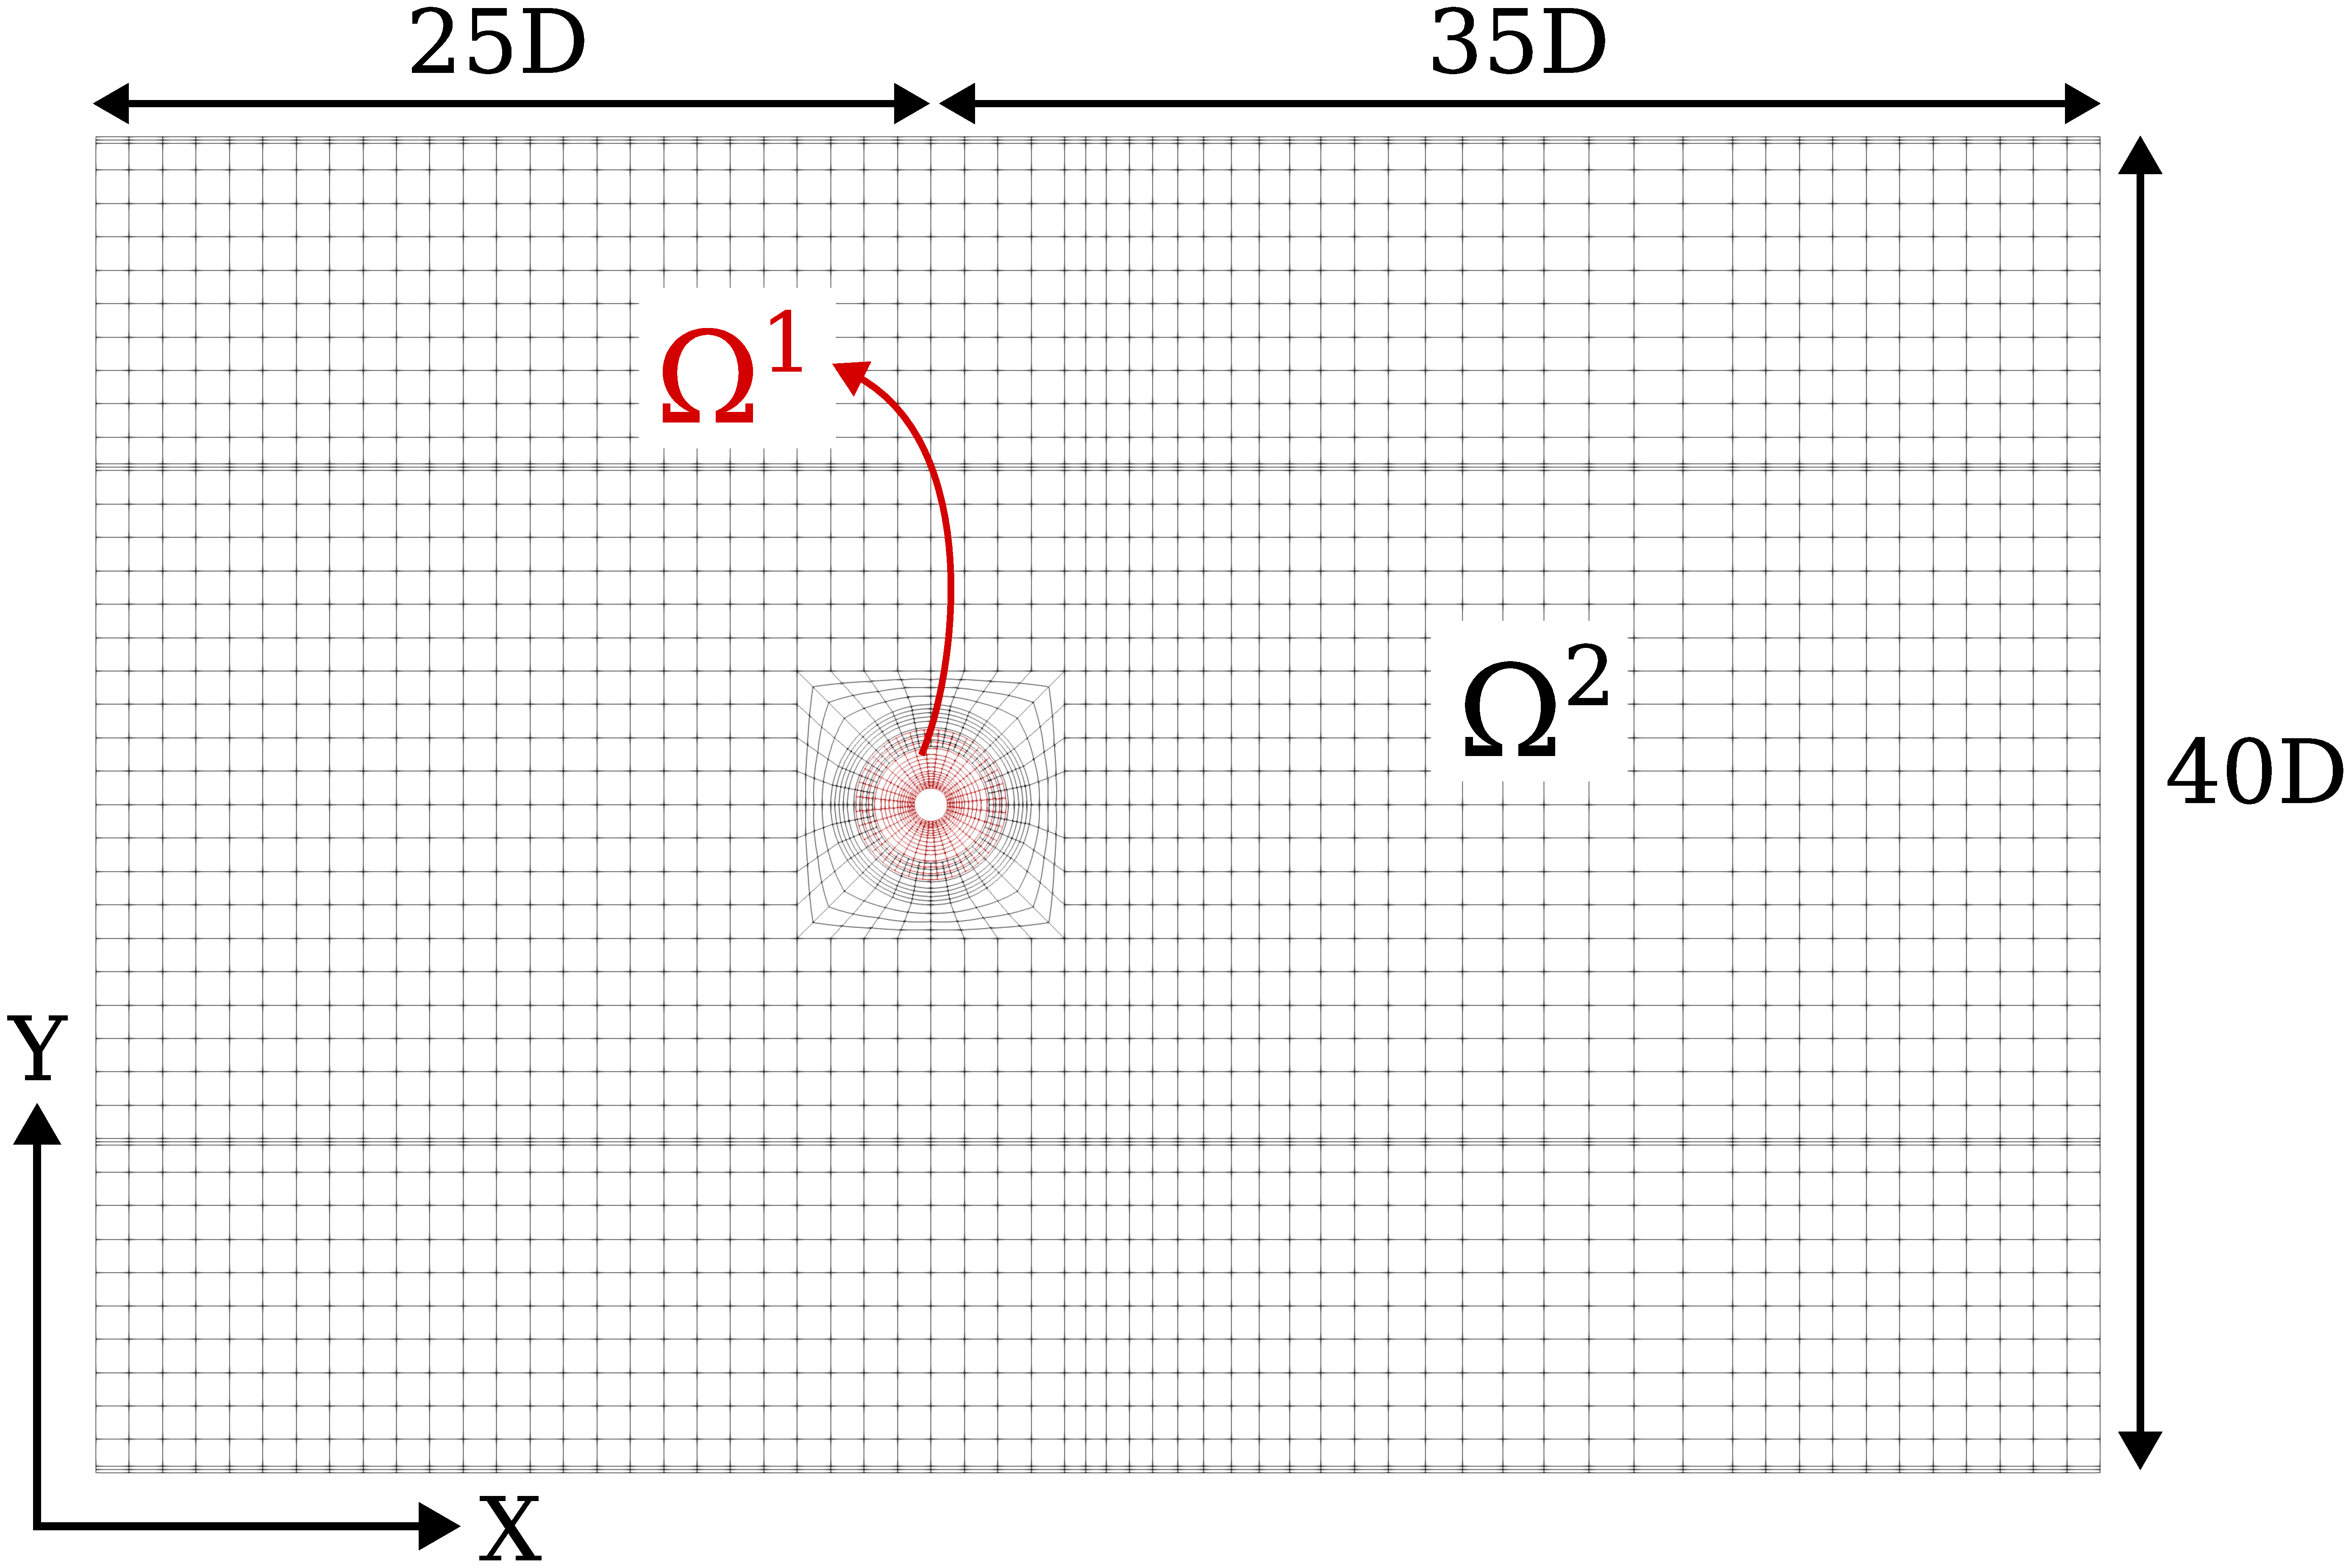
\includegraphics[width=.8\textwidth]{mesh.eps}}
    \caption{A figure showing the two meshes $\Omega^1$ and $\Omega^2$ in the Schwarz-SEM framework}
    \label{fig:mesh}
\end{figure}

In spite of the fact that the Schwarz-SEM framework was developed with the intention for use in static domains, an Arbitrary Lagrangian-Eulerian (ALE) formulation has been developed to allow for moving bodies. The implementation of the ALE formulation occurs with a modification of the convective term in Equations \ref{eq:INSE} and \ref{eq:density transport} as \cite{merrill_moving_2019} show. The advantage of using an overlapping mesh rather than a sliding mesh is we are able to retain spectral accuracy. Sliding mesh methods are limited to second-order accuracy.
For advancing in time, a semi-implicit scheme is implemented, rather than a fully implicit scheme. The reason for choosing a semi-implicit scheme is the cost of a fully implicit scheme as discussed by \cite{tomboulides_numerical_1997}. In the semi-implicit scheme, the nonlinear terms and Boussinesq forcing term are treated explicitly with \textit{k}th-order extrapolation since they would increase the cost substantially if treated implicitly. The time derivative is implicitly treated with a \textit{k}th-order backward difference formula (BDF\textit{k}) because we want to retain high-order temporal accuracy. The viscous and pressure terms are decoupled and treated implicitly through Poisson updates.\\\\
Every timestep, the boundary conditions at the interdomain boundaries are interpolated from the adjacent mesh. This occurs every timestep because the locations of the inner mesh GLL nodes change every timestep. \cite{mittal_nonconforming_2019} implemented a routine called \textit{findpts\_eval} from the library \textit{gslib} that carries out the boundary condition interpolation. Using the \textit{findpts} routine, the routine \textit{findpts\_eval} finds the corresponding element and element coordinates from the adjacent mesh.\\\\
At the interdomain boundaries, the solutions are advanced in time every timestep with EXT\textit{m} using $m$ number of preceding steps in time to increase the temporal accuracy. Higher order $m$ leads to instability, so $q$ corrector iterations are implemented every timestep, and the data is interpolated from the adjacent domain before every corrector iteration. In the case of our parameter sweep, we set $m=3$ and $q=5$ to achieve sufficient data exchange. \\\\  
The top and bottom boundaries have Neumann symmetric boundary conditions. The left boundary has a Dirichlet constant velocity inflow boundary condition, while the right boundary has a Neumann zero-pressure outflow boundary condition. Meanwhile, the surface of the cylinder has a Dirichlet no-slip wall boundary condition. The size of the domain is $60D \times 40D$, where $D$ is the length of the non-varying axis of the ellipse; the radius of the inner mesh is $2.25D$. The inner mesh consists of 512 elements, while the outer mesh consists of 3200 elements. There is an overlap of $0.5D$ between the meshes. 

\clearpage

\section{Validation}
\label{section:validation}
We start by validating our Schwarz-SEM framework against a commonly-used nonspinning circle monodomain SEM case. We ran monodomain and Schwarz-SEM simulations in domains of size 43x24. In these validation cases, our parameter space is $\{\Rey, \Pran, AR, \Omega^{\ast}\} = \{120, 1, 1, 0\}$. Figure \ref{fig:nn val} compares the drag coefficient, which is calculated as $C_D = 2F_D$. We only see a slight disagreement at $Fr^2 = 0.01$, which comes out to an error of less than $3.1\%$.  

\begin{figure}
    \centerline{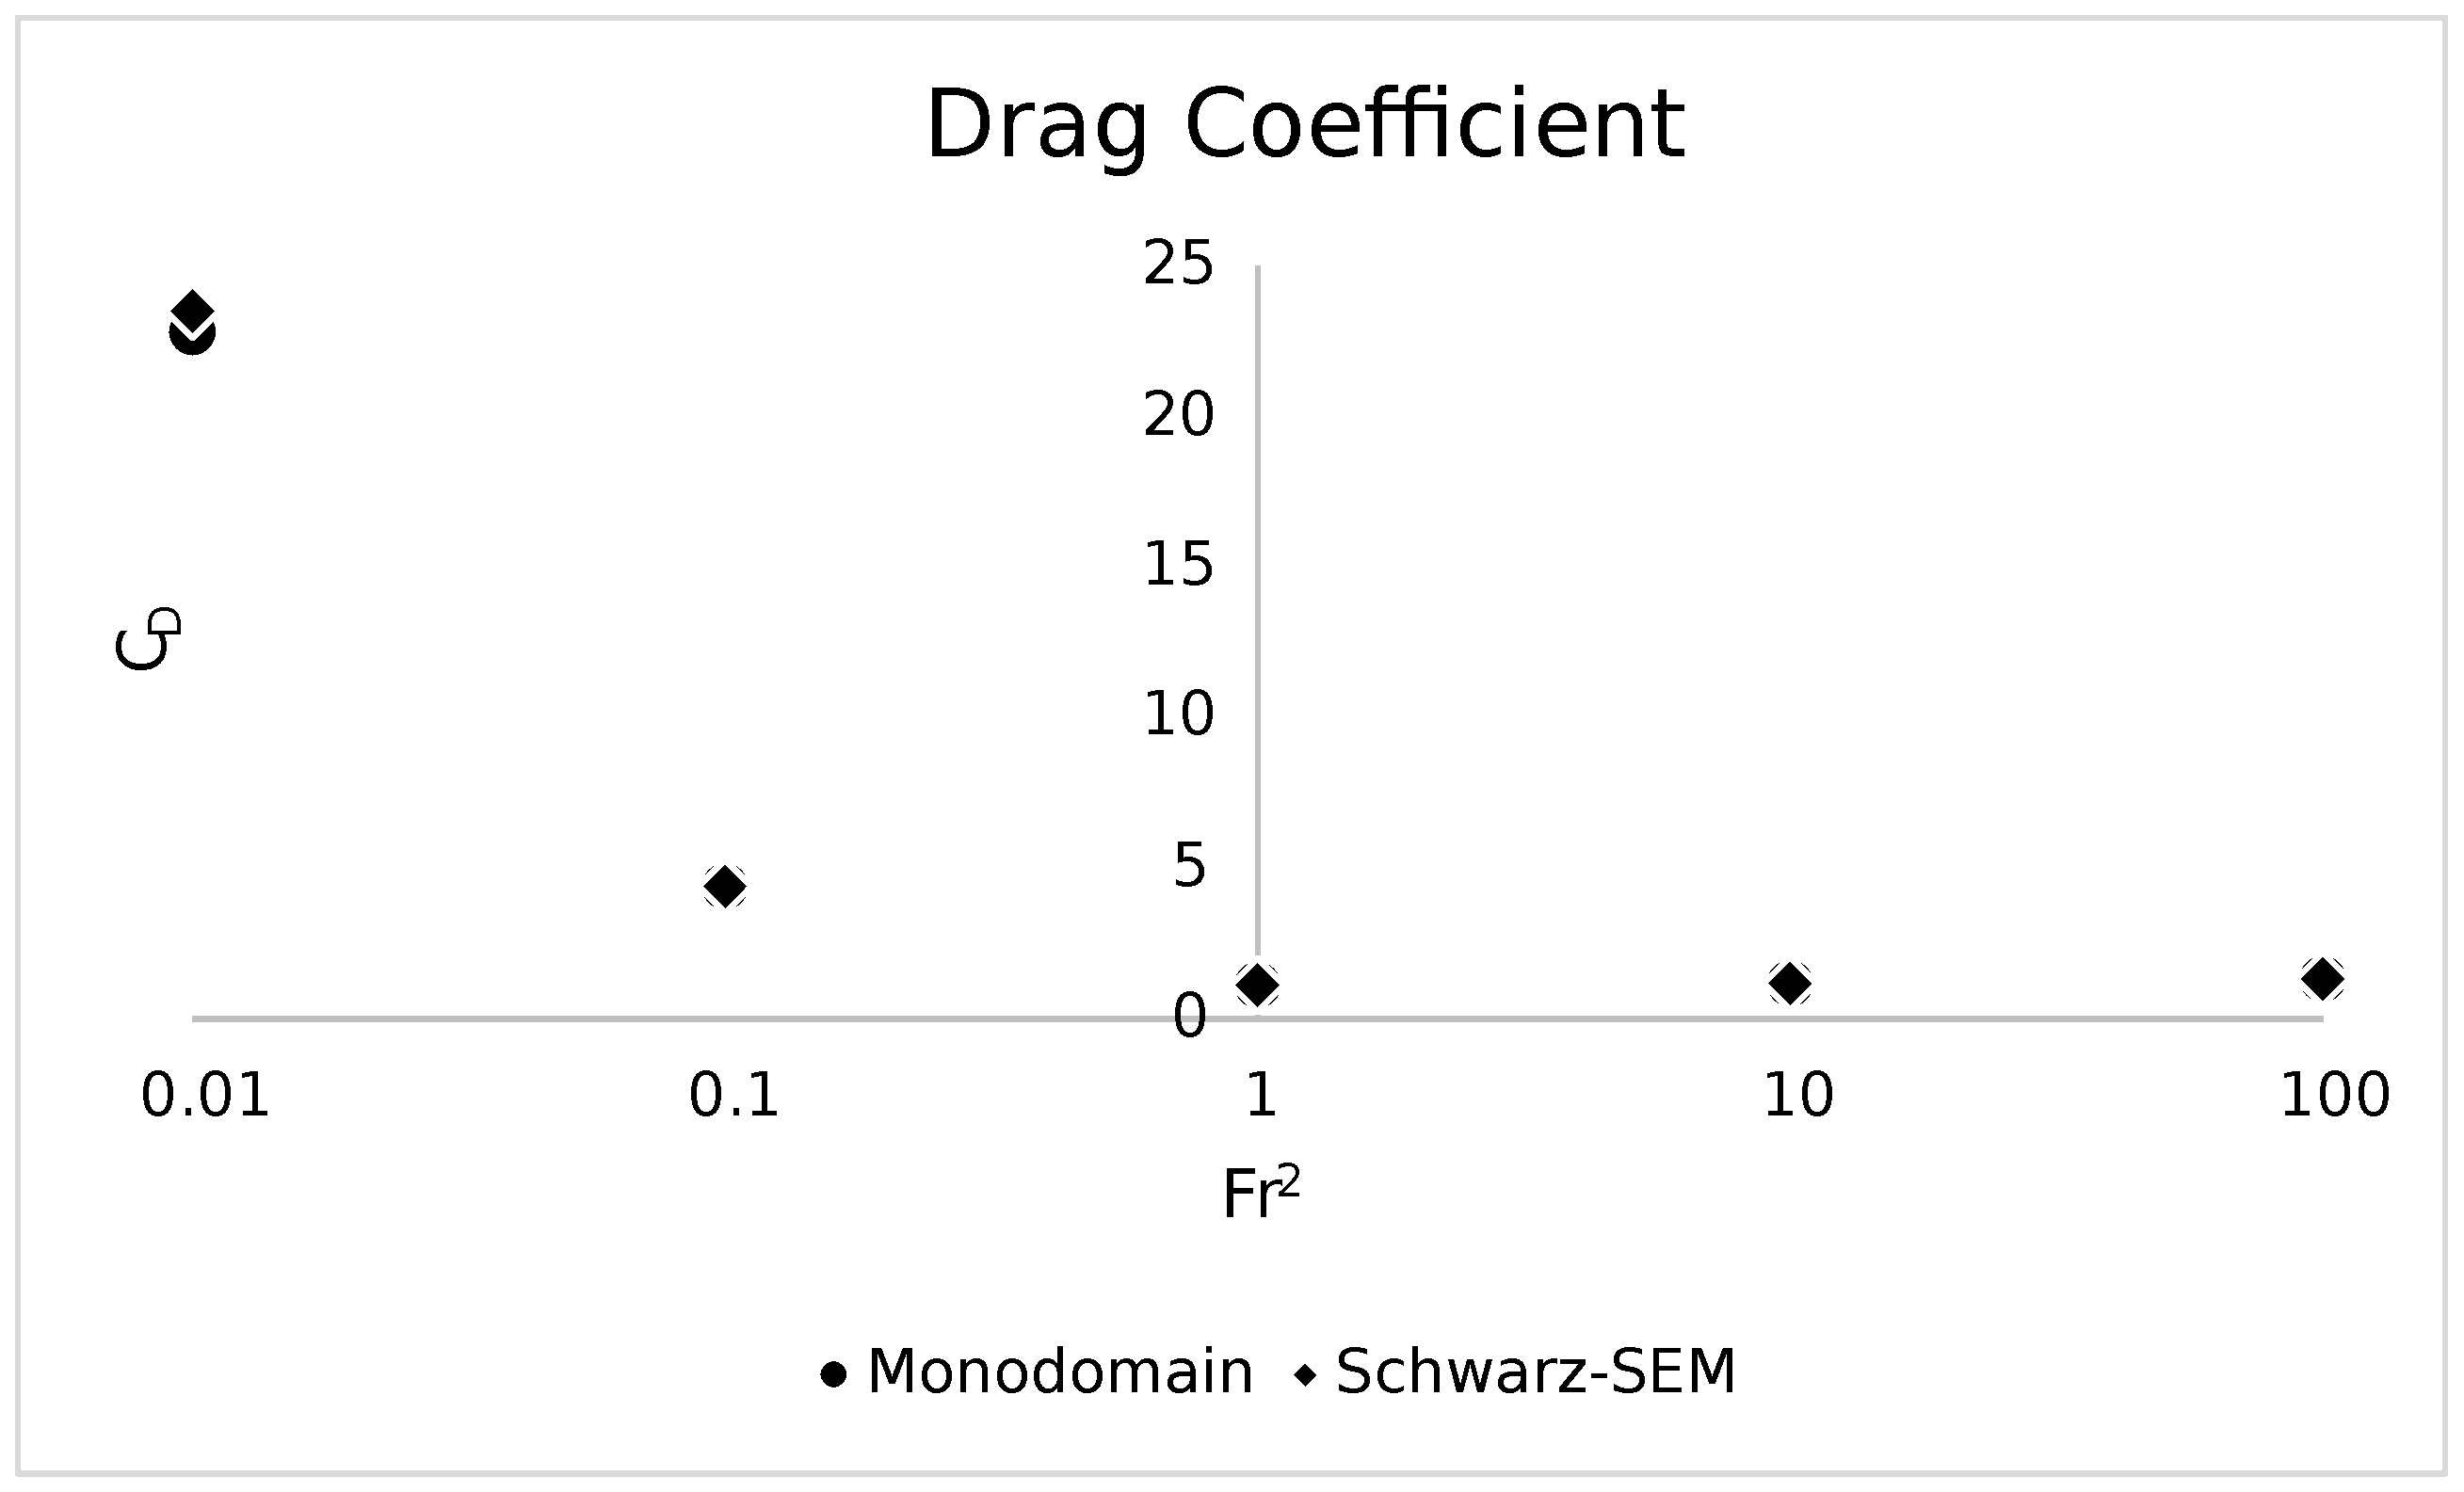
\includegraphics[width=.8\textwidth]{images/dragvalnn.eps}}
    \caption{Validation of the Schwarz-SEM framework at $\Omega^{\ast}$ for stratified flow}
    \label{fig:nn val}
\end{figure}

Now that the nonspinning stratified Schwarz-SEM for circular shapes has been validated, we move to validating the nonstratified, elliptical Schwarz-SEM framework. We compare our drag and lift results with those of two papers, Lu et al. \cite{lu_flow_2018} and Lua et al. \cite{lua_rotating_2018}. Our domain dimensions and boundary conditions matched. Figure \ref{fig:lua drag} shows the drag results between us and the two papers. Interestingly, the net thrust observed by the two papers is also observed in our results.
\begin{figure}
    \centering
    \begin{subfigure}{0.49\textwidth}
    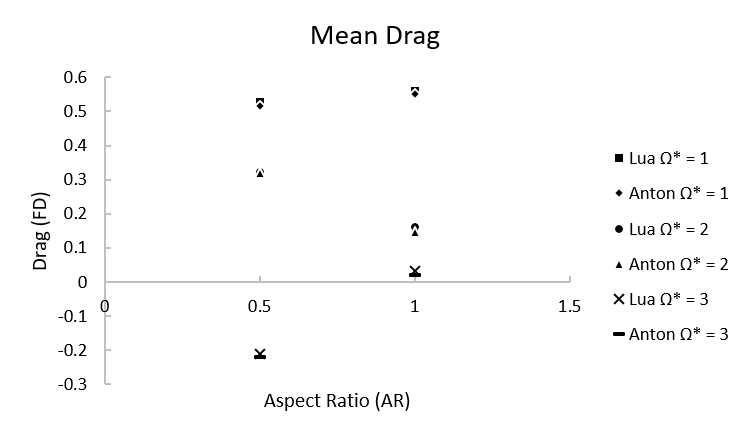
\includegraphics[width=\textwidth]{draglua.png}
    \caption{Comparison of drag results with Lua et al.}
    \label{fig:lua drag}
    \end{subfigure}
    \begin{subfigure}{0.49\textwidth}
    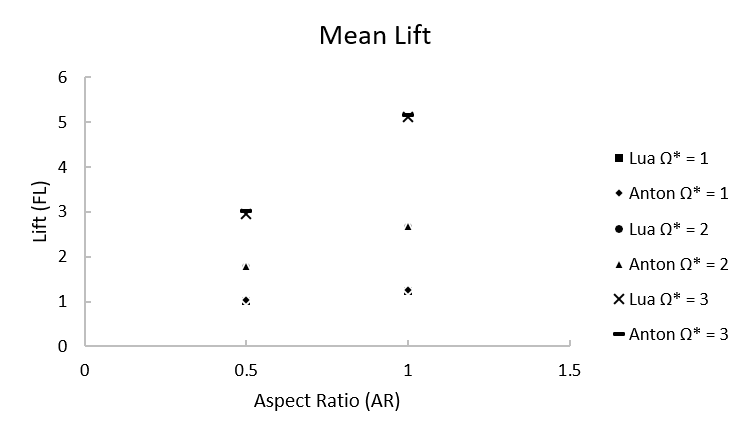
\includegraphics[width=\textwidth]{liftlua.png}
    \caption{Comparison of lift results with Lua et al.}
    \label{fig:lua lift}
    \end{subfigure}
    \caption{Comparison against Lua et al.}
    \label{fig:lua_com}
\end{figure}
While conducting these validation tests, it was found that at higher rotation rates, the drag values are more sensitive to domain size and lateral boundary conditions. This is a topic that is not discussed much in the literature; domain size and lateral boundary conditions are not given much consideration. 

Figure \ref{fig:domain_conv} shows that in the case of $\Omega^{\ast} = 3$, there is a large discrepancy in drag at height $H = 40D$ between the two boundary condition types. We also see that as we change the domain size, regardless of boundary condition, the drag also changes.  However, there is a vertical length of convergence for domain size. For the case of $\Omega^{\ast} = 3$, we observe a convergence towards a value of about $120D$. Interestingly, the variance is higher in the case of the periodic boundary conditions than the symmetric boundary conditions. The figure also shows that there is also a vertical length of convergence where the drag for the periodic and symmetric boundary condition cases converge. The required height increases with rotational velocity, as expected. 
\begin{figure}
    \centerline{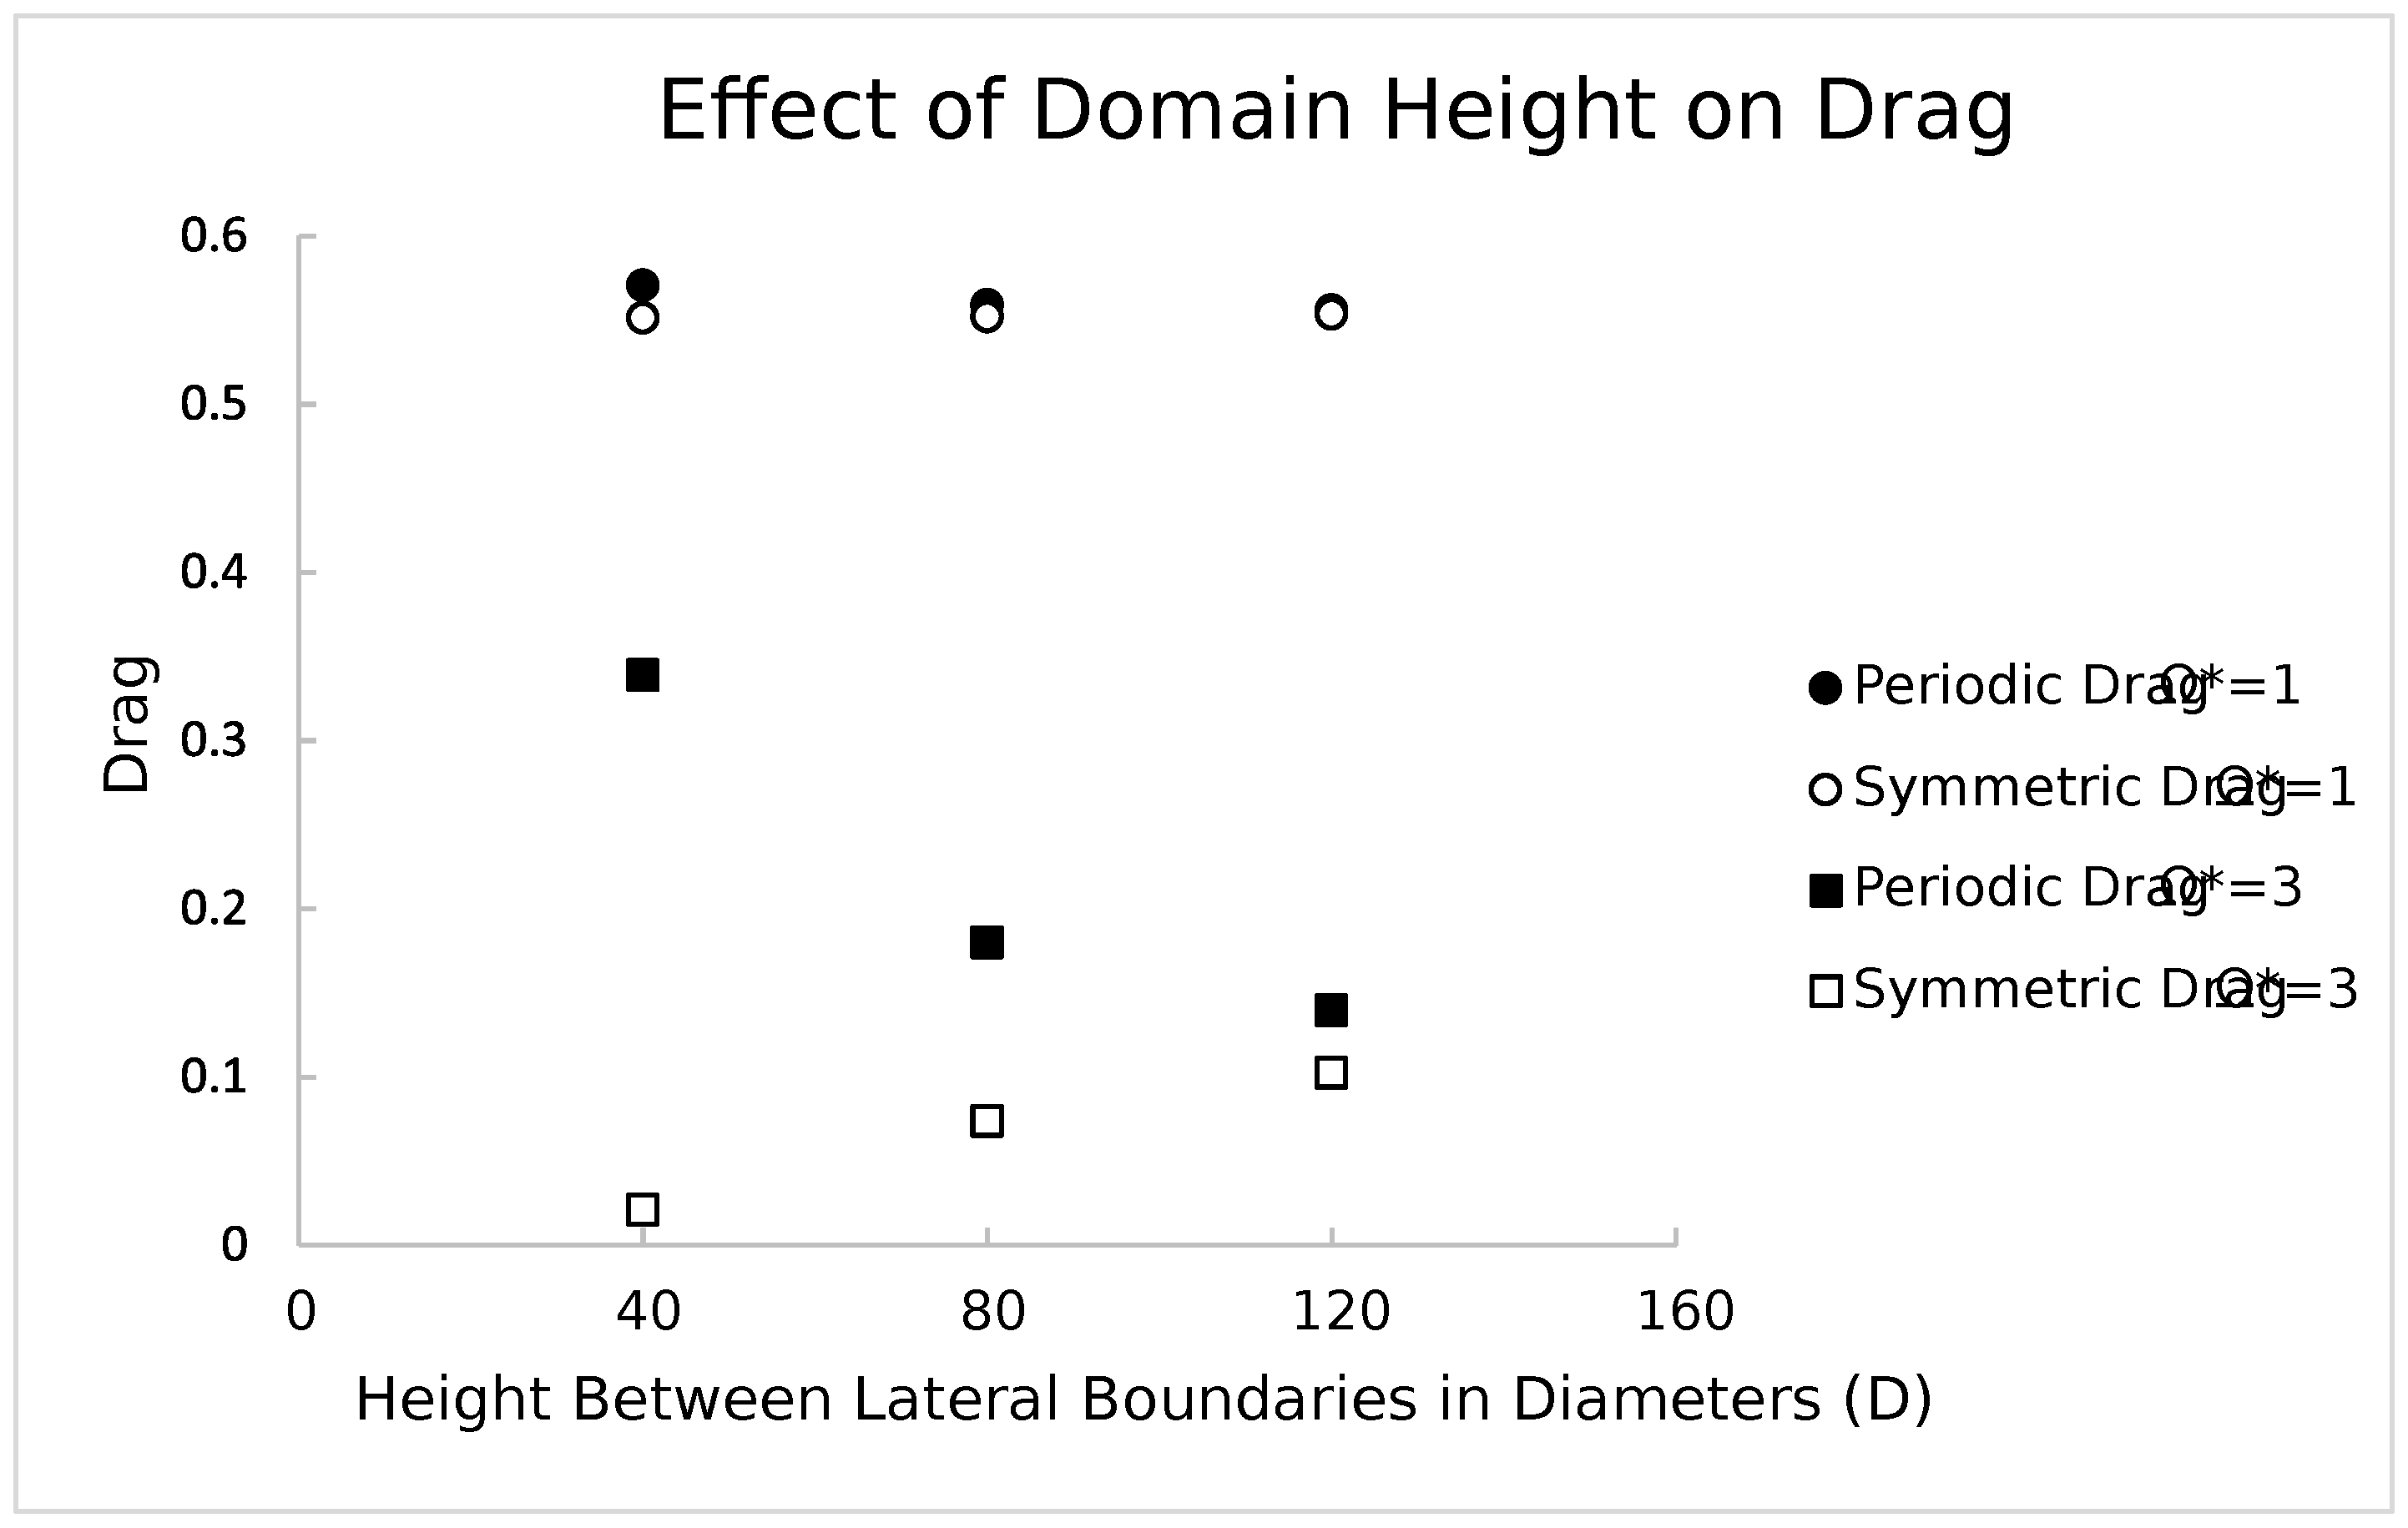
\includegraphics[width=.9\textwidth]{domain.eps}}
    \caption{At higher rotation speeds, larger domain sizes are required}
    \label{fig:domain_conv}
\end{figure}
In figure \ref{fig:per}, we see how in the case of the periodic boundary conditions, the rotation of the cylinder is able to redirect the flow down since the periodic boundary conditions allow for flow normal to the boundaries; the flow comes done from the top, further redirecting the flow. This does not happen in the case of the symmetric boundary conditions, as figure \ref{fig:sym} shows. Because there is no flow normal to the boundaries at the boundaries, there is no flow rotation like there is in the case of the periodic boundary conditions. 
\begin{figure}
    \centering
    \begin{subfigure}{0.49\textwidth}
    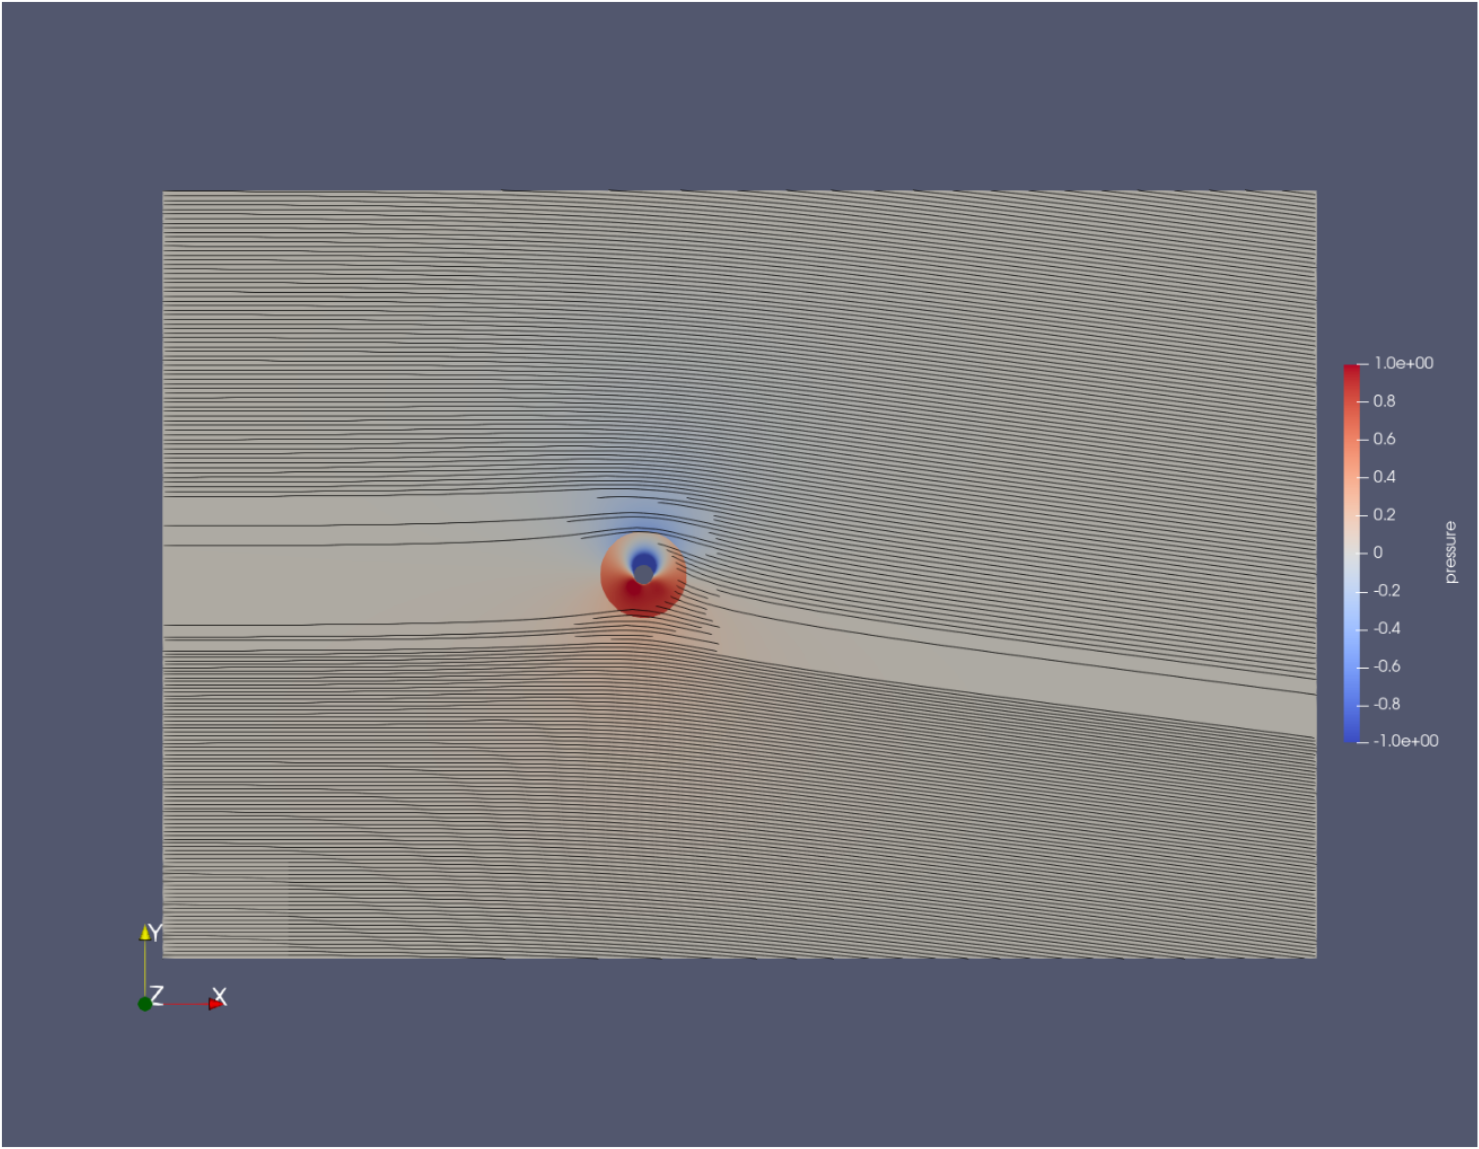
\includegraphics[width=\textwidth]{per.png}
    \caption{Periodic boundary conditions}
    \label{fig:per}
    \end{subfigure}
    \begin{subfigure}{0.49\textwidth}
    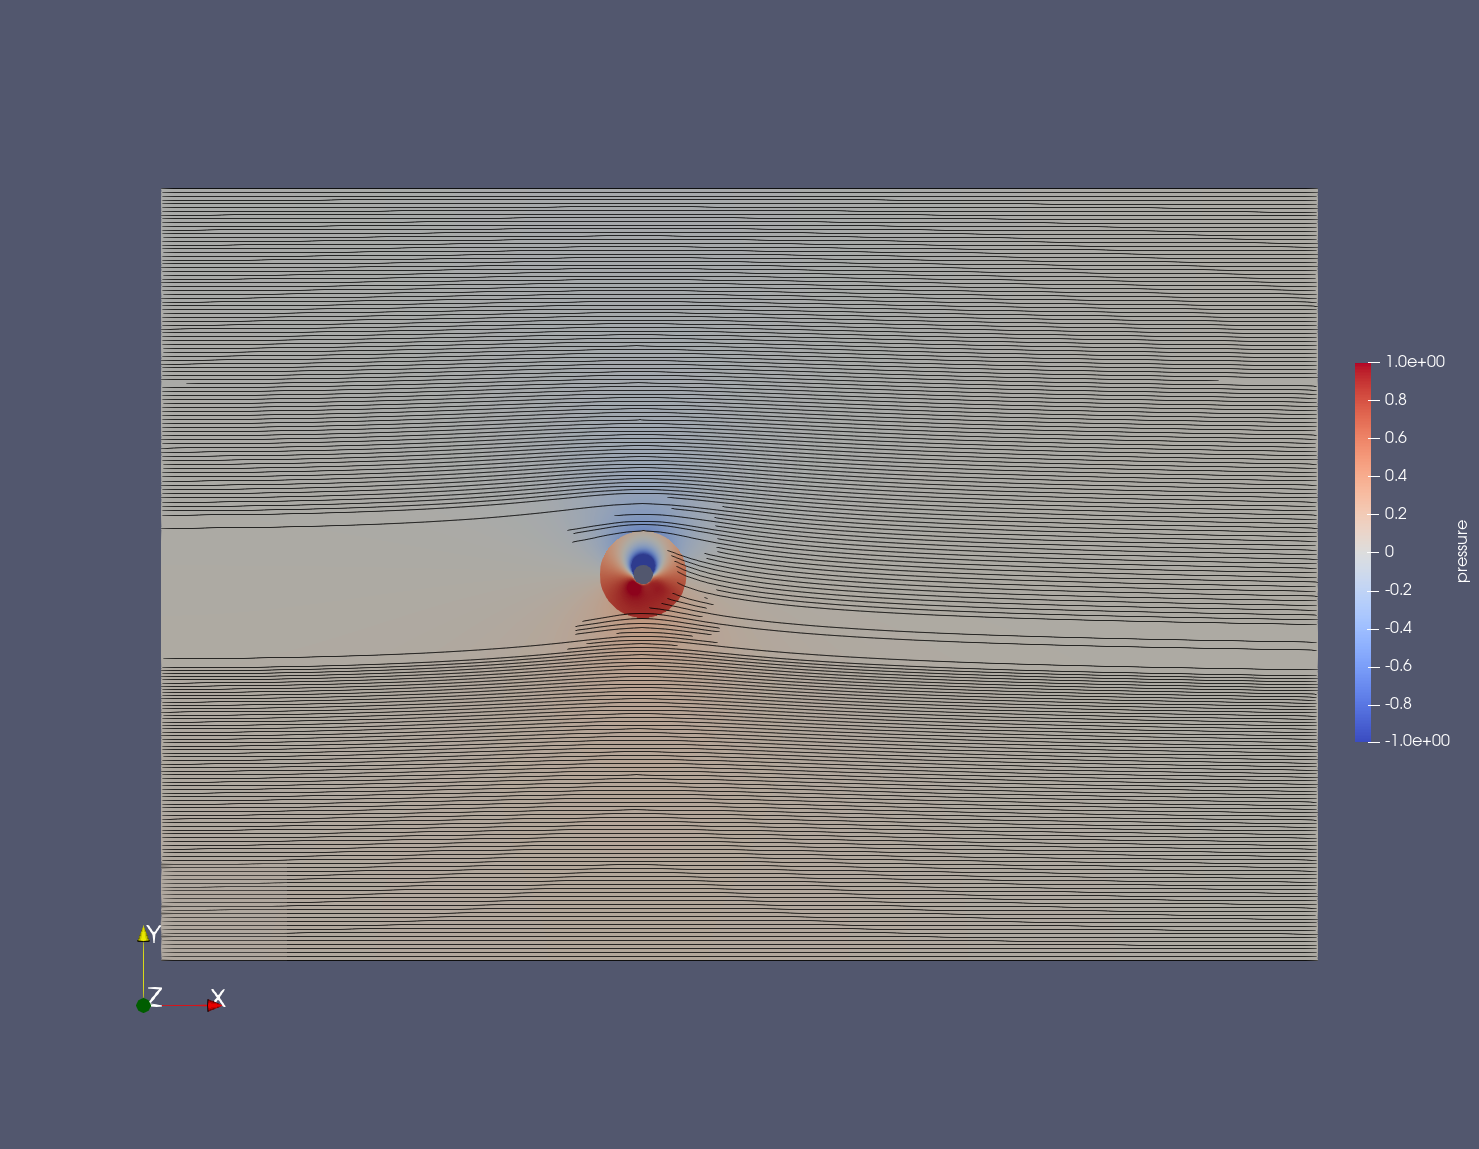
\includegraphics[width=\textwidth]{sym.png}
    \caption{Symmetric boundary conditions}
    \label{fig:sym}
    \end{subfigure}
    \caption{Pressure and streamline plots at $H = 40D$, $\Omega^{\ast} = 3$, $\Rey = 200$, aspect ratio = 1}
    \label{fig:per sym}
\end{figure}
The flow rotation in the case of the periodic boundary conditions also rotates the pressure distribution, as figure \ref{fig:polar pres} shows. The clockwise rotation of the negative pressure zone at the top creates a net increase in drag.
\begin{figure}
    \centerline{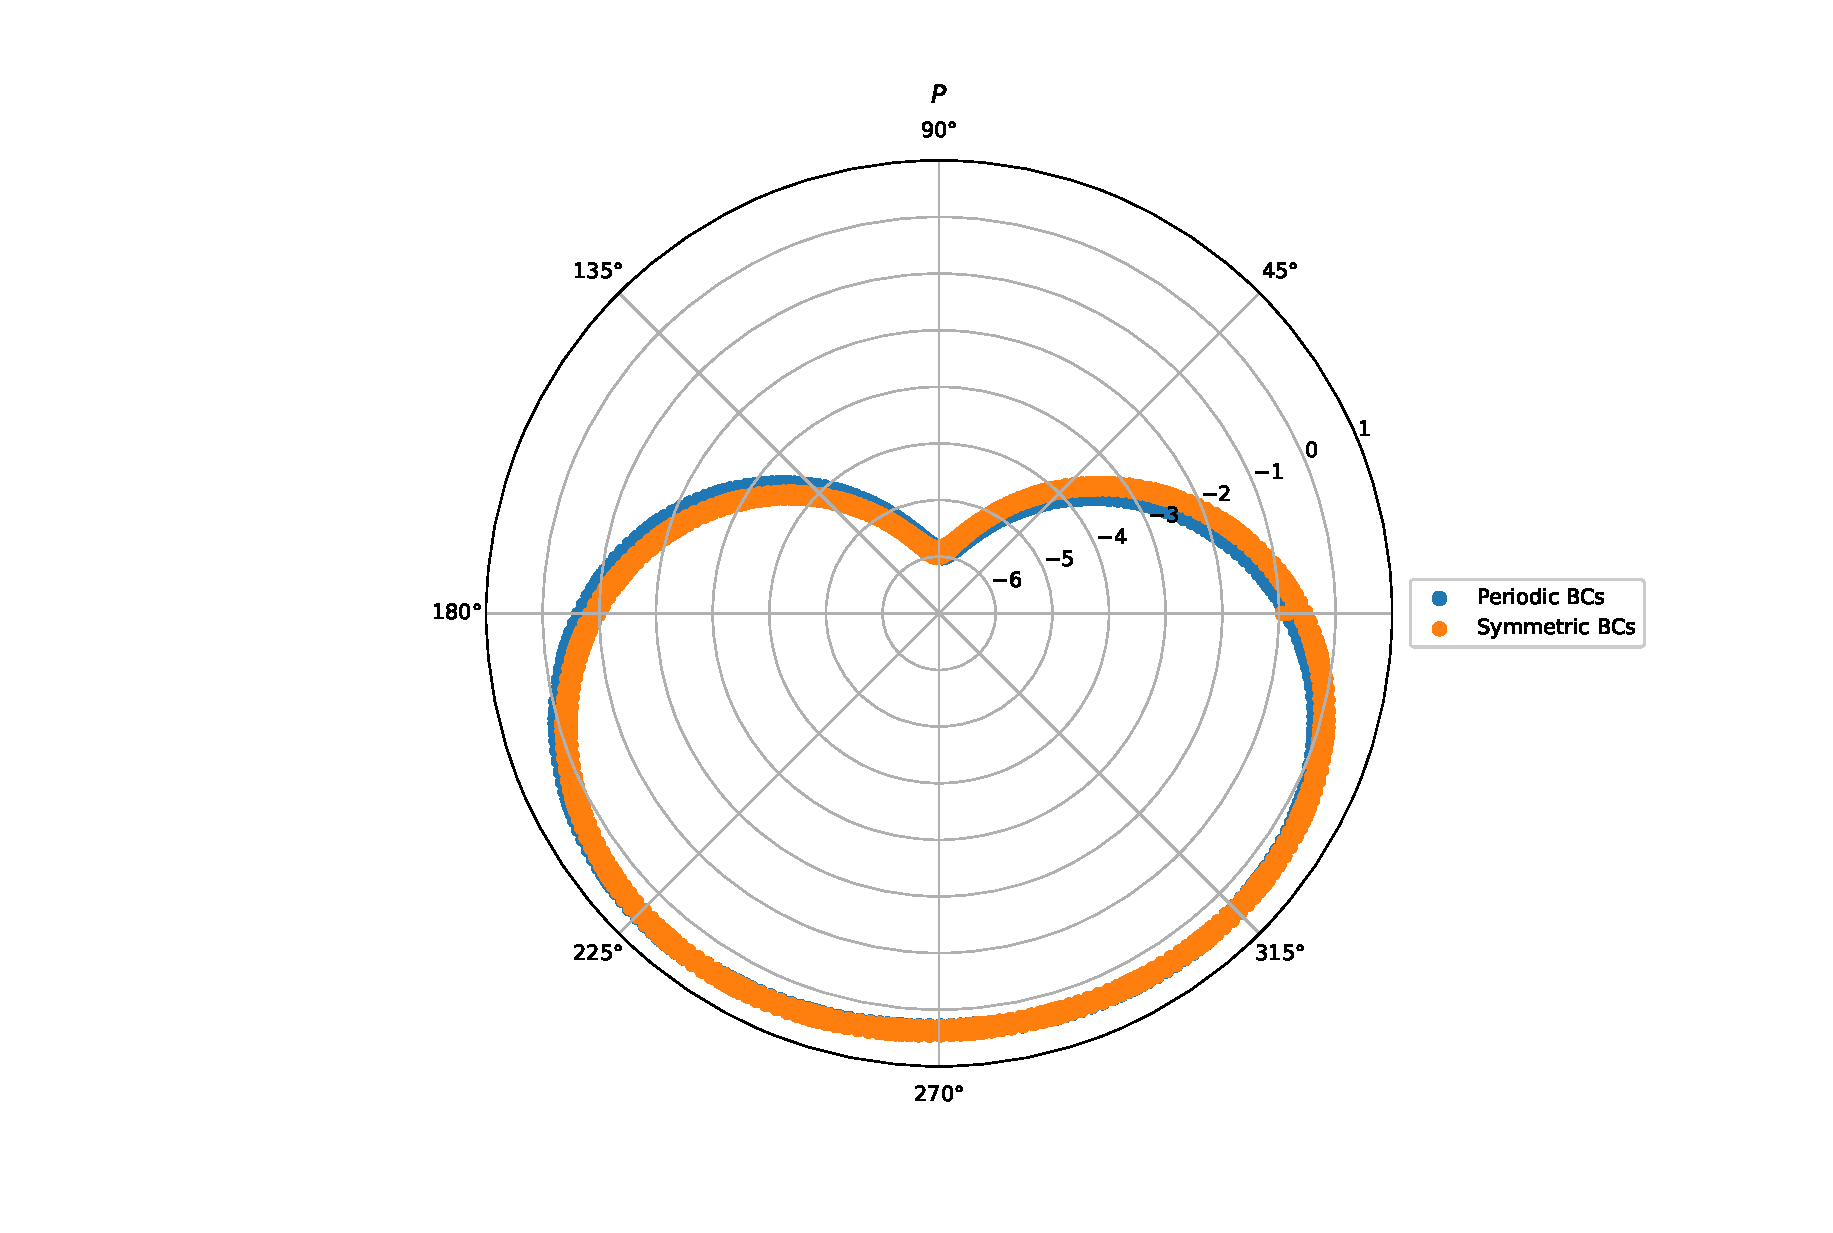
\includegraphics[width=0.9\textwidth]{polar.eps}}
    \caption{Polar plot of pressure on each surface}
    \label{fig:polar pres}
\end{figure}
The fact that the discrepancy in drag arises from the rotation of the low-pressure region explains why the drag discrepancy increases with higher rotational velocity. We now look at domains with larger heights to observe the effect of height on these discrepencies.

Figure \ref{fig:per12} shows that the rotation of the fluid is decreased as the domain height is increased. When you use periodic boundary conditions, you are in reality simulating an array (one-dimensional in this case) of cylinders. When you decrease domain heights, you increase the effect of "neighboring" cylinders on the flow. These virtual neighbors help induce more rotation in the flow. This is why there is a decrease in flow rotation with larger domain heights, which results in less negative-pressure region rotation. Less negative-pressure region rotation leads to an decrease in drag.  

In the symmetric boundary condition case, Fig. \ref{fig:sym12} shows how more rotation of the flow is allowed because the lateral boundaries are farther away from the body. This added rotation explains how the drag increases with domain size, as Fig. \ref{fig:domain_conv} shows.  
\begin{figure}
    \centering
    \begin{subfigure}{0.49\textwidth}
    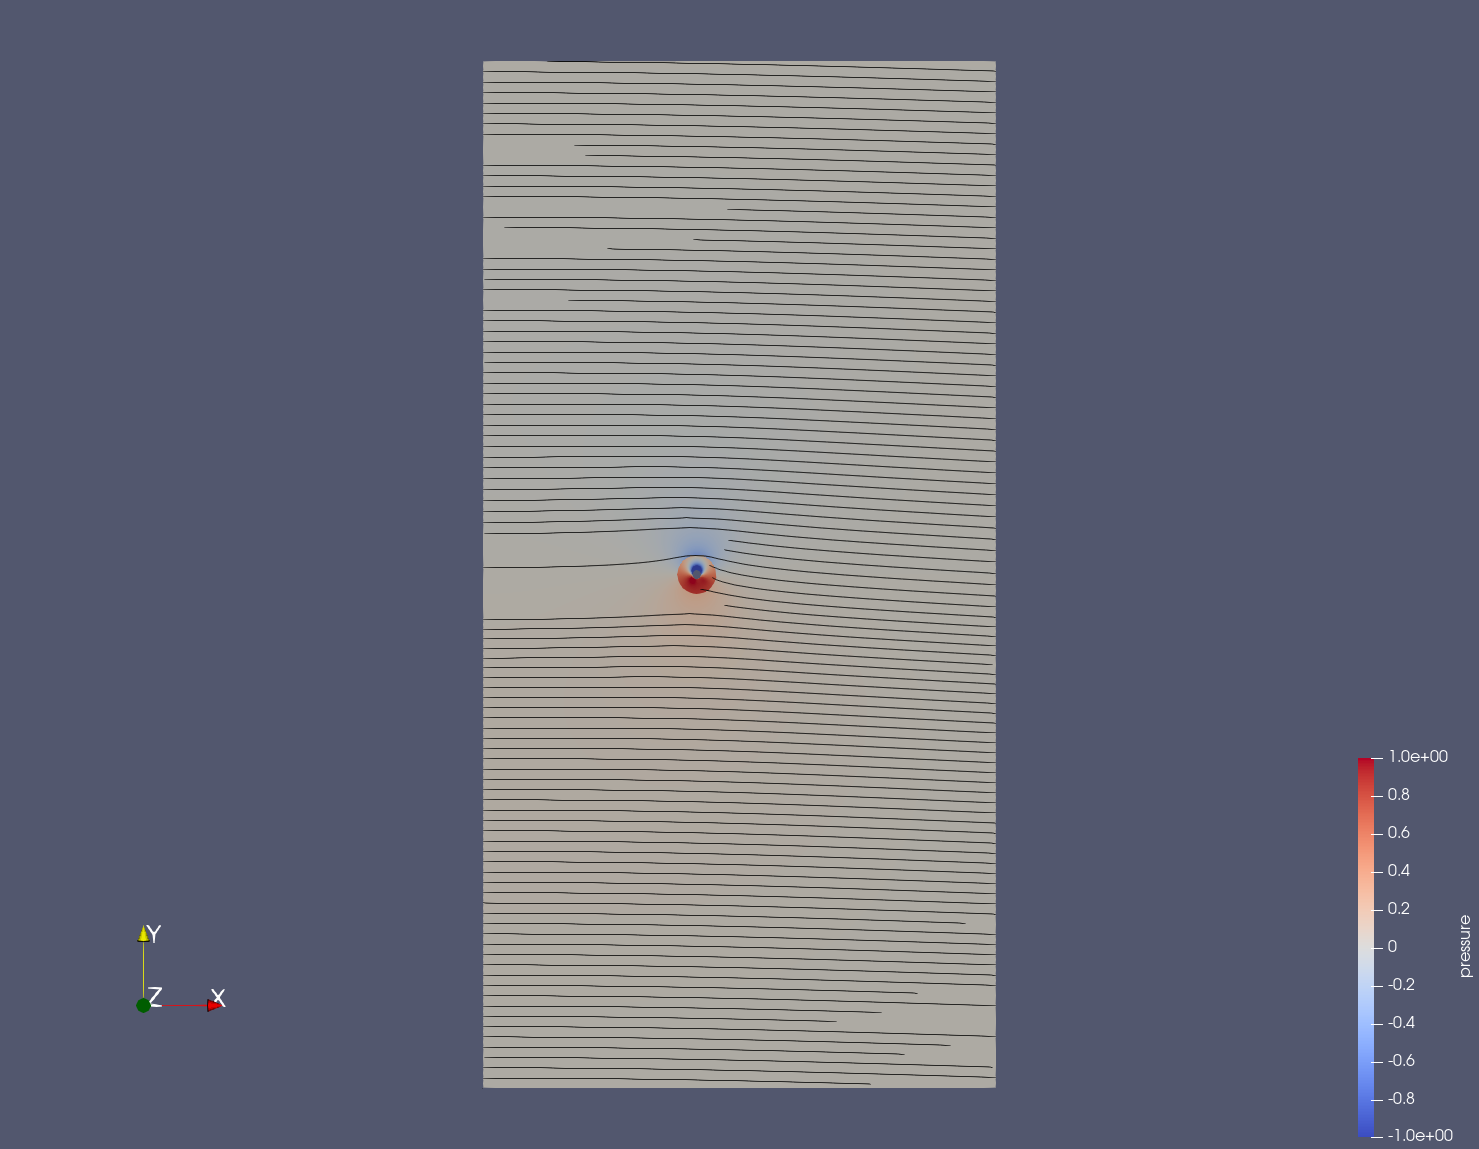
\includegraphics[width=\textwidth]{per12.png}
    \caption{Periodic boundary conditions}
    \label{fig:per12}
    \end{subfigure}
    \begin{subfigure}{0.49\textwidth}
    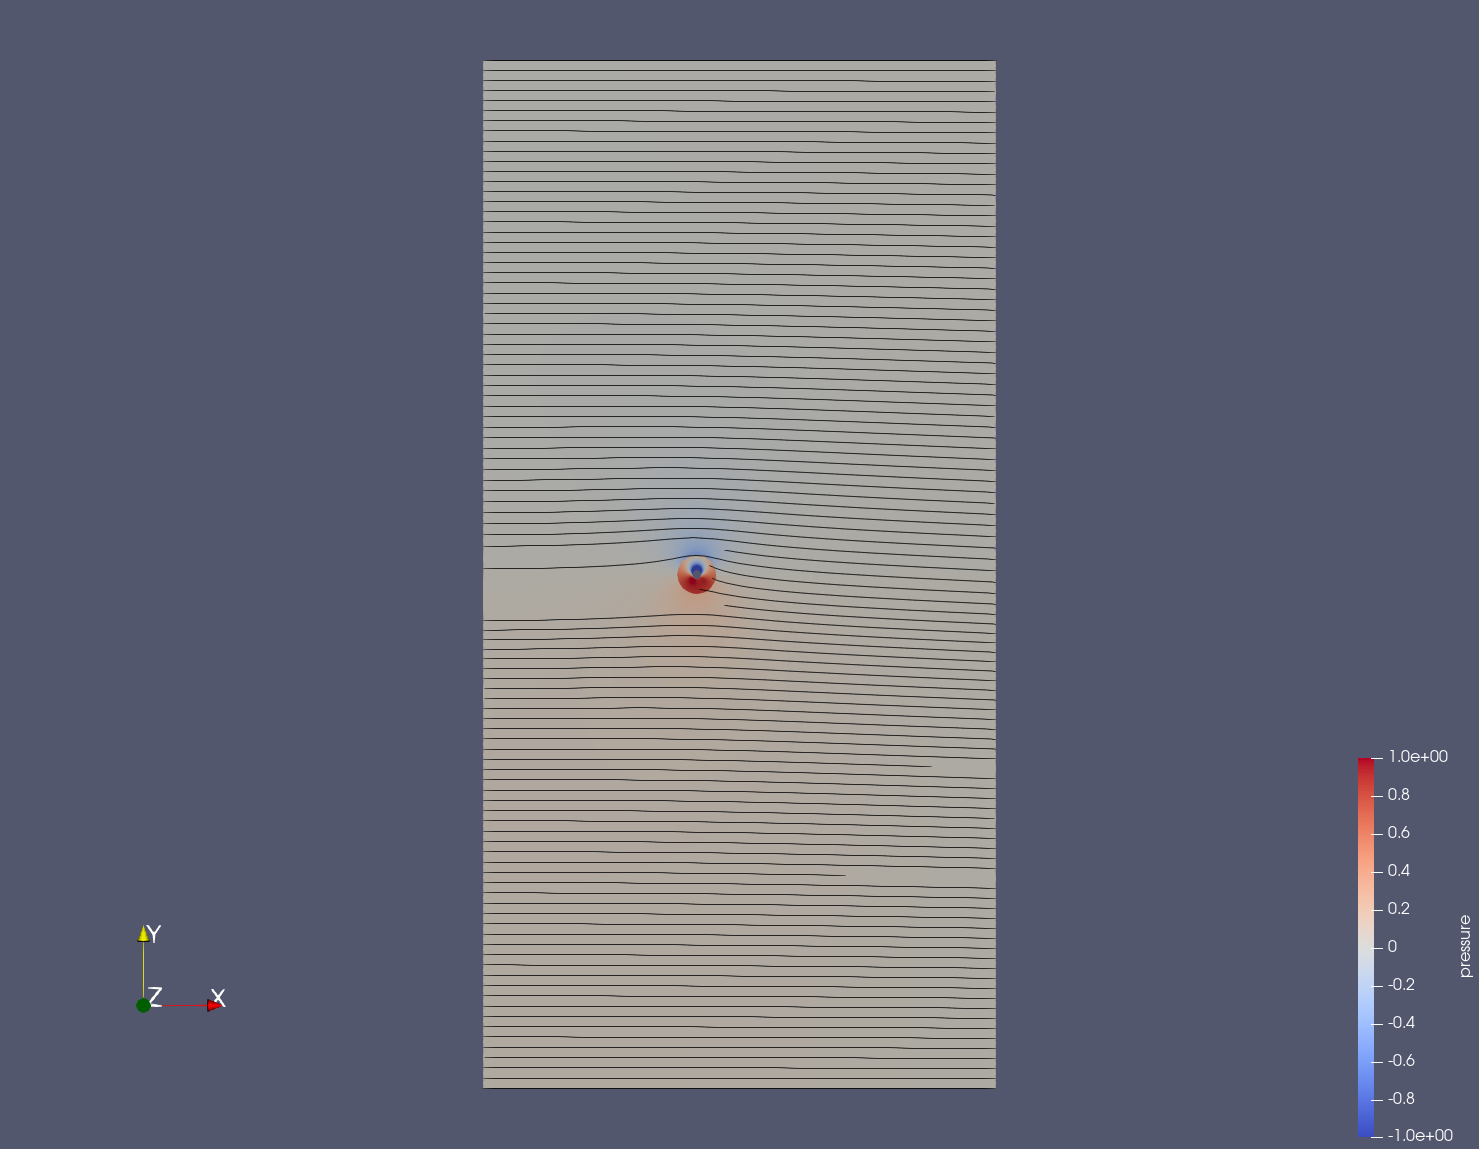
\includegraphics[width=\textwidth]{sym12.png}
    \caption{Symmetric boundary conditions}
    \label{fig:sym12}
    \end{subfigure}
    \caption{Pressure and streamline plots at $H=120D$, $\Omega^{\ast} = 3$, $\Rey = 200$, aspect ratio = 1}
    \label{fig:per sym12}
\end{figure}

Mittal and Kumar \cite{mittal_flow_2003} conducted a similar test looking only at symmetric boundary conditions. They conducted a study by varying the side length of a square mesh with a cylinder in the middle. They found that the drag values converge when the size of the domain is increased, which is consistent with our findings. However, their study changed both dimensions of the domain at the same time. Our study isolates the effect of the height of the domain. They did also find that lift is unaffected by domain size, which is consistent with our results. 

We ran our simulations with polynomial order $N = 11$. We ran a case with $N = 9, 11, 13$ which, on a grid of $E = 3712$ elements, correspond to gridpoint counts between $n = E \cdot 9^2 = 300,672$ and $n = E \cdot 13^2 = 627,328$. The change in drag is less than $1\%$ and the change in lift is less than $2\%$. The mesh independence cases were conducted on the $Fr^2 = 0.01$, $AR = 1.5$ case.

 % or Plan to meet objectives
    \chapter{Results}
\label{chp:Results}
\section{Circle results}
\label{section:Circle_results}
\subsubsection{Drag and lift}
We start by looking at time-series plots of the drag and lift of nonspinning and spinning circular cylinders as figures \ref{fig:timens} and \ref{fig:times} show. We observe that when $Fr^2$ is in the range of $[0.7, 3]$, the flow is in an unsteady, transitional flow regime. At $Fr^2 = 10$, the drag takes a while to reach a quasi-steady state. Oscillations in drag and lift occur when $Fr^2 > 1$ due to vortex-shedding. The oscillation amplitudes are larger for lift than for drag because the release of the vorticies alternates between the top and bottom of the body. The larger lift amplitudes at $Fr^2 > 10$ are explained by the fact that more stratification suppresses vortex shedding. When we have little or no stratification, the vorticies are freer to travel vertically. As expected, there is no oscillation in lift at $Fr^2 < 0.7$. The introduction of spin at $Fr^2 > 1$ increases the amplitude of the oscillation in drag. The introduction of spin also causes the lift at $Fr^2 = 10$ to take longer to converge to a quasi-steady average value. Based on these plots, we conclude that vortex-shedding transition for a spinning circle occurs somewhere in the range $Fr^2 \in (3,7)$. 

We now compare the drag and lift means between spin and no spin across different $Fr^2$ as figure \ref{fig:circleforces} shows. We observe that the addition of spin affects the average lift but not the average drag, and there is no lift when spin is absent. These two observations are consistent with the Kutta-Joukouski Theorem. The effects of stratification particularly manifest themselves when $Fr^2 < 1$. The substantial increase in drag with increase in stratification due to upstream \textit{blocking}, or \textit{vertical confinement} is a well-known phenomenon also observed by \cite{deng_drag_2022} and \cite{ortiz-tarin_stratified_2019}. These plots show that differences in the flow between $Fr^2 = 100$ and homogeneous flow is negligible. This suggests that flows at $Fr^2 = 100$ can be approximated as homogeneous. We look at the comparison of static and spinning pressure plots for circular bodies that figure \ref{fig:circle_pressure} shows. The pressure distributions change marginally as $Fr^2$ decreases up till $Fr^2 = 0.1$. At this point, a transition occurs in the pressure distribution. The isobaric regions become flattened as a result of stratification limiting vertical fluid interaction by means of a potential energy barrier. This leads to a buildup of pressure in front of the body. This effect increases when $Fr^2 = 0.01$. 

As stratification increases, there is an overall negative trend in lift. The key difference between the spin and no spin cases is the presence of a strong negative pressure field above the spinning bodies. This negative pressure zone is the main phenomenon behind the lift seen in earlier plots and is a result of the Magnus Effect. This relative low pressure zone goes away when $Fr^2 < 1$ as stratification increases. 
\begin{figure}
    \centerline{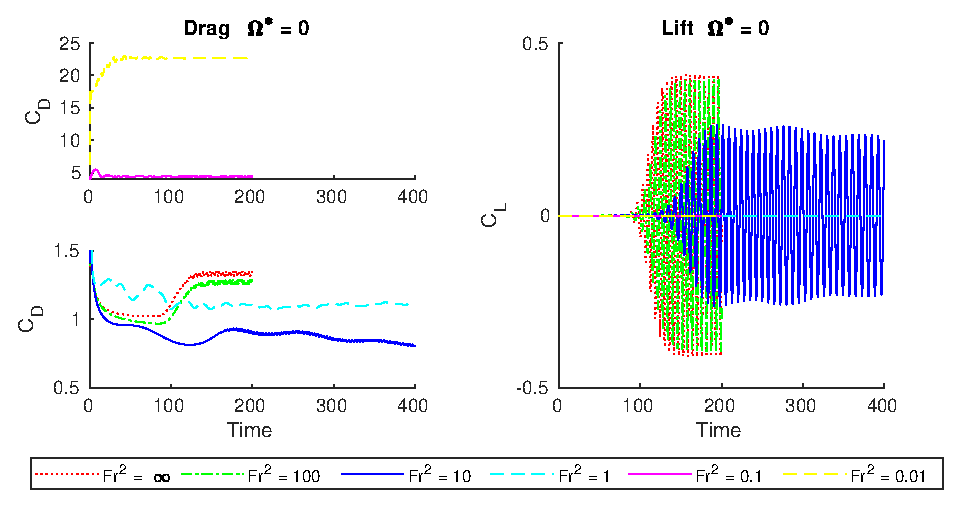
\includegraphics[width=\textwidth]{images/circle/timens.eps}}
    \caption{Time series data for nonspinning circle}
    \label{fig:timens}
\end{figure}
\begin{figure}
    \centerline{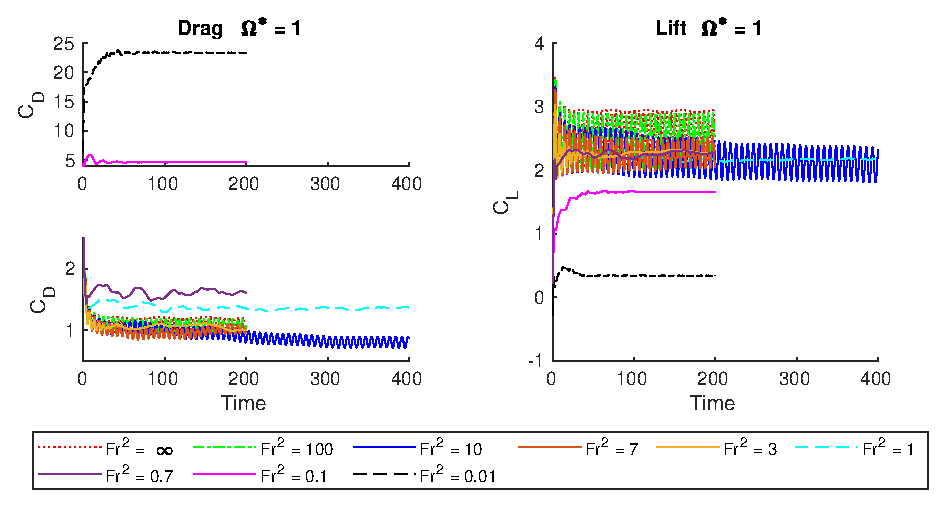
\includegraphics[width=\textwidth]{images/circle/times.eps}}
    \caption{Time series data for spinning circle}
    \label{fig:times}
\end{figure}

\begin{figure}
    \centering
    \begin{subfigure}[b]{0.49\textwidth}
        \centering
        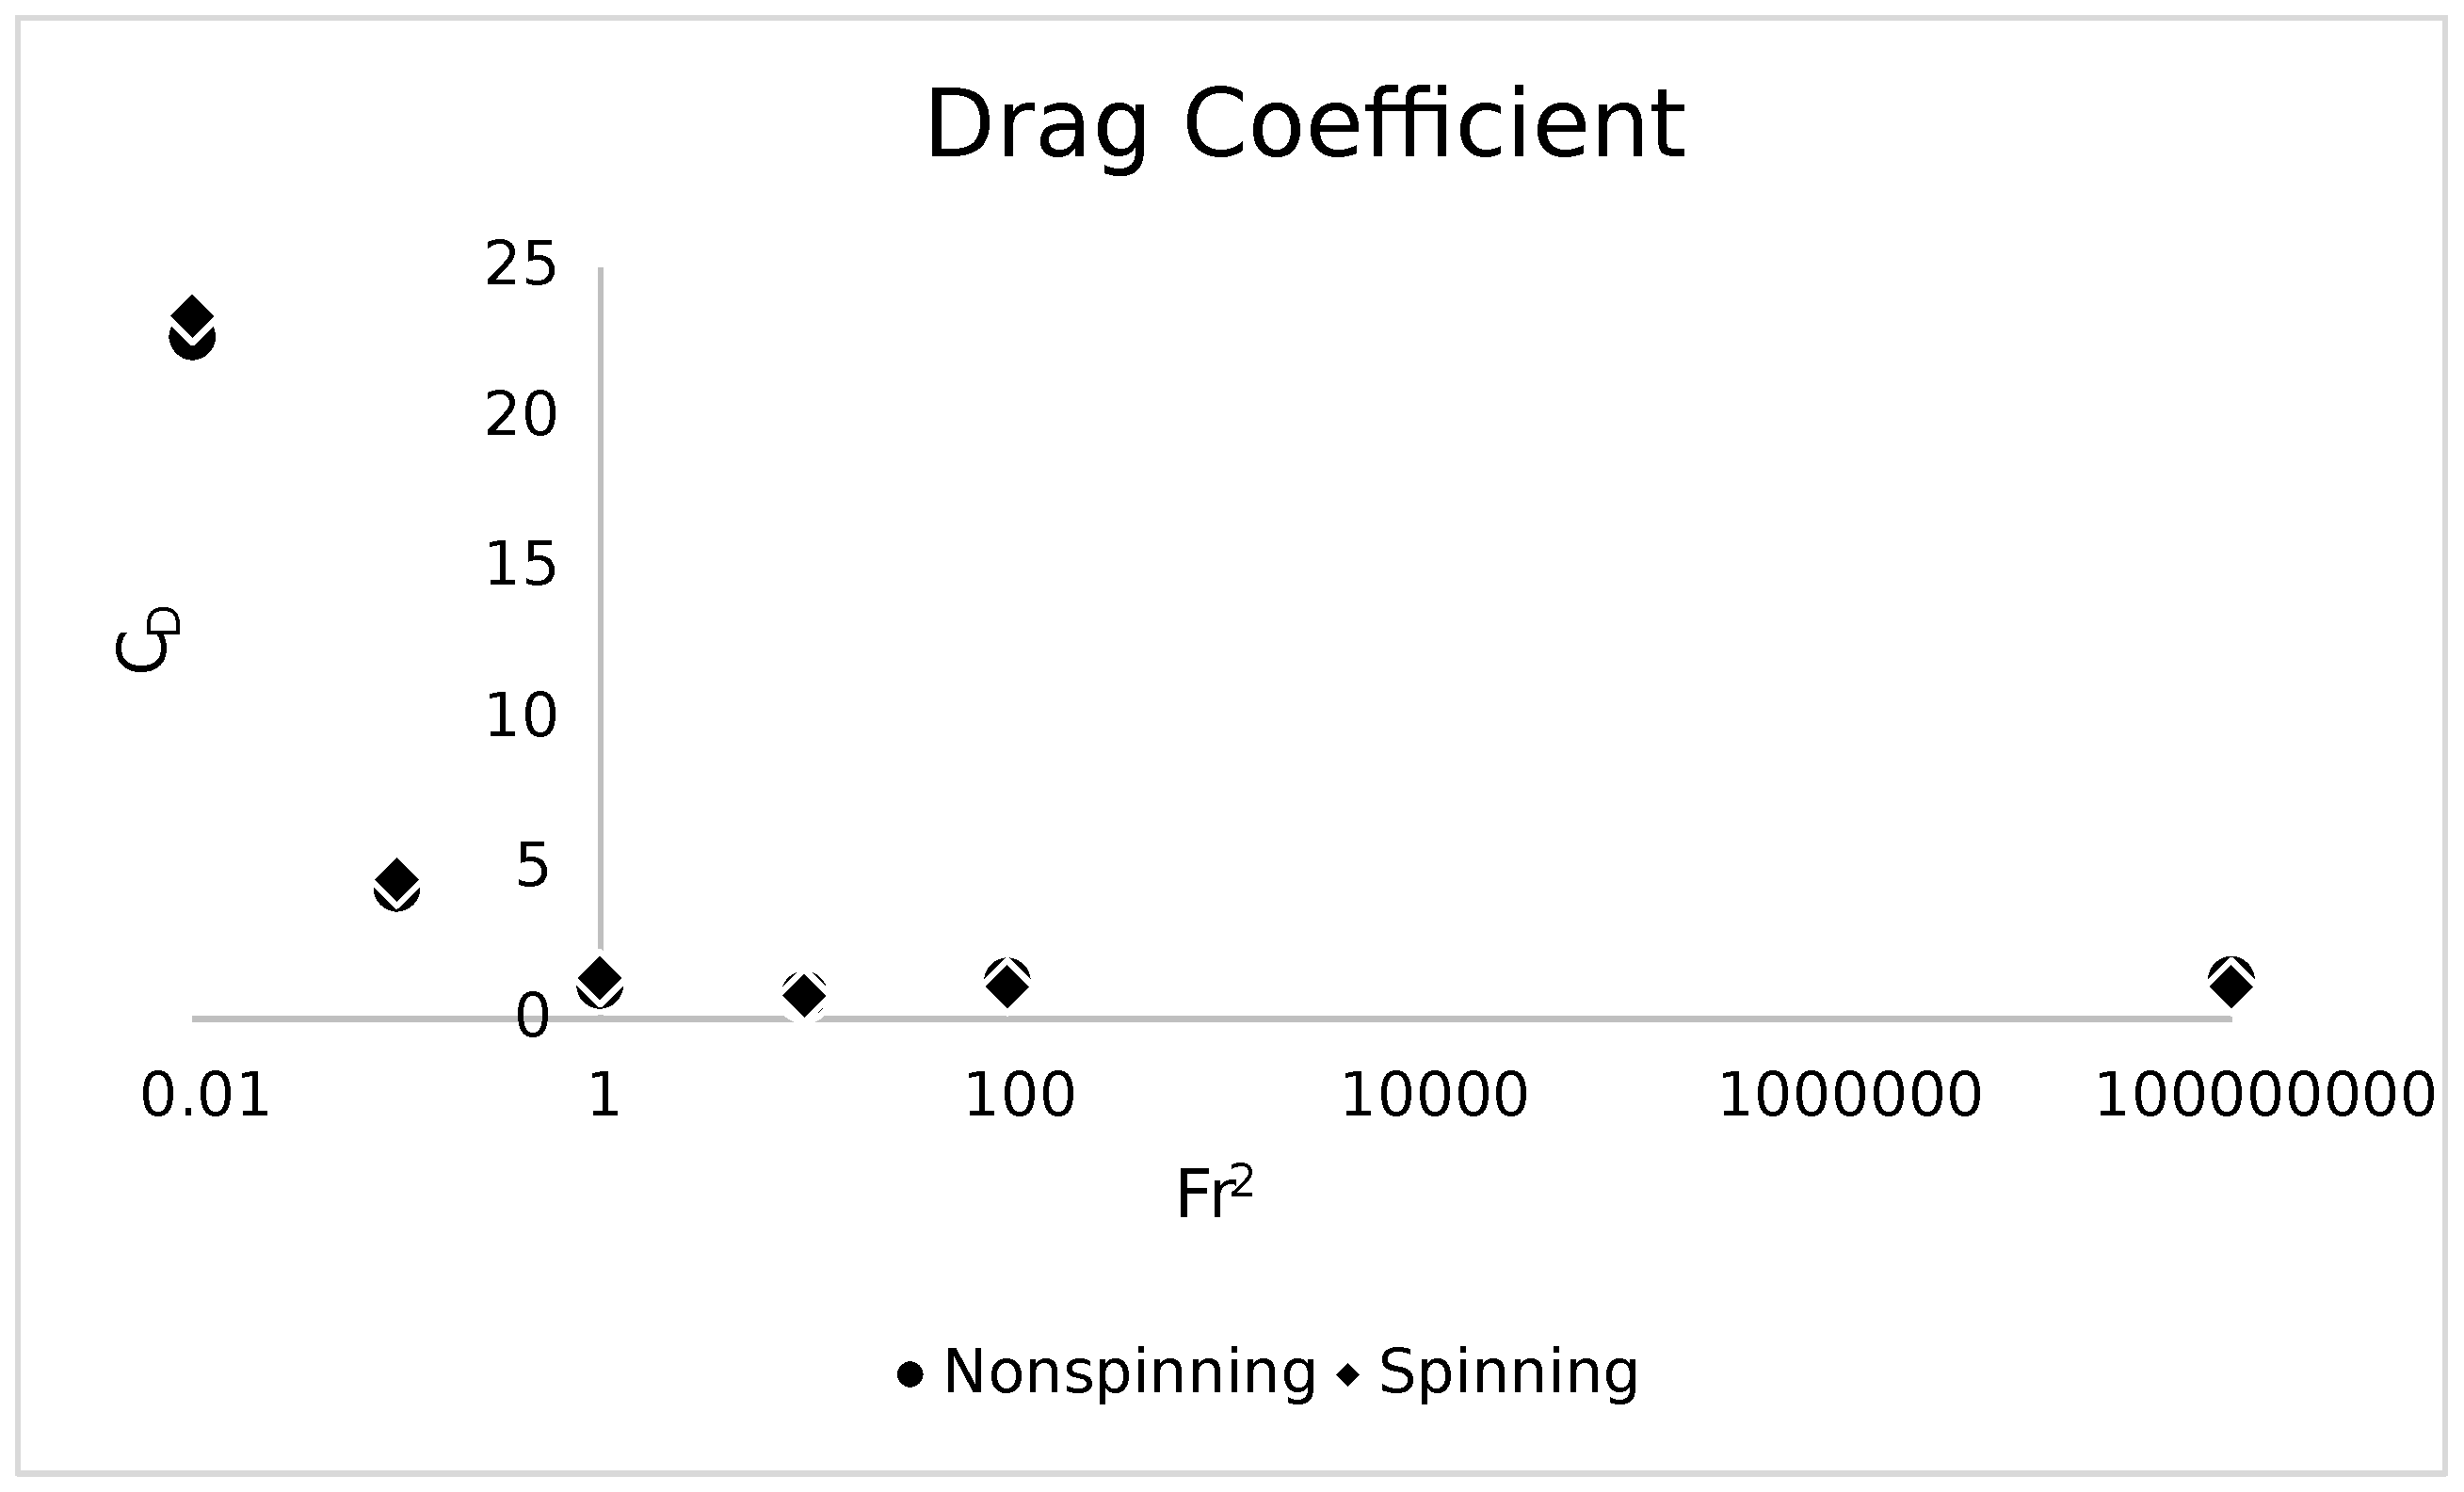
\includegraphics[width=\textwidth]{images/circle/ar1drag.eps}
        \caption{Drag coefficients}
        \label{fig:ar1drag}
    \end{subfigure}
    \hfill
    \begin{subfigure}[b]{0.49\textwidth}
        \centering
        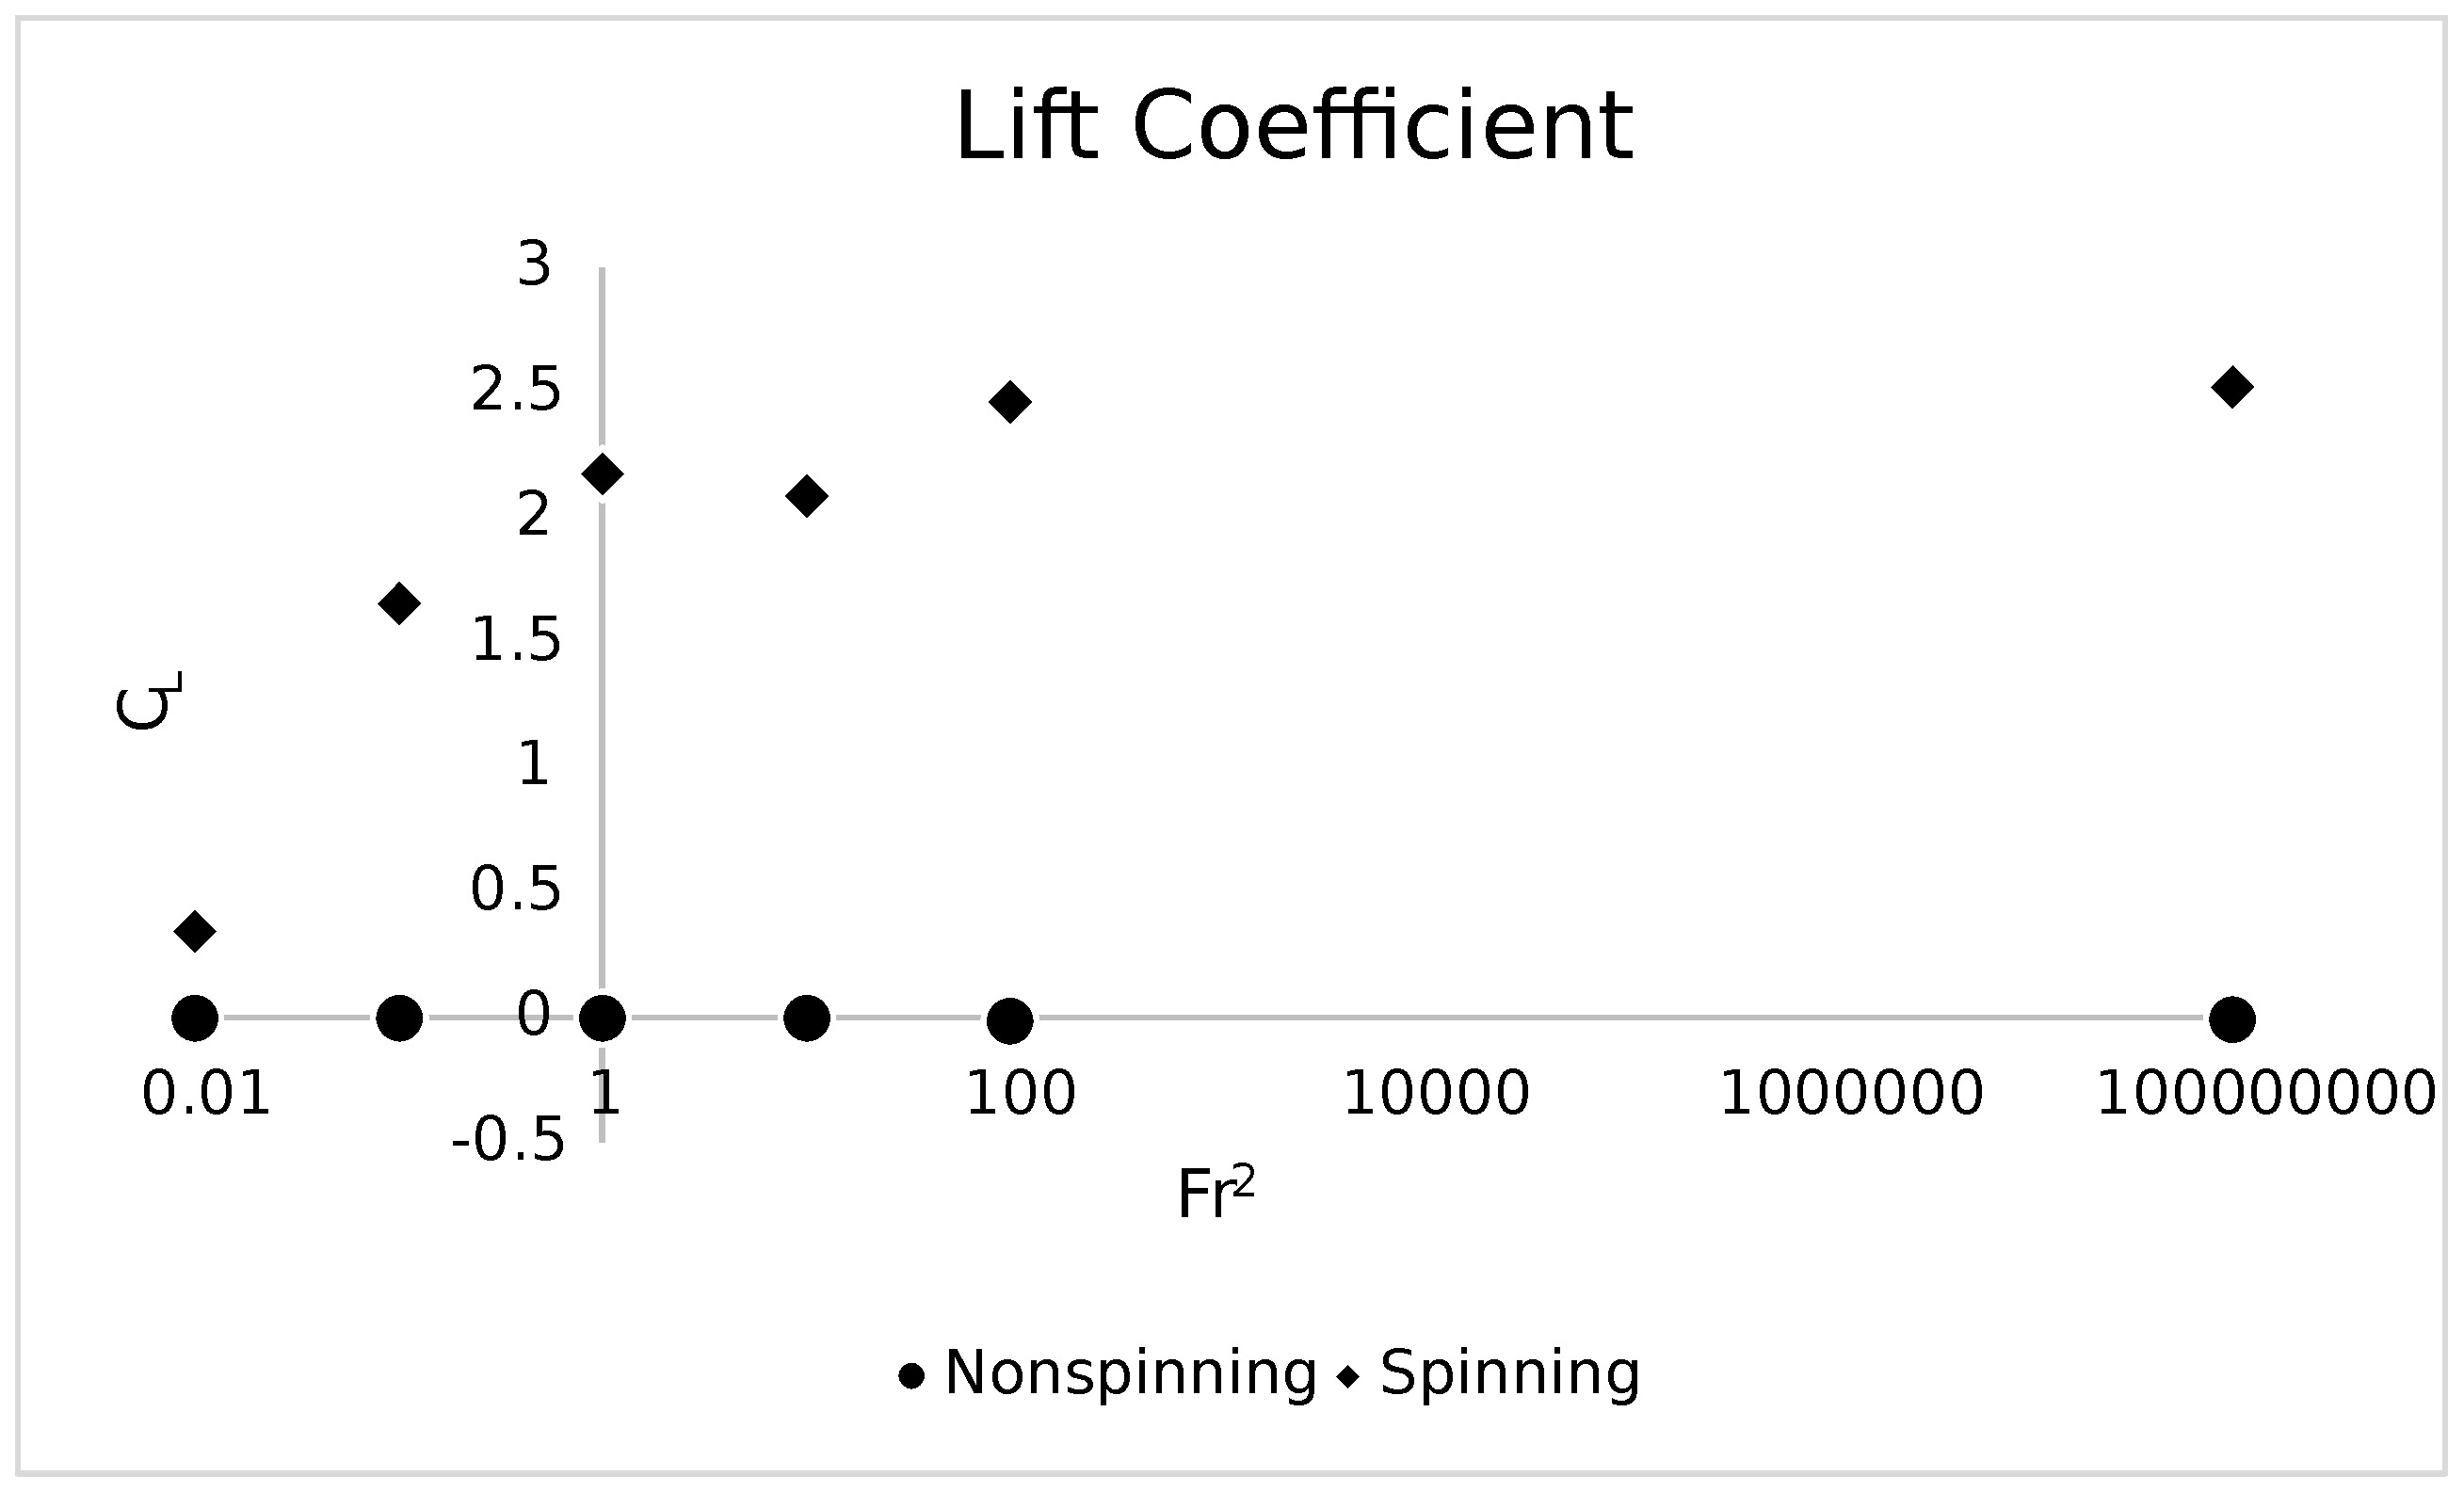
\includegraphics[width=\textwidth]{images/circle/ar1lift.eps}
        \caption{Lift coefficients}
        \label{fig:ar1lift}
    \end{subfigure}
    \caption{Mean drag and lift values for $\Omega^{\ast} = {0,1}$}
    \label{fig:circleforces}
\end{figure} 
\begin{figure}   
    \centering
        \begin{subfigure}[b]{0.25\textwidth}
        \centering
        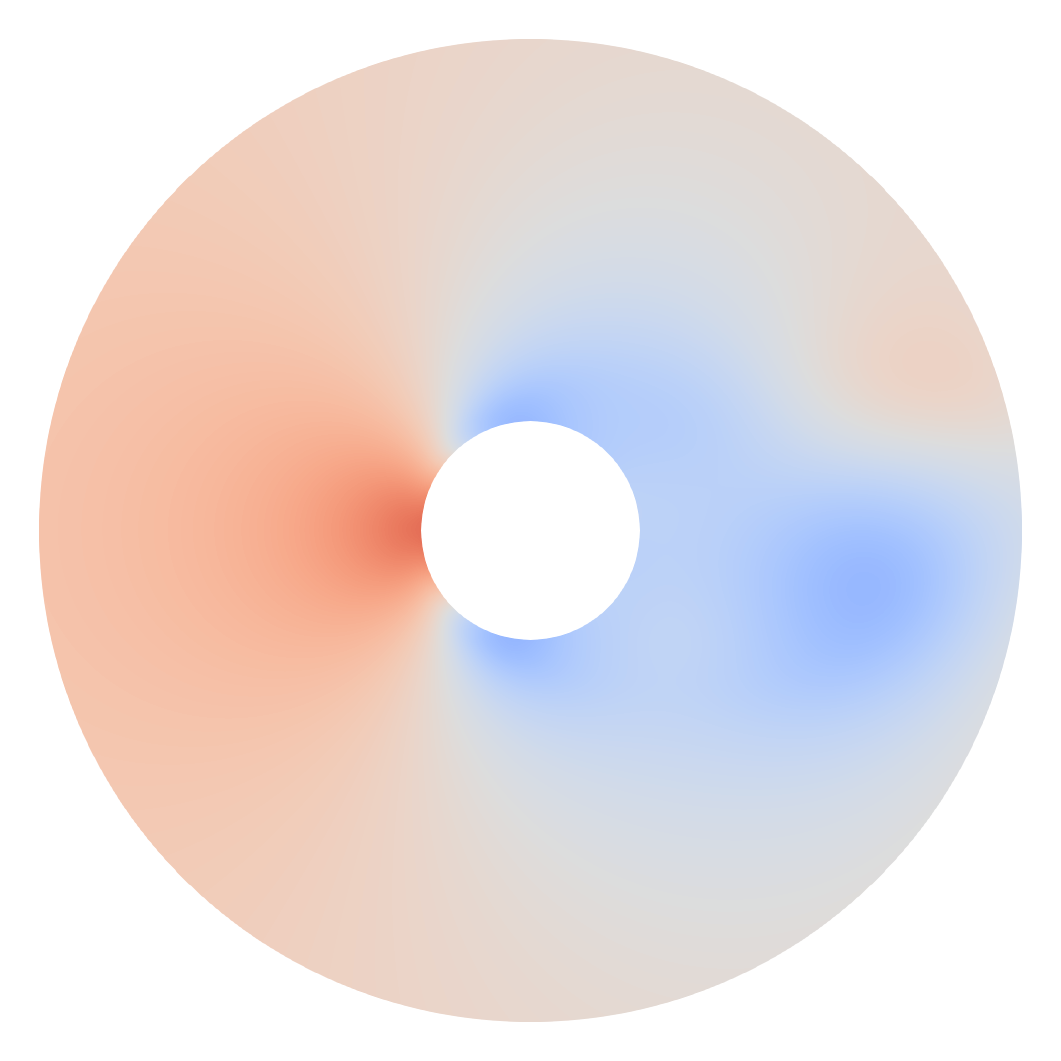
\includegraphics[width=\textwidth]{images/circle/ps0fsinf.png}
        \caption{$Fr^2 = \infty, \Omega^{\ast} = 0$}
        \label{fig:ps0fsinf}
    \end{subfigure}
    \hfill
    \begin{subfigure}[b]{0.25\textwidth}
        \centering
        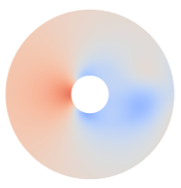
\includegraphics[width=\textwidth]{images/circle/ps0fs100.png}
        \caption{$Fr^2 = 100, \Omega^{\ast} = 0$}
        \label{fig:ps0fs100}
    \end{subfigure}
    \hfill
    \begin{subfigure}[b]{0.25\textwidth}
        \centering
        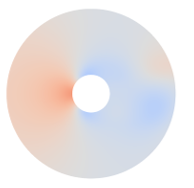
\includegraphics[width=\textwidth]{images/circle/ps0fs10.png}
        \caption{$Fr^2 = 10, \Omega^{\ast} = 0$}
        \label{fig:ps0fs10}
    \end{subfigure}
    
    \begin{subfigure}[b]{0.25\textwidth}
        \centering
        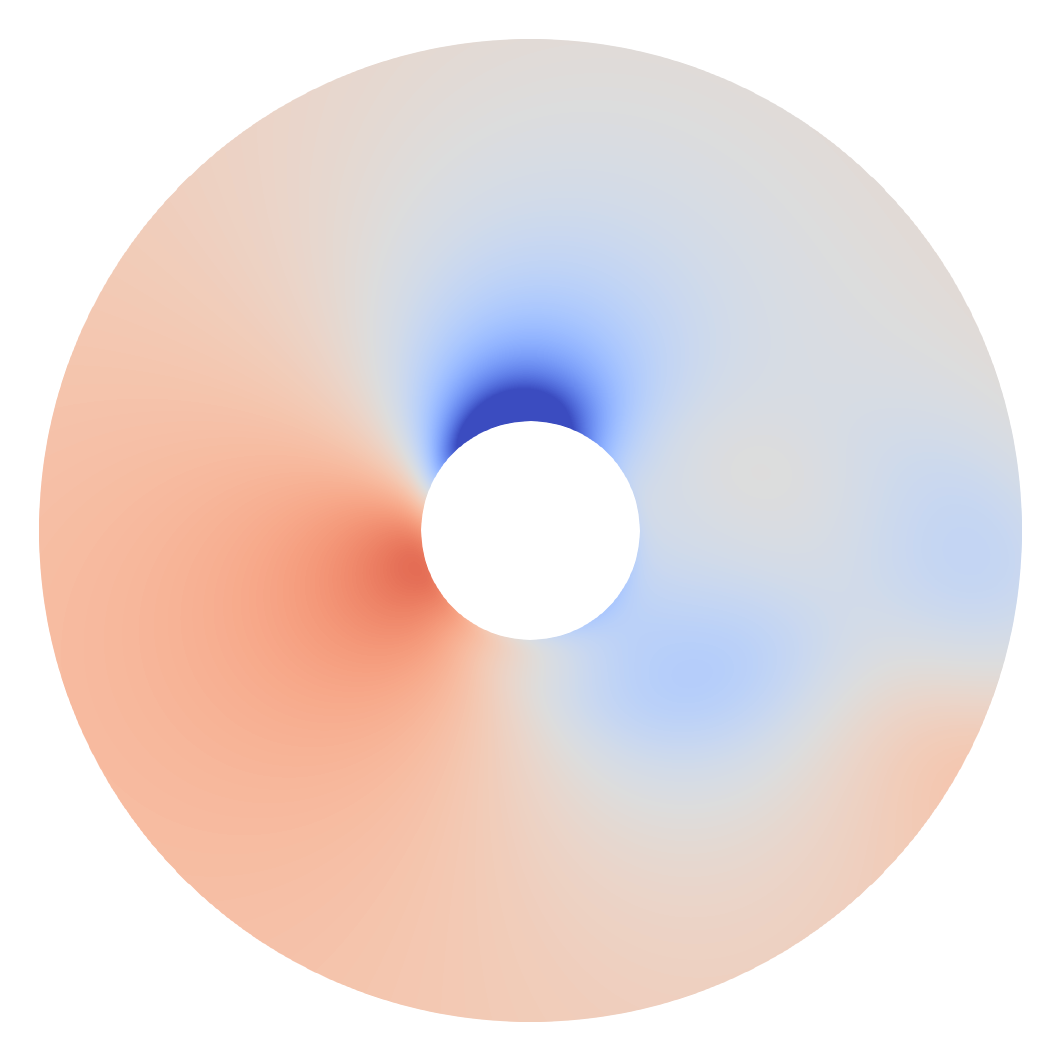
\includegraphics[width=\textwidth]{images/circle/ps1fsinf.png}
        \caption{$Fr^2 = \infty, \Omega^{\ast} = 1$}
        \label{fig:ps1fsinf}
    \end{subfigure}
    \hfill
    \begin{subfigure}[b]{0.25\textwidth}
        \centering
        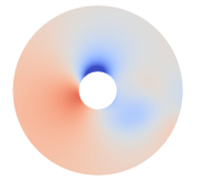
\includegraphics[width=\textwidth]{images/circle/ps1fs100.png}
        \caption{$Fr^2 = 100, \Omega^{\ast} = 1$}
        \label{ps1fs100}
    \end{subfigure}
    \hfill
    \begin{subfigure}[b]{0.25\textwidth}
        \centering
        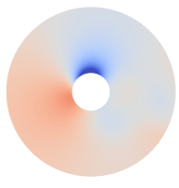
\includegraphics[width=\textwidth]{images/circle/ps1fs10.png}
        \caption{$Fr^2 = 10, \Omega^{\ast} = 1$}
        \label{fig:ps1fs10}
    \end{subfigure}

    \begin{subfigure}[b]{0.25\textwidth}
        \centering
        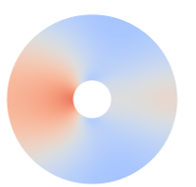
\includegraphics[width=\textwidth]{images/circle/ps0fs1.png}
        \caption{$Fr^2 = 1, \Omega^{\ast} = 0$}
        \label{fig:ps0fs1}
    \end{subfigure}
    \hfill
    \begin{subfigure}[b]{0.25\textwidth}
        \centering
        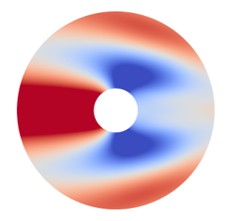
\includegraphics[width=\textwidth]{images/circle/ps0fs0p1.png}
        \caption{$Fr^2 = 0.1, \Omega^{\ast} = 0$}
        \label{fig:ps0fs0p1}
    \end{subfigure}
    \hfill
    \begin{subfigure}[b]{0.25\textwidth}
        \centering
        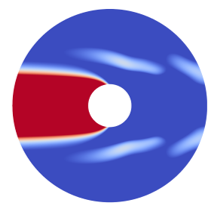
\includegraphics[width=\textwidth]{images/circle/ps0fs0p01.png}
        \caption{$Fr^2 = 0.01, \Omega^{\ast} = 0$}
        \label{fig:ps0fs0p01}
    \end{subfigure}

    \begin{subfigure}[b]{0.25\textwidth}
        \centering
        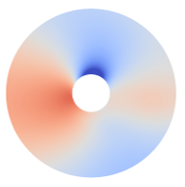
\includegraphics[width=\textwidth]{images/circle/ps1fs1.png}
        \caption{$Fr^2 = 1, \Omega^{\ast} = 1$}
        \label{fig:ps1fs1}
    \end{subfigure}
    \hfill
    \begin{subfigure}[b]{0.25\textwidth}
        \centering
        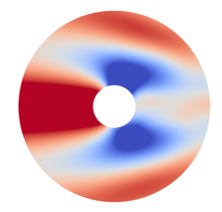
\includegraphics[width=\textwidth]{images/circle/ps1fs0p1.png}
        \caption{$Fr^2 = 0.1, \Omega^{\ast} = 1$}
        \label{fig:ps1fs0p1}
    \end{subfigure}
    \hfill
    \begin{subfigure}[b]{0.25\textwidth}
        \centering
        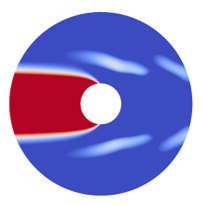
\includegraphics[width=\textwidth]{images/circle/ps1fs0p01.png}
        \caption{$Fr^2 = 0.01, \Omega^{\ast} = 1$}
        \label{fig:ps1fs0p01}
    \end{subfigure}
    
    \begin{subfigure}[b]{0.25\textwidth}
        \centering
        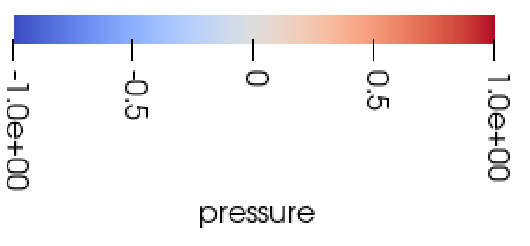
\includegraphics[width=\textwidth]{images/circle/p_scale.png}
        \caption*{}
    \end{subfigure}
    
    \caption{A comparison of the pressure fields for nonspinning and spinning circles}
    \label{fig:circle_pressure}
\end{figure}
\clearpage
\subsubsection{Flow structures}
We look at the y-velocity plot that figure \ref{fig:circle y-vel} shows. We observe that introducing spin does not significantly alter the flow at $Fr^2 < 1$. At $Fr^2 > 1$, the eddy wake is rotated clockwise, as expected. The plots show that the flow regime in both cases at $Fr^2 = 1$ is in transition. The vortex shedding that exists with lower stratification diminishes at $Fr^2 = 1$ as stratification increases. The plots show that there is an optimal level of stratification for gravity propagation. The plots show that at the edges of our $Fr^2$ parameter space, the gravity waves do not propagate well. The gravity waves propagate best at around $Fr^2 = 1$. We observe periodic semi-circular patterns at $Fr^2 = 1, 0.1$ that is also observed by \cite{ortiz-tarin_stratified_2019}.\\ 
We include schlerien plots (first derivative in density) in figure \ref{fig:circleschlerien}. The schlerien plots better capture the flow structures at higher $Fr^2$; the y-velocity plots do not fully capture the details of the vortex-shedding that occurs at high $Fr^2$. At $Fr^2 = 7, 10$, the schlerien plots show competition between a vortex-dominated-regime and an internal-gravity-wave-regime. At these $Fr^2$ numbers, we see the formation of vortices and their breakdown, while in the internal-gravity-wave-regime where $Fr^2 < 7$ there is no vortex-shedding. 
The reason the strength of the propagation of gravity waves is not linear is because there are two competing phenomena. The first phenomenon is the requirement of a restoring force for oscillation. This restoring forces comes from the density gradient, and the larger the density gradient, the larger the restoring force. The other phenomenon is the resistance of vertical motion due to stratification. This resistance increases with stratification. The combination of these competing phenomena result in an optimum level of stratification for gravity wave propagation. We observe that at low $Fr^2$, the IGW have little amplitude but do not dissipate easily. The reason for this high potential from high stratification is very sensitive to displacements. The IGW will still have small amplitudes, but the vertical high information-dependence across the domain will allow little dissipation. In the case of $Fr^2 = 0.01$, the dissipation is so weak that the IGW are spuriously reflecting off the boundaries.  
We see that the two phenomena are competing at $Fr^2 = 10$. Vortex-shedding is occurring, but is being suppressed. Gravity waves are present, but weak. This explains why in our time-series and ensemble-average plots the drag values do not settle to a steady value.
The flow pattern we observe in the cases of $Fr^2 \in [7, 10]$ in which a wake whose scale is on the order of the cylinder breaks down into smaller-scale wakes. This feature is also observed by \cite{deng_drag_2022} for a nonspinning circle, who states this feature does not exist in homogeneous flows. This feature does not exist in unstratified flows because there is no potential energy barrier resisting vertical motion like there is in stratified flow. In stratified flows, the resistance to vertical motion causes the wakes and vorticies to break down into features with less vertical displacement. An observation that confirms the earlier mathematically extracted hypothesis from equation \ref{eq:nondim NBV} that as we increase our stratification, our Brunt–Väisälä frequency increases. This phenomenon manifests itself in the decrease in the wavelength of the gravity waves in the plots.


\begin{figure}   
    \centering
        \begin{subfigure}[b]{0.32\textwidth}
        \centering
        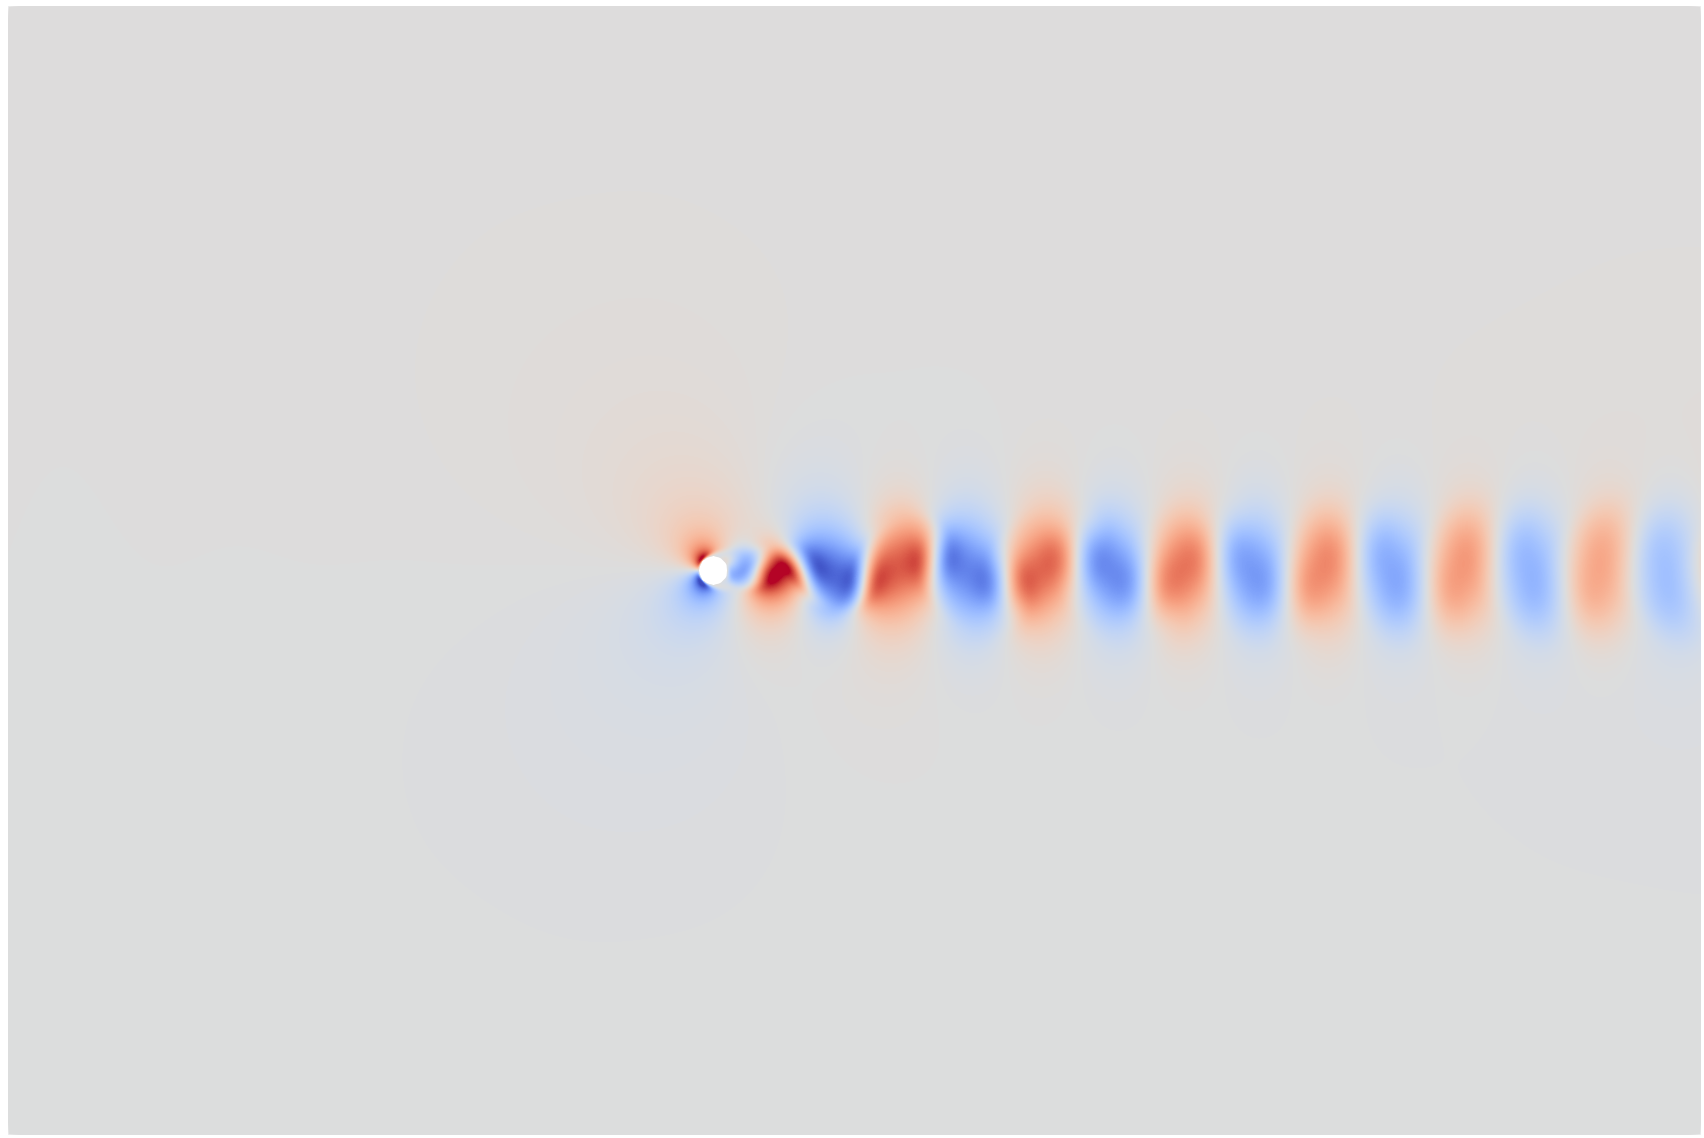
\includegraphics[width=\textwidth]{images/circle/av0fsinf.png}
        \caption{$Fr^2 = \infty, \Omega^{\ast} = 0$}
        \label{fig:av0fsinf}
    \end{subfigure}
    \hfill
    \begin{subfigure}[b]{0.32\textwidth}
        \centering
        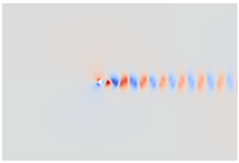
\includegraphics[width=\textwidth]{images/circle/av0fr10.png}
        \caption{$Fr^2 = 100, \Omega^{\ast} = 0$}
        \label{fig:av0frs100}
    \end{subfigure}
    \hfill
    \begin{subfigure}[b]{0.32\textwidth}
        \centering
        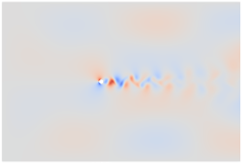
\includegraphics[width=\textwidth]{images/circle/av0fr3.png}
        \caption{$Fr^2 = 10, \Omega^{\ast} = 0$}
        \label{fig:av0frs10}
    \end{subfigure}
    
    \begin{subfigure}[b]{0.32\textwidth}
        \centering
        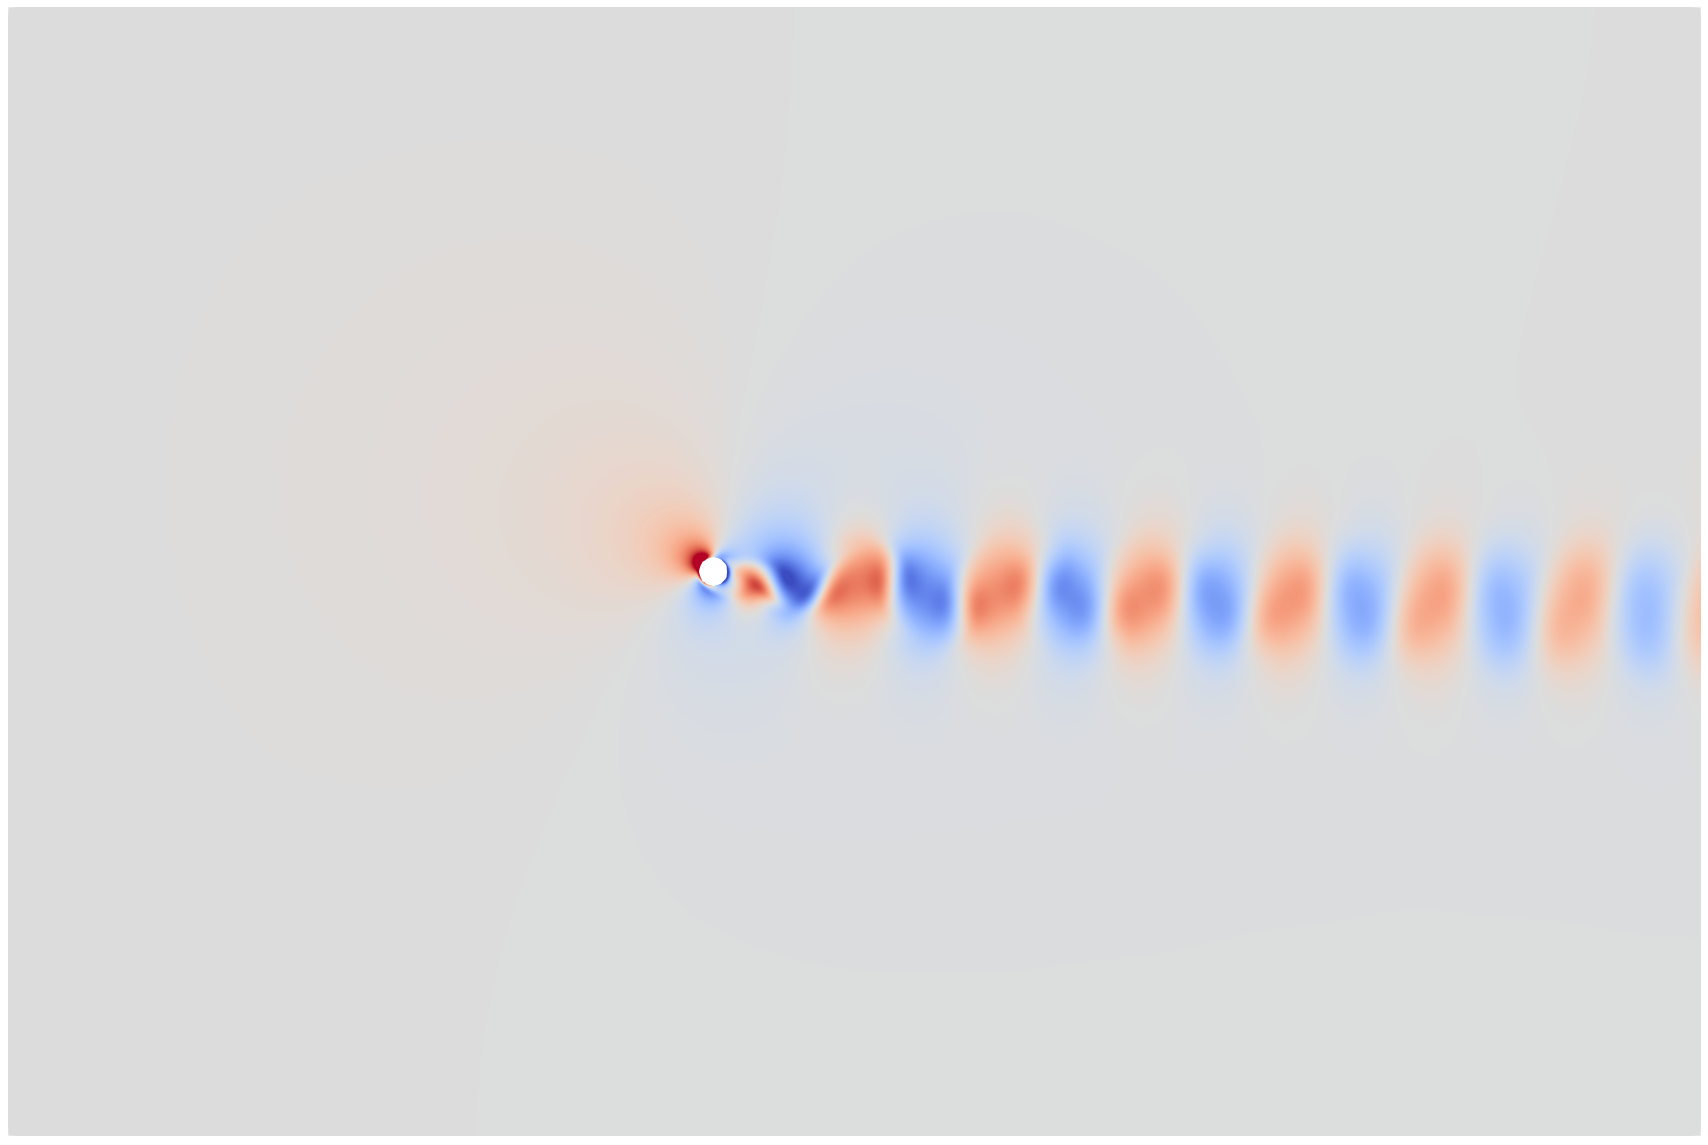
\includegraphics[width=\textwidth]{images/circle/av1fsinf.png}
        \caption{$Fr^2 = \infty, \Omega^{\ast} = 1$}
        \label{fig:av1fsinf}
    \end{subfigure}
    \hfill
    \begin{subfigure}[b]{0.32\textwidth}
        \centering
        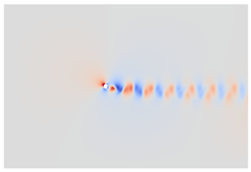
\includegraphics[width=\textwidth]{images/circle/av1fr10.png}
        \caption{$Fr^2 = 100, \Omega^{\ast} = 1$}
        \label{av1frs100}
    \end{subfigure}
    \hfill
    \begin{subfigure}[b]{0.32\textwidth}
        \centering
        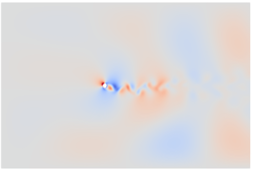
\includegraphics[width=\textwidth]{images/circle/av1fr3.png}
        \caption{$Fr^2 = 10, \Omega^{\ast} = 1$}
        \label{fig:av1frs10}
    \end{subfigure}

    \begin{subfigure}[b]{0.32\textwidth}
        \centering
        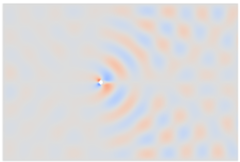
\includegraphics[width=\textwidth]{images/circle/av0fr1.png}
        \caption{$Fr^2 = 1, \Omega^{\ast} = 0$}
        \label{fig:av0frs1}
    \end{subfigure}
    \hfill
    \begin{subfigure}[b]{0.32\textwidth}
        \centering
        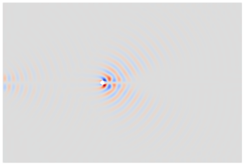
\includegraphics[width=\textwidth]{images/circle/av0fr0p3.png}
        \caption{$Fr^2 = 0.1, \Omega^{\ast} = 0$}
        \label{fig:av0frs0p1}
    \end{subfigure}
    \hfill
    \begin{subfigure}[b]{0.32\textwidth}
        \centering
        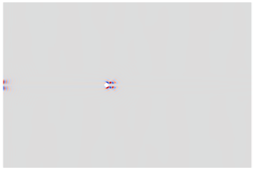
\includegraphics[width=\textwidth]{images/circle/av0fr0p1.png}
        \caption{$Fr^2 = 0.01, \Omega^{\ast} = 0$}
        \label{fig:av0frs0p01}
    \end{subfigure}

    \begin{subfigure}[b]{0.32\textwidth}
        \centering
        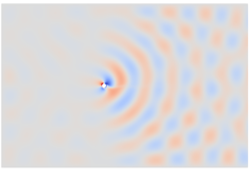
\includegraphics[width=\textwidth]{images/circle/av1fr1.png}
        \caption{$Fr^2 = 1, \Omega^{\ast} = 1$}
        \label{fig:av1frs1}
    \end{subfigure}
    \hfill
    \begin{subfigure}[b]{0.32\textwidth}
        \centering
        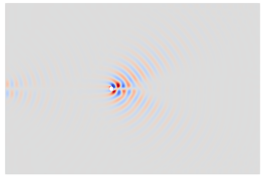
\includegraphics[width=\textwidth]{images/circle/av1fr0p3.png}
        \caption{$Fr^2 = 0.1, \Omega^{\ast} = 1$}
        \label{fig:av1frs0p1}
    \end{subfigure}
    \hfill
    \begin{subfigure}[b]{0.32\textwidth}
        \centering
        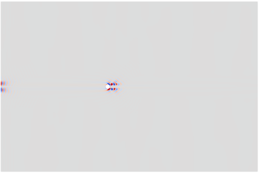
\includegraphics[width=\textwidth]{images/circle/av1fr0p1.png}
        \caption{$Fr^2 = 0.01, \Omega^{\ast} = 1$}
        \label{fig:av1frs0p01}
    \end{subfigure}
    
    \begin{subfigure}[b]{0.32\textwidth}
        \centering
        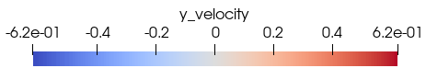
\includegraphics[width=\textwidth]{images/circle/scale.png}
        \caption*{}
    \end{subfigure}
    
    \caption{A comparison of the y-velocity fields for nonspinning and spinning circles}
    \label{fig:circle y-vel}
\end{figure}

\begin{figure}
    \centering
    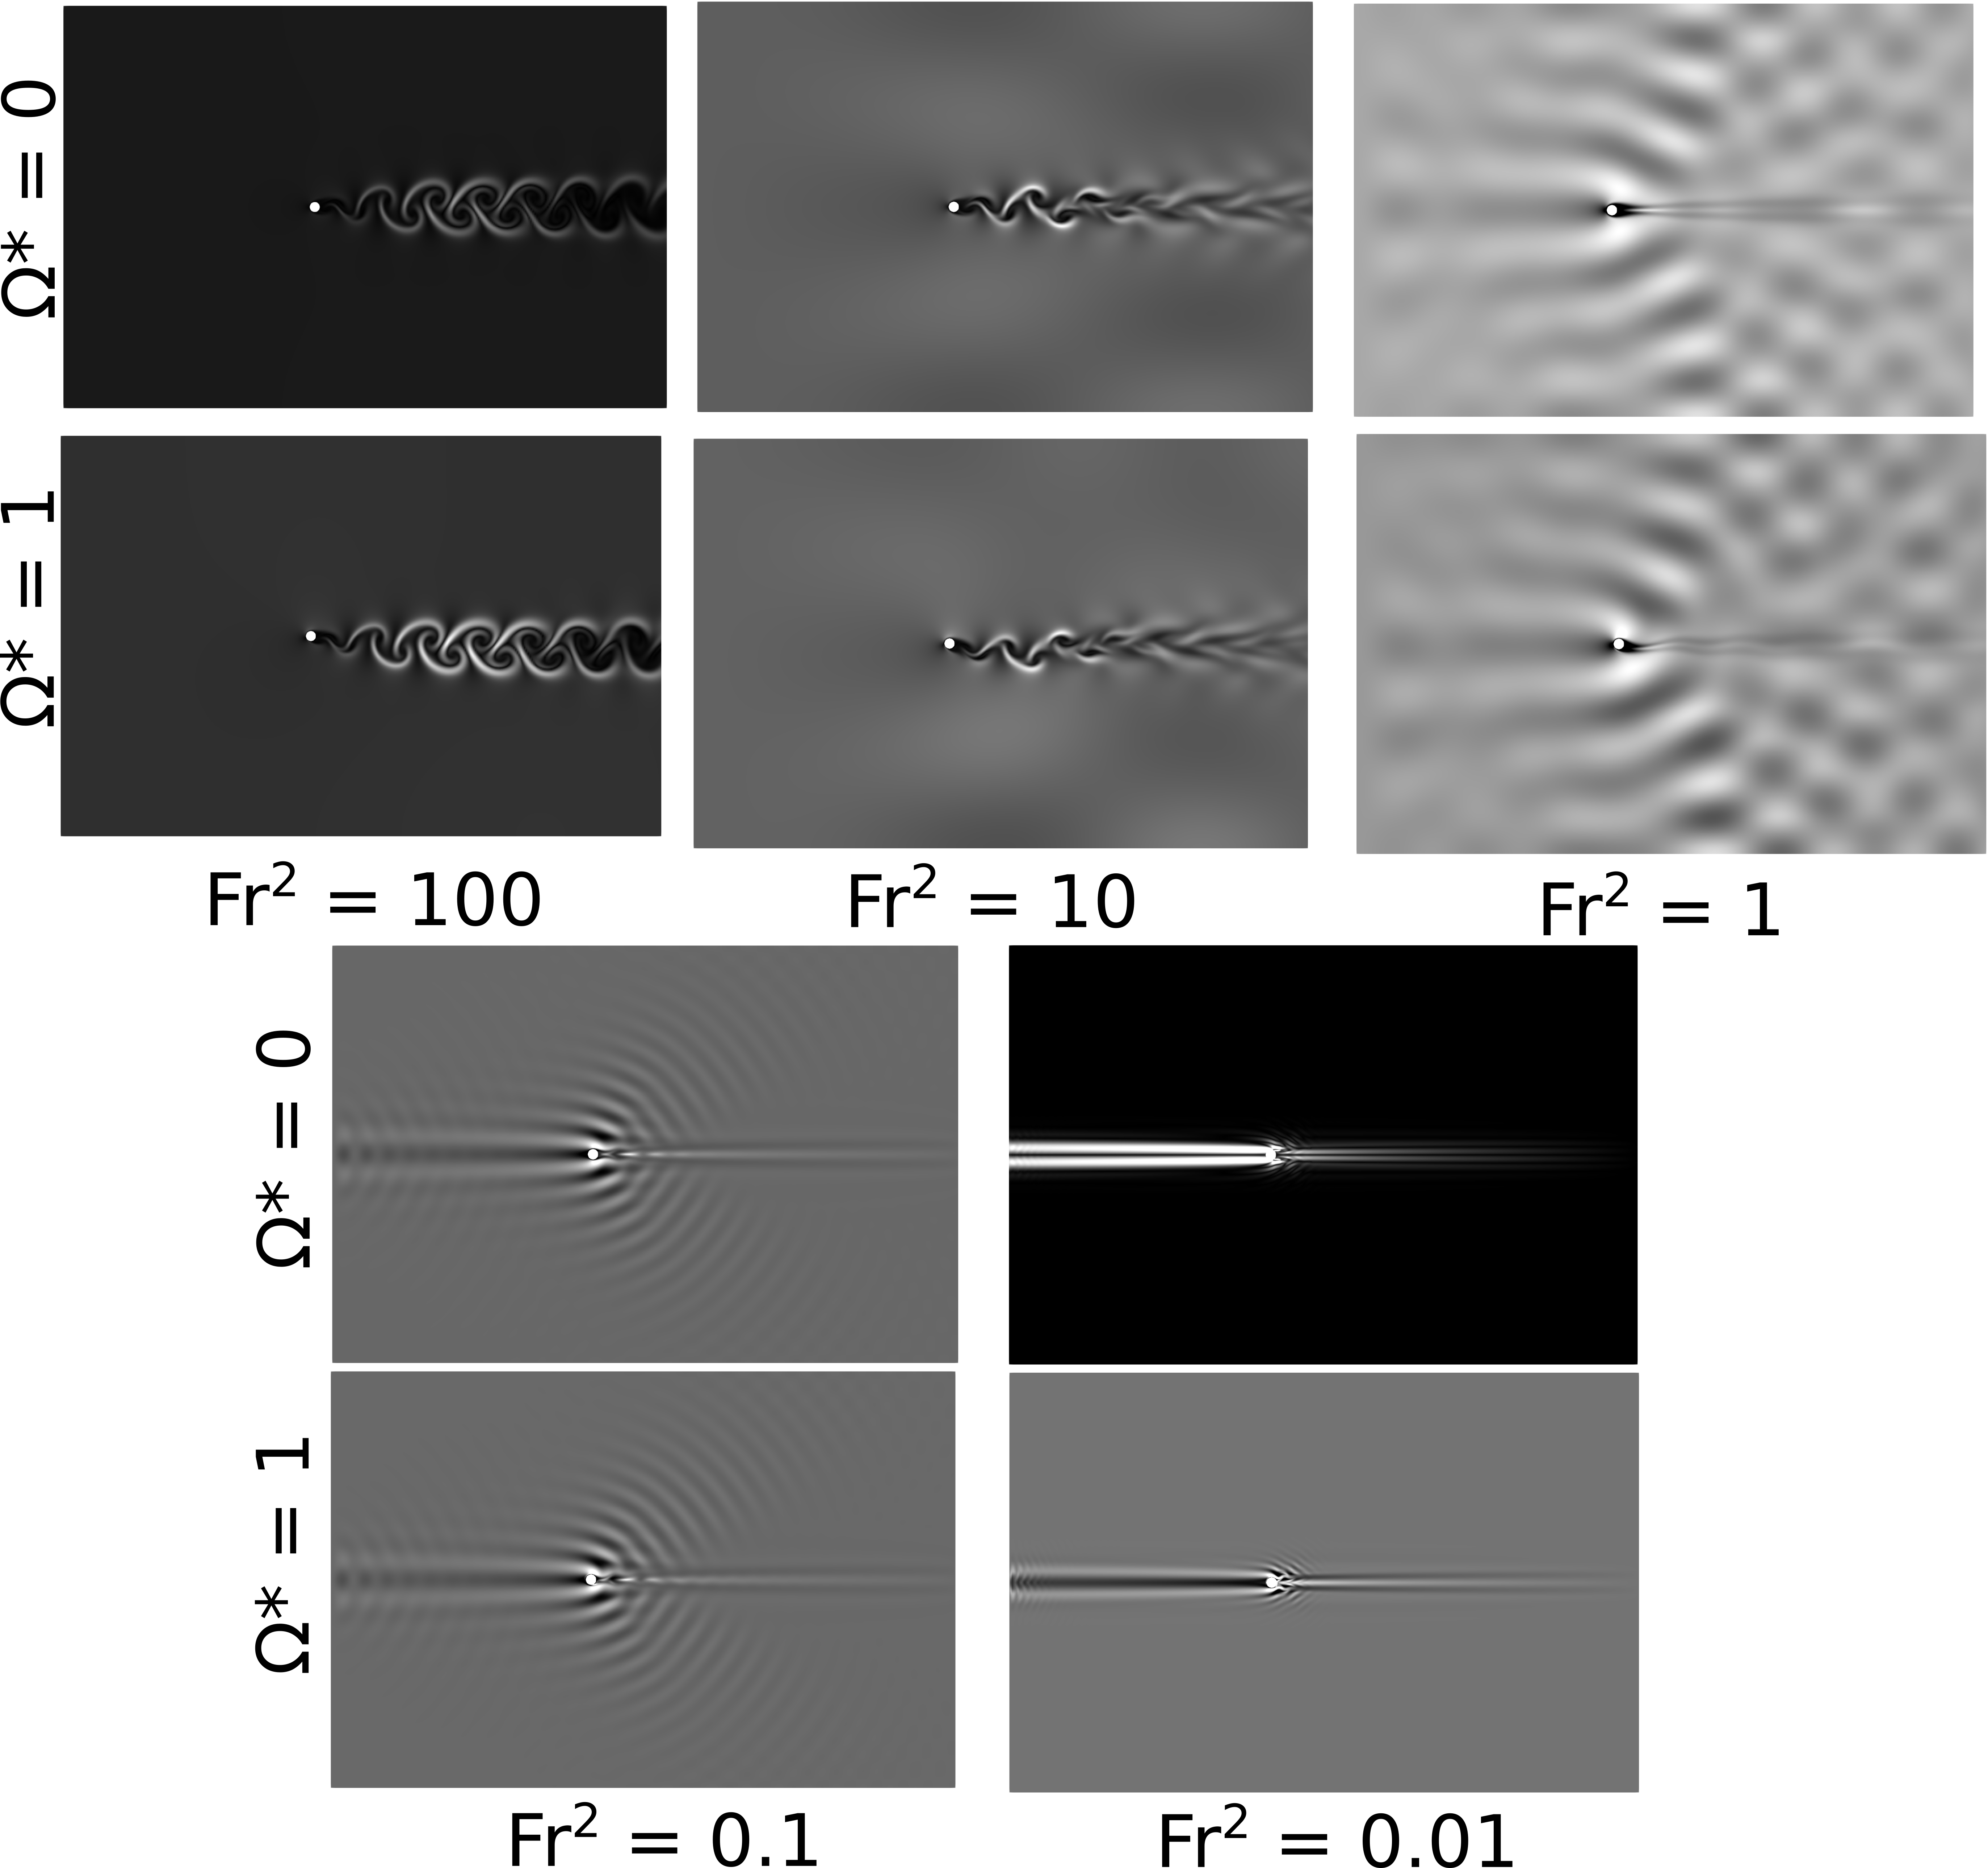
\includegraphics[width = \textwidth]{images/circle/circleschlerien.png}
    \caption{A comparison of the Schlerien fields for nonspinning and spinning circles}
    \label{fig:circleschlerien}
\end{figure}

\begin{figure}
    \centering
    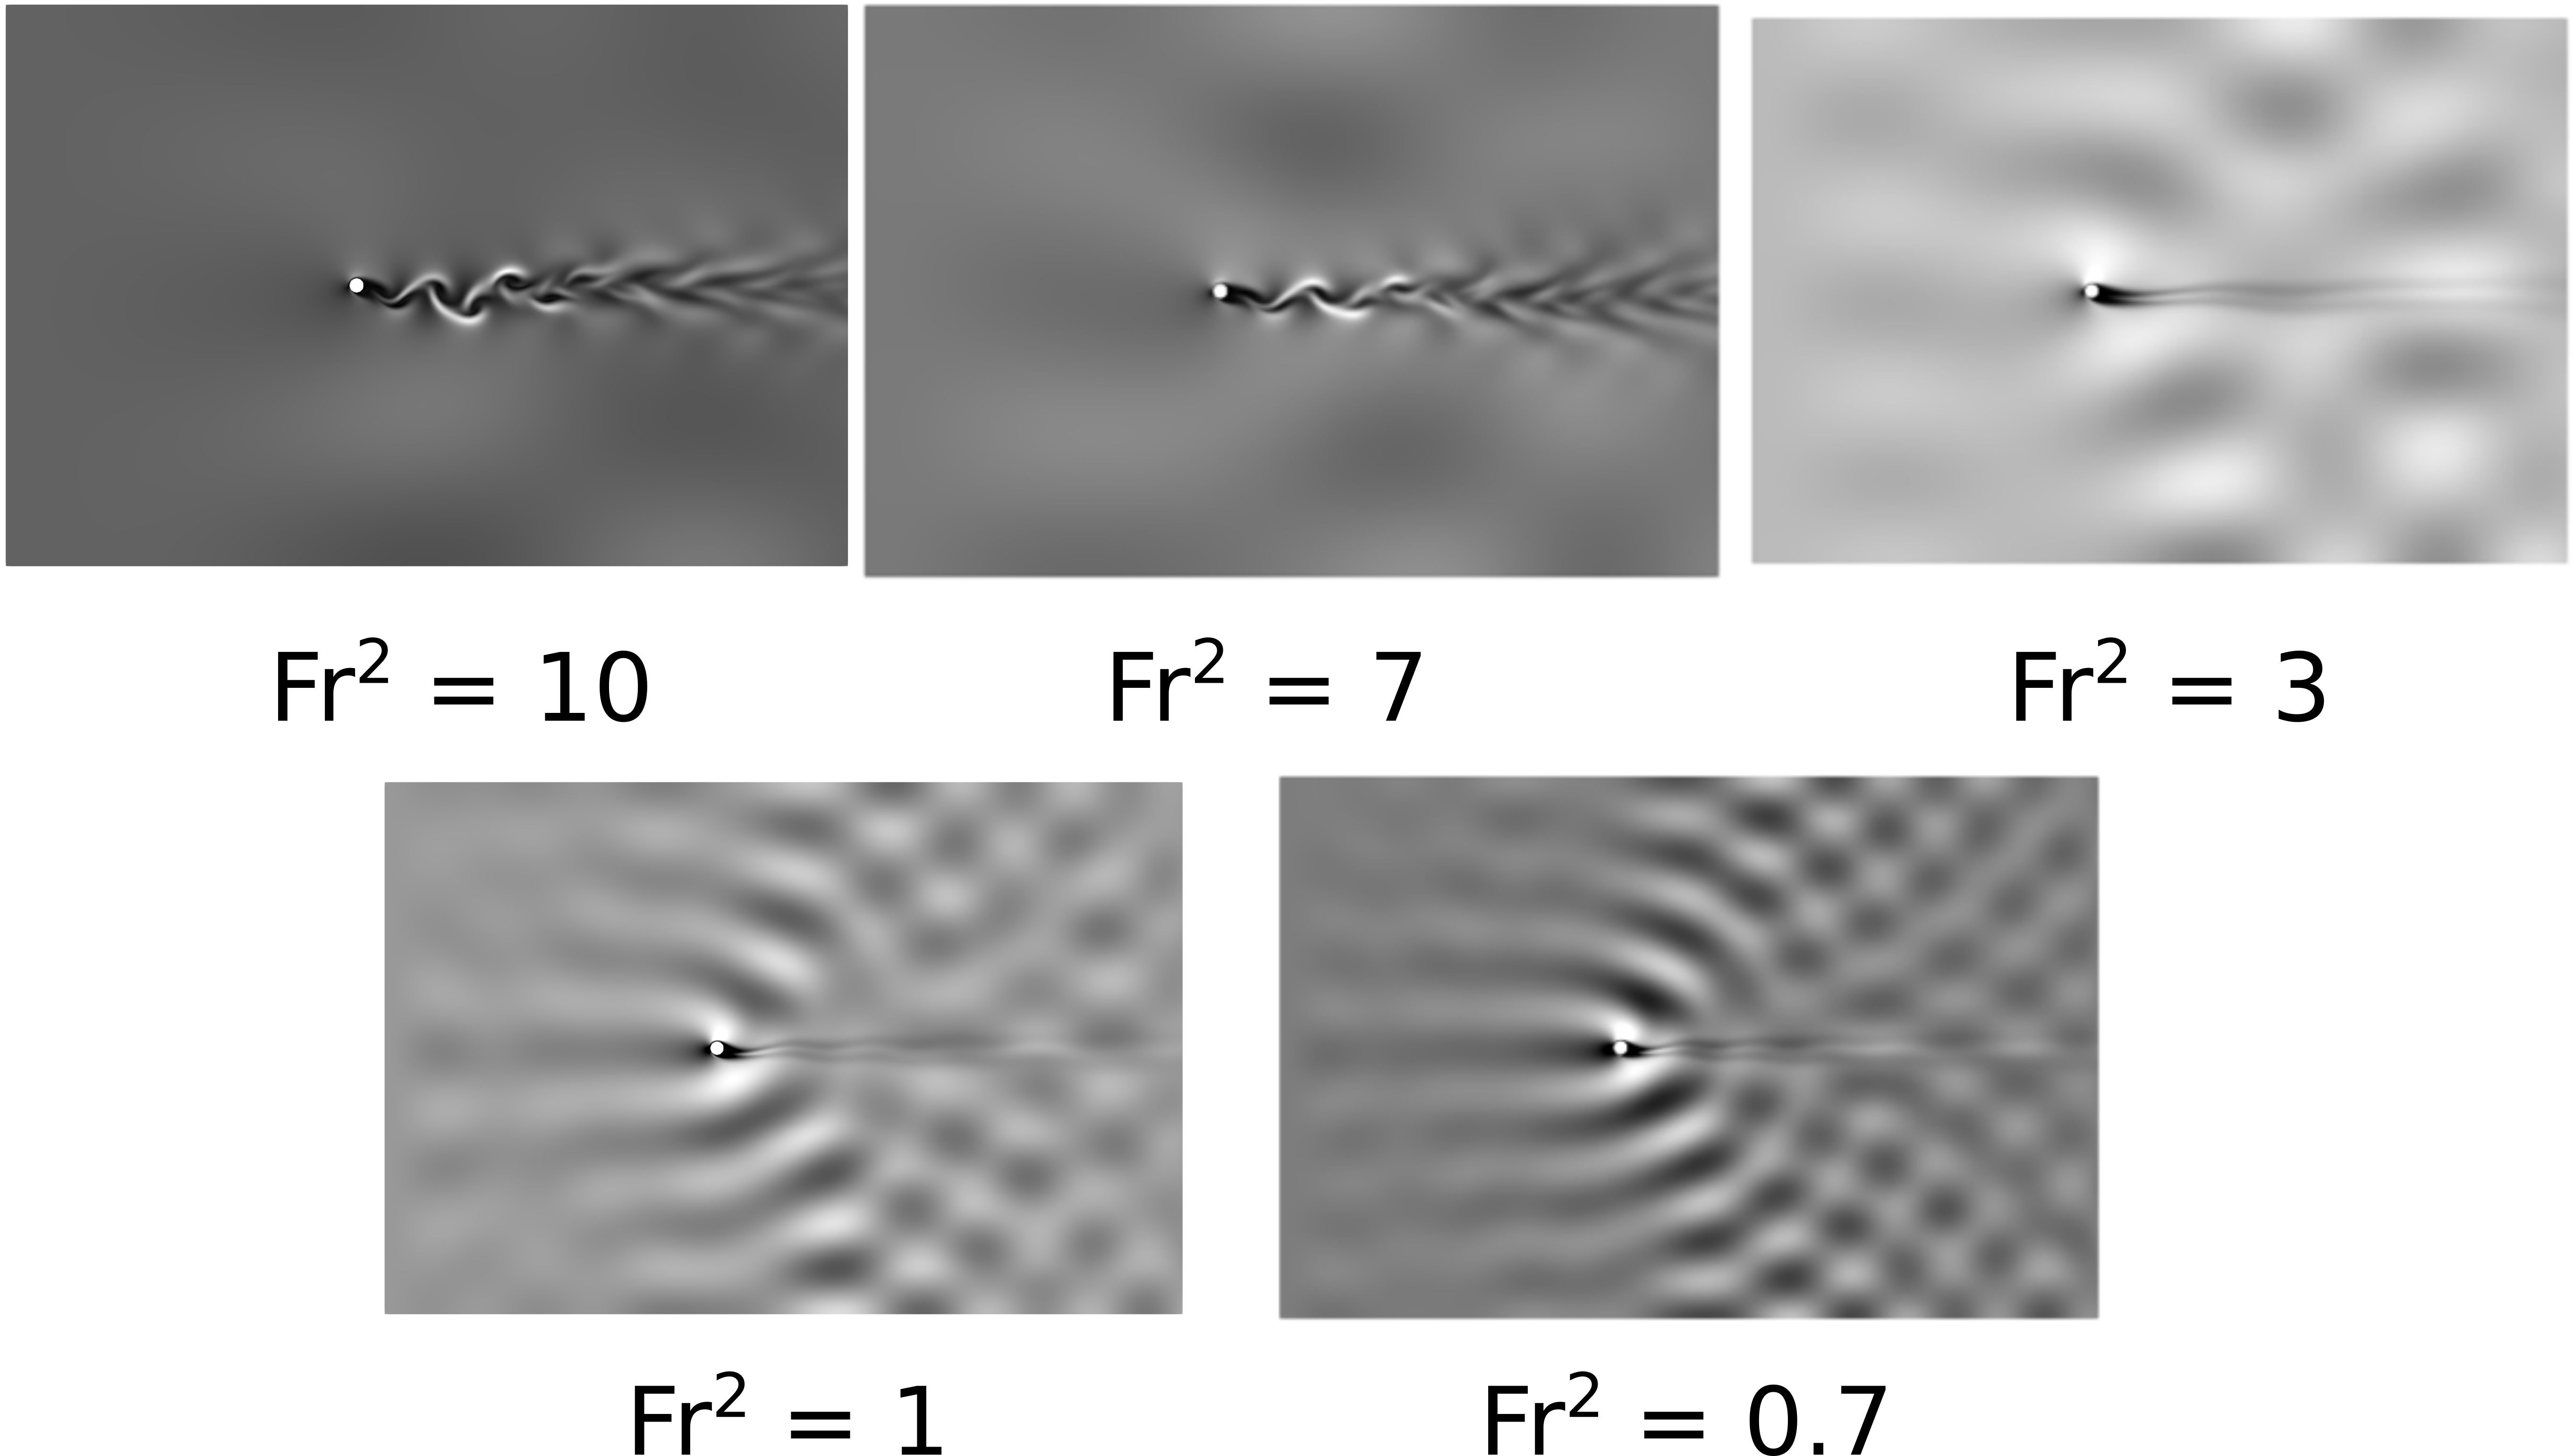
\includegraphics[width = \textwidth]{images/circle/circleschlerien2.png}
    \caption{A close look of the Schlerien plots at the transition with spin}
    \label{fig:circleschlerien2}
\end{figure}




\clearpage

\section{Spinning ellipse}
\label{section:Spinning_ellipse}
\subsection{Drag and lift}
For the spinning elliptic bodies, we look at nondimensional drag and lift force, rather than drag and lift coefficients. This is because the frontal area needed to calculate coefficients varies with time. For simplicity and consistency, we look at nondimensional forces rather than coefficients. We begin looking at the results of the spinning ellipses by observing the cycle-average plots of drag and lift to see the general trends. We briefly neglect the noise from shape-phase effects to help us identify under which parameters vortex-shedding occurs. Fig. \ref{fig:mvmean1p5} and \ref{fig:mvmean0p5} show the cycle-averaged drag and lift for the two ellipse cases. These plots show oscillation about the mean. We take the cycle-averaged values and divided by their respective averages and subtracted one. This way we can see the oscillation about the mean. We observe that even when we transform the shape of the body to a noncircular shape, we still find similar relations between flow regime and $Fr^2$. We find other similarities to the circle cases. We witness when $Fr^2 > 0.1$, there is no steady-state value. A transition occurs around $t = 100$ in the $Fr^2 = 10$ cases. The drag and lift undergo a small but distinct decrease. At $Fr^2 = 1$ there is an unsteady transition regime. 

Moving on from comparison with the circle cases, we observe vortex-shedding occurs at $Fr^2 > 1$. At $Fr^2 = 10$, it takes longer for the drag and lift values to reach a quasi-steady-state flow regime. Now that we have looked at the general trends in drag and lift, we move to looking at phase-averaged results. Figures \ref{fig:pa1p5} and \ref{fig:pa0p5} show the phase-averaged drag results for the elliptic shapes. 

An interesting insight is how at $Fr^2 = 0.1, 0.01$, in the cycle average plots, there is no oscillation , but in the phase average plots, these $Fr^2$ numbers have the largest amplitudes of oscillation. At high stratification, the vortex-shedding is suppressed, but through spinning the body overcomes large potential energy barriers to rotate. The resistance from the potential energy barrier manifests in the large amplitudes of phase-oscillation in drag and lift. Just like the ensemble average plots show, the effect of stratification on mean drag at $Fr^2 < 1$ is substantial. These effects are quantified in tables \ref{tab:fd} and \ref{tab:fl}, which show the mean, minimum, and maximum drag and lift values for the ellipses. An interesting phenomenon is how a decrease in stratification not only reduces drag, but causes it to go negative to produce thrust.  This phenomenon of thrust was previously observed in unstratified flow simulations in literature \cite{lua_rotating_2018}. Increase in stratification causes a decrease in lift. Whereas when the stratification was higher, the only substantial low-pressure zone for the ellipses was on the top, with high stratification there are low pressure zones on the top, bottom, and to the right. This explains the decrease in lift with increase in stratification for the ellipses. This is shown in figures \ref{fig:ar1p5_pressure} and \ref{fig:ar0p5_pressure}.

Another effect of increasing stratification that is found in the phase-averaging plots is the change in phase. At $Fr^2 < 1$, there is a phase-lag that increases as stratification increases. This phase-lag is larger with lift than with drag. Tables \ref{tab:max_drag} and \ref{tab:max_lift} show the angles of maximum drag and lift and help us quantify this phase-lag. The phase differences in drag from $Fr^2 = \infty$ to $Fr^2 = 0.01$ are slightly higher for lift than for drag. They are also slightly higher for the case of $AR = 1.5$ than for $AR = 0.5$. 
 
\begin{figure}
    \centerline{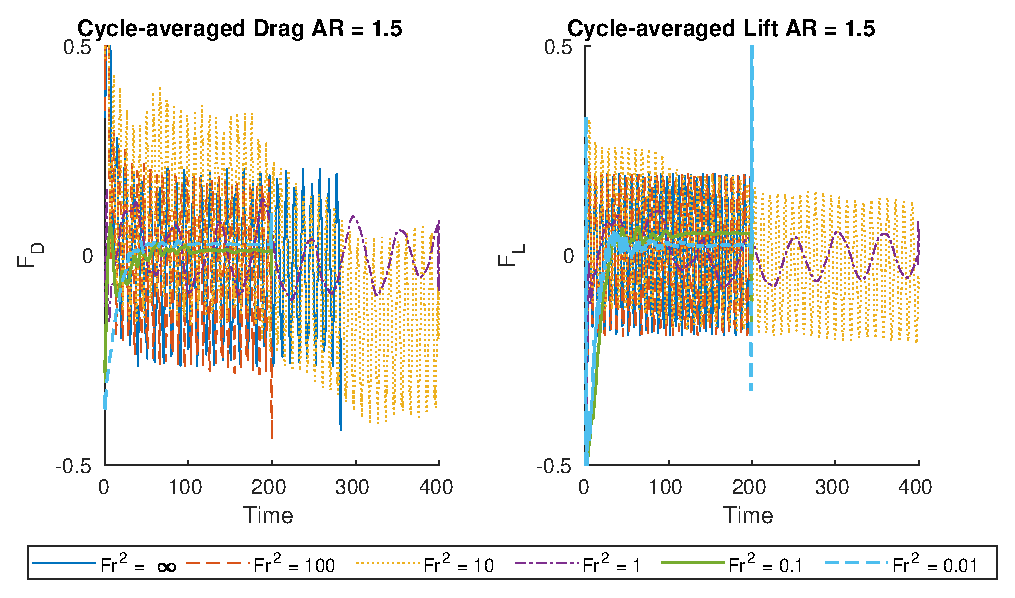
\includegraphics[width=\textwidth]{images/spinning_ellipse/mvmean1p5.eps}}
    \caption{Drag and lift over time averaged across each period for $AR = 1.5$}
    \label{fig:mvmean1p5}
\end{figure}

\begin{figure}
    \centerline{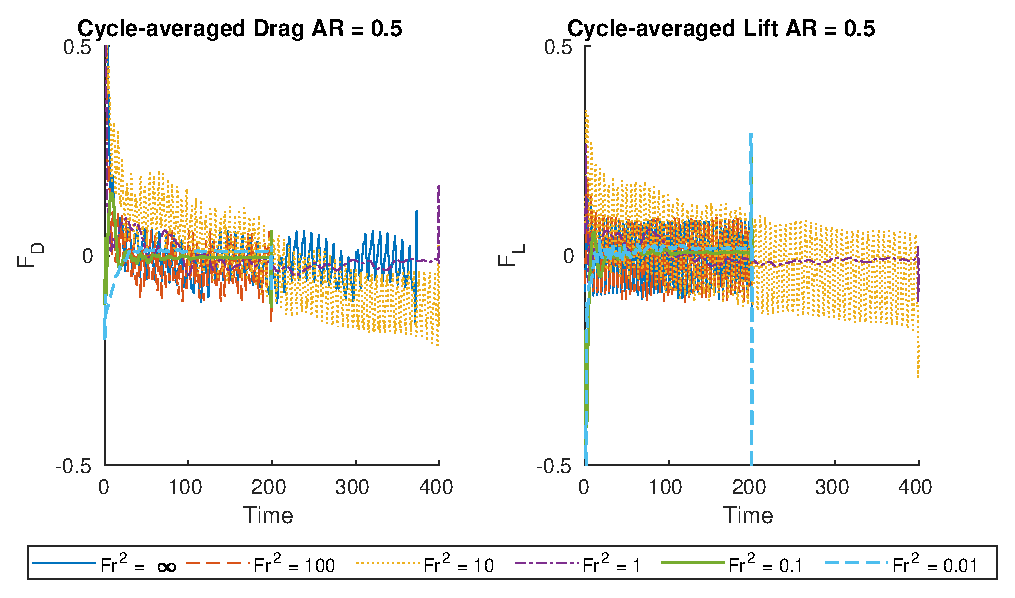
\includegraphics[width=\textwidth]{images/spinning_ellipse/mvmean0p5.eps}}
    \caption{Drag and lift over time averaged across each period for $AR = 0.5$}
    \label{fig:mvmean0p5}
\end{figure}

\begin{figure}
    \centering
    \begin{subfigure}[b]{0.49\textwidth}
        \centering
        \includegraphics[width=\textwidth]{images/spinning_ellipse/padrag1p5.eps}
        \caption{}
        \label{fig:padrag1p5}
    \end{subfigure}
    \hfill
    \begin{subfigure}[b]{0.49\textwidth}
        \centering
        \includegraphics[width=\textwidth]{images/spinning_ellipse/palift1p5.eps}
        \caption{}
        \label{fig:palift1p5}
    \end{subfigure}
    \caption{Phase averaged drag and lift for $AR = 1.5$}
    \label{fig:pa1p5}
\end{figure}
\begin{figure}
    \centering
    \begin{subfigure}[b]{0.49\textwidth}
        \centering
        \includegraphics[width=\textwidth]{images/spinning_ellipse/padrag0p5.eps}
        \caption{}
        \label{fig:padrag0p5}
    \end{subfigure}
    \hfill
    \begin{subfigure}[b]{0.49\textwidth}
        \centering
        \includegraphics[width=\textwidth]{images/spinning_ellipse/palift0p5.eps}
        \caption{}
        \label{fig:palift0p5}
    \end{subfigure}
    \caption{Phase averaged drag and lift for $AR = 0.5$}
    \label{fig:pa0p5}
\end{figure}


\begin{table}
\centering
\begin{tabular}{lcc}
                 & $AR = 1.5$                 & $AR = 0.5$                \\ \hline
 $Fr^2 = \infty$ & 0.6897 [-0.6243, 1.8059]   & 0.5221 [-0.1315, 1.1414]  \\
 $Fr^2 = 100$    & 0.6702 [-0.6033, 1.7746]   & 0.5056 [-0.1329, 1.1122]  \\
 $Fr^2 = 10$     & 0.5454 [-0.4403, 1.4905]   & 0.3792 [-0.1406, 0.8591]  \\
 $Fr^2 = 1$      & 1.2342 [0.1583, 2.3695]    & 0.5097 [0.0137, 0.9888]   \\
 $Fr^2 = 0.1$    & 4.5277 [1.8280, 7.4431]    & 1.5094 [0.3125, 2.8919]   \\
 $Fr^2 = 0.01$   & 20.1590 [12.5776, 27.9980] & 5.7467 [2.7655, 8.8887]              
\end{tabular}
\caption{$F_D$}
\label{tab:fd}
\end{table}

\begin{table}
\centering
\begin{tabular}{lcc}
                 & $AR = 1.5$                 & $AR = 0.5$                 \\ \hline
 $Fr^2 = \infty$ & 2.2945 [0.8812, 4.0093]    &  0.9607 [0.0413, 1.7659]   \\
 $Fr^2 = 100$    & 2.2582 [0.8772, 3.9185]    &  0.9423 [0.2496, 1.7367]   \\
 $Fr^2 = 10$     & 1.9083 [0.8807, 3.1827]    &  0.7696 [0.2211, 1.4244]   \\
 $Fr^2 = 1$      & 1.9595 [0.9927, 2.9782]    &  0.7648 [0.2935, 1.2389]   \\
 $Fr^2 = 0.1$    & 1.4855 [-0.1808, 2.9482]   &  0.6762 [-0.1450, 1.4325]  \\
 $Fr^2 = 0.01$   & -0.9269 [-7.5654, 6.8364]  & -0.4403 [-2.7592, 2.3845]              
\end{tabular}
\caption{$F_L$}
\label{tab:fl}
\end{table}


\begin{table}
\centering
\begin{tabular}{lcc}
                 & $AR = 1.5$          & $AR = 0.5$         \\ \hline
 $Fr^2 = \infty$ & 139.7701, 319.7700  & 57.3299, 237.6899  \\
 $Fr^2 = 100$    & 140.3099, 320.8501  & 57.3299, 236.9701  \\
 $Fr^2 = 10$     & 141.2094, 321.7503  & 56.0703, 236.2502  \\
 $Fr^2 = 1$      & 153.8103, 334.1700  & 63.0899, 242.7300  \\
 $Fr^2 = 0.1$    & 159.5702, 339.5697  & 71.1906, 251.3700  \\
 $Fr^2 = 0.01$   & 176.1301, 356.1304  & 85.2299, 265.2300             
\end{tabular}
\caption{Max drag angles}
\label{tab:max_drag}
\end{table}

\begin{table}
\centering
\begin{tabular}{lcc}
                 & $AR = 1.5$          & $AR = 0.5$         \\ \hline
 $Fr^2 = \infty$ & 92.6103, 271.3496   & 8.0099, 189.6304   \\
 $Fr^2 = 100$    & 92.4299, 273.6899   & 8.0099, 187.6501   \\
 $Fr^2 = 10$     & 93.3300, 274.7704   & 6.5699, 187.6500   \\
 $Fr^2 = 1$      & 99.9902, 280.7099   & 10.3505, 190.5300  \\
 $Fr^2 = 0.1$    & 107.3702, 287.1896  & 35.0101, 214.8302  \\
 $Fr^2 = 0.01$   & 134.0096, 314.0104  & 47.6098, 227.6099             
\end{tabular}
\caption{Max lift angles}
\label{tab:max_lift}
\end{table}
\begin{figure}
    \centering
    \begin{subfigure}[b]{0.25\textwidth}
        \centering
        \includegraphics[width=\textwidth]{images/spinning_ellipse/par1p5fsinf.png}
        \caption{$Fr^2 = \infty$}
        \label{fig:par1p5fsinf}
    \end{subfigure}
    \hfill
    \begin{subfigure}[b]{0.25\textwidth}
        \centering
        \includegraphics[width=\textwidth]{images/spinning_ellipse/par1p5fs100.png}
        \caption{$Fr^2 = 100$}
        \label{fig:par1p5fs100}
    \end{subfigure}
    \hfill
    \begin{subfigure}[b]{0.25\textwidth}
        \centering
        \includegraphics[width=\textwidth]{images/spinning_ellipse/par1p5fs10.png}
        \caption{$Fr^2 = 10$}
        \label{fig:par1p5fs10}
    \end{subfigure}
    
    \begin{subfigure}[b]{0.25\textwidth}
        \centering
        \includegraphics[width=\textwidth]{images/spinning_ellipse/par1p5fs1.png}
        \caption{$Fr^2 = 1$}
        \label{fig:par1p5fs1}
    \end{subfigure}
    \hfill
    \begin{subfigure}[b]{0.25\textwidth}
        \centering
        \includegraphics[width=\textwidth]{images/spinning_ellipse/par1p5fs0p1.png}
        \caption{$Fr^2 = 0.1$}
        \label{fig:par1p5fs0p1}
    \end{subfigure}
    \hfill
    \begin{subfigure}[b]{0.25\textwidth}
        \centering
        \includegraphics[width=\textwidth]{images/spinning_ellipse/par1p5fs0p01.png}
        \caption{$Fr^2 = 0.01$}
        \label{fig:par1p5fs0p01}
    \end{subfigure}
    
    \begin{subfigure}[b]{0.25\textwidth}
        \centering
        \includegraphics[width=\textwidth]{images/spinning_ellipse/p_scale.png}
        \caption*{}
    \end{subfigure}
    
    \caption{A comparison of the pressure fields for spinning ellipse where $AR = 1.5$}
    \label{fig:ar1p5_pressure}
\end{figure}

\begin{figure}
    \centering
    \begin{subfigure}[b]{0.25\textwidth}
        \centering
        \includegraphics[width=\textwidth]{images/spinning_ellipse/par0p5fsinf.png}
        \caption{$Fr^2 = \infty$}
        \label{fig:par0p5fsinf}
    \end{subfigure}
    \hfill
    \begin{subfigure}[b]{0.25\textwidth}
        \centering
        \includegraphics[width=\textwidth]{images/spinning_ellipse/par0p5fs100.png}
        \caption{$Fr^2 = 100$}
        \label{fig:par0p5fs100}
    \end{subfigure}
    \hfill
    \begin{subfigure}[b]{0.25\textwidth}
        \centering
        \includegraphics[width=\textwidth]{images/spinning_ellipse/par0p5fs10.png}
        \caption{$Fr^2 = 10$}
        \label{fig:par0p5fs10}
    \end{subfigure}
    
    \begin{subfigure}[b]{0.25\textwidth}
        \centering
        \includegraphics[width=\textwidth]{images/spinning_ellipse/par0p5fs1.png}
        \caption{$Fr^2 = 1$}
        \label{fig:par0p5fs1}
    \end{subfigure}
    \hfill
    \begin{subfigure}[b]{0.25\textwidth}
        \centering
        \includegraphics[width=\textwidth]{images/spinning_ellipse/par0p5fs0p1.png}
        \caption{$Fr^2 = 0.1$}
        \label{fig:par0p5fs0p1}
    \end{subfigure}
    \hfill
    \begin{subfigure}[b]{0.25\textwidth}
        \centering
        \includegraphics[width=\textwidth]{images/spinning_ellipse/par0p5fs0p01.png}
        \caption{$Fr^2 = 0.01$}
        \label{fig:par0p5fs0p01}
    \end{subfigure}
    
    \begin{subfigure}[b]{0.25\textwidth}
        \centering
        \includegraphics[width=\textwidth]{images/spinning_ellipse/p_scale.png}
        \caption*{}
    \end{subfigure}
    
    \caption{A comparison of the pressure fields for spinning ellipse where $AR = 0.5$}
    \label{fig:ar0p5_pressure}
\end{figure}
\clearpage
\subsubsection{Flow structures}
Figures \ref{fig:ar1p5 y-vel} and \ref{fig:ar0p5 y-vel} show similar flow patterns observed in the circular cases. The gravity waves propagate most strongly at around $Fr^2 = 1$. The plots also show a flow regime transition around $Fr^2 = 1$. We observe that with both aspect ratios, just like in the results from literature \cite{ortiz-tarin_stratified_2019}, there are circular patterns in the y-velocity around the body. Just like in the circular cases, we observe a transition in the flow type around $Fr^2 = 1$. At $Fr^2$, we see the gravity waves breaking up the paths of vortices.  Although the flow structures look the same for both aspect ratios, we observe that the magnitudes in the case of $AR = 1.5$ are larger. This is because even though $\Rey$ is the same based on our methodology, the \textit{effective} $\Rey$ increases with aspect ratio due to the larger of momentum effects from the larger body. An interesting insight is how little effect the aspect ratio has on the flow structures. Higher aspect ratio bodies show slightly larger magnitudes in the y-velocity plots, but the structures of the features look the same. We observed periodic semi-circular patterns y-velocity fields at $Fr^2 = 1, 0.1$ like in literature \cite{ortiz-tarin_stratified_2019}. Figures \ref{fig:schlerienar1p5} and \ref{fig:schlerienar0p5} give us schlerien plots of the spinning ellipses. ANTON NEEDS TO LOOK MORE AT TRANSITIONS
\begin{figure}
    \centering
    \begin{subfigure}[b]{0.32\textwidth}
        \centering
        \includegraphics[width=\textwidth]{images/spinning_ellipse/ar1p5fsinf.png}
        \caption{$Fr^2 = \infty$}
        \label{fig:ar1p5fsinf}
    \end{subfigure}
    \hfill
    \begin{subfigure}[b]{0.32\textwidth}
        \centering
        \includegraphics[width=\textwidth]{images/spinning_ellipse/ar1p5fr10.png}
        \caption{$Fr^2 = 100$}
        \label{fig:ar1p5fr10}
    \end{subfigure}
    \hfill
    \begin{subfigure}[b]{0.32\textwidth}
        \centering
        \includegraphics[width=\textwidth]{images/spinning_ellipse/ar1p5fr3.png}
        \caption{$Fr^2 = 10$}
        \label{fig:ar1p5fr3}
    \end{subfigure}
    
    \begin{subfigure}[b]{0.32\textwidth}
        \centering
        \includegraphics[width=\textwidth]{images/spinning_ellipse/ar1p5fr1.png}
        \caption{$Fr^2 = 1$}
        \label{fig:ar1p5fr1}
    \end{subfigure}
    \hfill
    \begin{subfigure}[b]{0.32\textwidth}
        \centering
        \includegraphics[width=\textwidth]{images/spinning_ellipse/ar1p5fr0p3.png}
        \caption{$Fr^2 = 0.1$}
        \label{fig:ar1p5fr0p3}
    \end{subfigure}
    \hfill
    \begin{subfigure}[b]{0.32\textwidth}
        \centering
        \includegraphics[width=\textwidth]{images/spinning_ellipse/ar1p5fr0p1.png}
        \caption{$Fr^2 = 0.01$}
        \label{fig:ar1p5fr0p1}
    \end{subfigure}
    
    \begin{subfigure}[b]{0.32\textwidth}
        \centering
        \includegraphics[width=\textwidth]{images/spinning_ellipse/scale1.png}
        \caption*{}
    \end{subfigure}
    
    \caption{A comparison of the y-velocity fields for spinning ellipse where $AR = 1.5$}
    \label{fig:ar1p5 y-vel}
\end{figure}

\begin{figure}
    \centering
    \begin{subfigure}[b]{0.32\textwidth}
        \centering
        \includegraphics[width=\textwidth]{images/spinning_ellipse/ar0p5fsinf.png}
        \caption{$Fr^2 = \infty$}
        \label{fig:ar0p5fsinf}
    \end{subfigure}
    \hfill
    \begin{subfigure}[b]{0.32\textwidth}
        \centering
        \includegraphics[width=\textwidth]{images/spinning_ellipse/ar0p5fr10.png}
        \caption{$Fr^2 = 100$}
        \label{fig:ar0p5fr10}
    \end{subfigure}
    \hfill
    \begin{subfigure}[b]{0.32\textwidth}
        \centering
        \includegraphics[width=\textwidth]{images/spinning_ellipse/ar0p5fr3.png}
        \caption{$Fr^2 = 10$}
        \label{fig:ar0p5fr3}
    \end{subfigure}
    
    \begin{subfigure}[b]{0.32\textwidth}
        \centering
        \includegraphics[width=\textwidth]{images/spinning_ellipse/ar0p5fr1.png}
        \caption{$Fr^2 = 1$}
        \label{fig:ar0p5fr1}
    \end{subfigure}
    \hfill
    \begin{subfigure}[b]{0.32\textwidth}
        \centering
        \includegraphics[width=\textwidth]{images/spinning_ellipse/ar0p5fr0p3.png}
        \caption{$Fr^2 = 0.1$}
        \label{fig:ar0p5fr0p3}
    \end{subfigure}
    \hfill
    \begin{subfigure}[b]{0.32\textwidth}
        \centering
        \includegraphics[width=\textwidth]{images/spinning_ellipse/ar0p5fr0p1.png}
        \caption{$Fr^2 = 0.01$}
        \label{fig:ar0p5fr0p1}
    \end{subfigure}
    
    \begin{subfigure}[b]{0.32\textwidth}
        \centering
        \includegraphics[width=\textwidth]{images/spinning_ellipse/scale1.png}
        \caption*{}
    \end{subfigure}
    
    \caption{A comparison of the y-velocity fields for spinning ellipse where $AR = 0.5$}
    \label{fig:ar0p5 y-vel}
\end{figure}
\begin{figure}
    \centering
    \includegraphics[width = \textwidth]{images/spinning_ellipse/schlerienar1p5.png}
    \caption{A comparison of the Schlerien fields for spinning ellipse where $AR = 1.5$}
    \label{fig:schlerienar1p5}
\end{figure}

\begin{figure}
    \centering
    \includegraphics[width=\textwidth]{images/spinning_ellipse/schlerienar0p5.png}
    \caption{A comparison of the Schlerien fields for spinning ellipse where $AR = 0.5$}
    \label{fig:schlerienar0p5}
\end{figure}


    
    % Endmatter
    % For BibTeX references: specify a .bib file and a style.
    % The style used here is for IEEE transactions formatting:
    \references{IEEEabrv,sample,lib}{IEEEtran}
    % The style used here is for AIAA formatting:
%    \references{IEEEabrv,sample}{aiaa}
    
    %
%  Example Appendix pages.
%  Modified to use new usu-thesis-mk2 appendix facilities.
%
%  Time-stamp: "[appendix.tex] last modified by Scott Budge (scott) on 2011-08-08 (Monday, 8 August 2011) at 15:46:06 on goga"
%
%  Info: $Id$   USU
%  Revision: $Rev$
% $LastChangedDate$
% $LastChangedBy$
%
%
% For a single appendix, use \makeappendix, and place the 
% body of the appendix after it

%\makeappendix

% < single appendix body here >

% For multiple appendices, use \makeappendices, and create each appendix
% using \appendix{}
% For sub-appendices use \appendixsection{} and \appendixsubsection{}

\makeappendices
\appendix{List of Edge Vectors}
\label{chap:appendix}


\appendixsection{Definition of an Edge Vector}
\label{sec:edge-def}

Before we list the table of edge vectors, we need to describe what an
edge vector is.  In this section we will describe in detail the theory
that results in the edge vectors.  The first set of edge vectors is
given in Table~\ref{table1}.

\begin{table}[!t]
% increase table row spacing, adjust to taste
  \renewcommand{\arraystretch}{1.3}

  \caption{List of edge vectors for a codebook with b=8 and d=3, for a
    $4 \times 4$ vector size.}
  \label{table1}

  \centering
  \begin{tabular}{|c|c|} \hline
    Level & Edge Vectors \\ \hline

    & (5) \\ 
    L1 & (6) \\
    & (7) \\ \hline

    & (3,1)\\
    & (3,2)\\
    & (3,5)\\
    & (4,0)\\
    L2 & (4,2)\\
    & (4,3)\\
    & (4,4)\\
    & (4,5)\\
    & (4,6) \\ \hline

    & (3,4,1)\\
    & (3,4,2)\\
    & (3,7,0)\\
    & (3,7,2)\\
    & (3,7,4)\\
    L3 & (4,1,0)\\
    & (4,1,1)\\
    & (4,1,2)\\
    & (4,1,3)\\
    & (4,1,4)\\
    & (4,1,5)\\
    & (4,1,6) \\ \hline

  \end{tabular}

\end{table}


\appendixsection{Next Codebook Size Description}
\label{sec:next-size}

In this section we do the next size codebook.  This is different from
the previous case in that the codebook size is different.  The next
set of edge vectors is given in Table \ref{table2}.

\appendixsection{Final Set of  Codebook Size Descriptions}
\label{sec:final-size}

The following three tables contain the data for codebook sizes that
are different than the previous sizes.  We note that the differences
in the tables are due to the differences in the sizes of the codebook
edge vectors.  Note the values given in Table \ref{table3} --
Table \ref{table5}.


\begin{table}[!t]
  \renewcommand{\arraystretch}{1.3}
  \centering

  \caption{List of edge vectors for a codebook with b=4 and d=3, for a
    $4 \times 4$ vector size.}
  \label{table2}

  \begin{tabular}{|c|c|} \hline
    Level & Edge Vectors \\ \hline

    & (1)\\
    L1 & (2)\\
    & (3) \\ \hline

    L2 & (0,3) \\ \hline

    & (0,2,0)\\
    L3 & (0,2,2)\\
    & (0,2,3) \\ \hline

  \end{tabular}

\end{table}

\begin{table}[!t]
  \renewcommand{\arraystretch}{1.3}
  \centering

  \caption{List of edge vectors for a codebook with b=16 and d=3, for
    a $4 \times 4$ vector size.}
  \label{table3}

  \begin{tabular}{|c|c|} \hline
    Level & Edge Vectors \\ \hline

    & (11)\\
    & (12)\\
    L1 & (13)\\
    & (14)\\
    & (15) \\ \hline

    & (7,0)\\
    & (7,1)\\
    & (7,2)\\
    & (7,6)\\
    L2 & (8,4)\\
    & (8,5)\\
    & (8,6)\\
    & (9,6)\\
    & (9,14)\\
    & (10,1) \\ \hline

    & (4,6,14)\\
    & (5,6,6)\\
    & (6,14,0)\\
    & (6,14,3)\\
    L3 & (6,14,4)\\
    & (6,14,5)\\
    & (7,7,0)\\
    & (7,14,7)\\
    & (9,5,3)\\
    & (9,5,10)\\
    & (9,5,11) \\ \hline

  \end{tabular}

\end{table}

\begin{table}[!t]
  \renewcommand{\arraystretch}{1.3}
  \centering

  \caption{ List of edge vectors for a codebook with b=16 and d=3, for
    a $2 \times 2$ vector size.}
  \label{table4}

  \begin{tabular}{|c|c|} \hline
    Level & Edge Vectors \\ \hline

    & (9)\\
    & (10)\\
    L1 & (11)\\
    & (12)\\
    & (13) \\ \hline

    L2 & (6,0)\\
    & (6,3) \\ \hline

    & (2,2,8)\\
    & (6,5,1)\\
    & (6,5,4)\\
    & (6,5,6)\\
    & (6,5,7)\\
    & (6,5,8)\\
    L3 & (6,5,15)\\
    & (7,0,14)\\
    & (8,0,1)\\
    & (8,15,3)\\
    & (8,15,4)\\
    & (8,15,10) \\ \hline

  \end{tabular}

\end{table}

\begin{table}[!t]
  \renewcommand{\arraystretch}{1.3}
  \centering

  \caption{ List of edge vectors for a codebook with b=16 and d=3, for
    a $6 \times 6$ vector size.}
  \label{table5}

  \begin{tabular}{|c|c|} \hline
    Level & Edge Vectors \\ \hline

    & (6)\\
    & (7)\\
    & (8)\\
    & (9)\\
    L1 & (10)\\
    & (11)\\
    & (12)\\
    & (13)\\
    & (14)\\
    & (15) \\ \hline

    & (2,8)\\
    & (2,13)\\
    & (4,1)\\
    & (4,6)\\
    L2 & (4,7)\\
    & (4,8)\\
    & (4,10)\\
    & (4,11)\\
    & (4,13)\\
    & (4,15) \\ \hline

    & (1,7,0)\\
    & (1,7,1)\\
    & (1,7,2)\\
    L3 & (1,7,3)\\
    & (1,7,4)\\
    & (1,7,6)\\
    & (1,7,9)\\
    & (1,7,12) \\ \hline

  \end{tabular}

\end{table}

\appendix{Another Example Appendix}


\appendixsection{Background}
\label{sec:back}


Some random appended text for this section of the appendix....


\appendixsection{Meat of the Appendix}
\label{sec:meat}

Here we have the data that is so important to be included in this
appendix.

    %
% This is an example of a vita page.  
% Format is not tightly specified. This example comes from Lili Ma.
%
%  Time-stamp: "[vita.tex] last modified by Scott Budge (scott) on 2012-07-16 (Monday, 16 July 2012) at 11:18:06 on goga"
%
%  Info: $Id$   USU
%  Revision: $Rev$
% $LastChangedDate$
% $LastChangedBy$
%

\begin{vita}

\begin{center}
{\Large \bf John Q. Engineer}\\
\end{center}

\section*{Published Journal Articles}
    \begin{itemize}
    \item Rational Radial Distortion Models of Camera Lenses with Analytical Solution for Distortion Correction, Lili
    Ma, YangQuan Chen, and Kevin L. Moore, {\it International Journal of Information Acquisition}, {\it Accepted}.

    \item A Small Mobile Robot for Security and Inspection Operations, N.S. Flann, K. L. Moore, and Lili Ma, {\it Control Engineering Practice}, vol. 10, pp. 1265-1270,
    2002.
    \end{itemize}

\section*{Published Conference Papers}
    \begin{itemize}
    \item Range Identification for Perspective Dynamic Systems Using
      Linear Approximation, Lili Ma, YangQuan Chen, and Kevin
      L. Moore, in {\it Proc. IEEE Int. Conf. on Robotics and
        Automation (ICRA)},
    2004.
  \item Range Identification for Perspective Dynamic System with
    Single Homogeneous Observation, Lili Ma, YangQuan Chen, and Kevin
    L. Moore, in {\it Proc. IEEE Int. Conf. on Robotics and Automation (ICRA)},
    2004.
  \item Blind Detection and Compensation of Camera Lens Geometrical
    Distortions, Lili Ma and YangQuan Chen, {\it SIAM Imaging
      Science}, 2004.
  \item Flexible Camera Calibration Using a New Analytical Radial
    Undistortion Formula with Application to Mobile Robot
    Localization, Lili Ma, YangQuan Chen, and Kevin L. Moore, in {\it
      Proc. Int. Symposium on Intelligent Control (ISIC)}, 2003.
  \item Sonar and Laser Based HIMM Map Building for Collision
    Avoidance for Mobile Robots, Lili Ma and Kevin L. Moore, in {\it
      Proc. International Symposium on Intelligent Control (ISIC)},
    2003.
  \item Wireless Visual Servoing for ODIS - An Under Car Inspection
    Mobile Robot, Lili Ma, Matthew Berkemeier, YangQuan Chen, Morgan
    Davidson, Vikas Bahl, and Kevin L. Moore, in {\it Proc. IFAC World
      Congress}, Spain, July, 2002.
  \item Visual Servoing of an Omni-Directional Mobile Robot for
    Alignment with Parking Lot Lines, Matthew Berkemeier, Morgan
    Davidson, Vikas Bahl, YangQuan Chen, and Lili Ma, in {\it Proc.
      IEEE Int.  Conf. on Robotics and Automation (ICRA)}, May 2002.
  \item Some Sensing and Perception Techniques for an Omnidirectional
    Ground Vehicle with a Laser Scanner, Zhen Song, YangQuan Chen,
    Lili Ma, and You Chung Chung, in {\it Proc. IEEE Int. Symposium on
      Intelligent Control (ISIC)}, October 2002.
  \item A Small Mobile Robot For Security and Inspection Operations,
    Flann NS, Moore KL, and Ma L, in {\it Proc. IFAC Conference on Telematics
      Applications in Automation and Robotics}, July 2001.
    \end{itemize}

\end{vita}
 %This is optional for the Thesis proposal or Dissertation proposal but is REQUIRED for the Thesis or Dissertation!!!
    %}}}
\end{document}
